% !TeX document-id = {7f59beb7-c93a-43bd-a036-7847a50120d2}
% !TeX spellcheck = en_US
% !TeX program = make
% Dieses Dokument muss mit PDFLatex gesetzt werden
% Vorteil: Grafiken koennen als jpg, png, ... verwendet werden
%          und die Links im Dokument sind auch gleich richtig
%
%Ermöglicht \\ bei der Titelseite (z.B. bei supervisor)
%Siehe https://github.com/latextemplates/uni-stuttgart-cs-cover/issues/4
\RequirePackage{kvoptions-patch}

%English:
\let\ifdeutsch\iffalse
\let\ifenglisch\iftrue

%German:
%\let\ifdeutsch\iftrue
%\let\ifenglisch\iffalse

%
\ifenglisch
	\PassOptionsToClass{numbers=noenddot}{scrbook}
\else
	%()Aus scrguide.pdf - der Dokumentation von KOMA-Script)
	%Nach DUDEN steht in Gliederungen, in denen ausschließlich arabische Ziffern für die Nummerierung
	%verwendet werden, am Ende der Gliederungsnummern kein abschließender Punkt
	%(siehe [DUD96, R3]). Wird hingegen innerhalb der Gliederung auch mit römischen Zahlen
	%oder Groß- oder Kleinbuchstaben gearbeitet, so steht am Ende aller Gliederungsnummern ein
	%abschließender Punkt (siehe [DUD96, R4])
	\PassOptionsToClass{numbers=autoendperiod}{scrbook}
\fi

%Warns about outdated packages and missing caption delcarations
%See https://www.ctan.org/pkg/nag
\RequirePackage[l2tabu, orthodox]{nag}

%Neue deutsche Trennmuster
%Siehe http://www.ctan.org/pkg/dehyph-exptl und http://projekte.dante.de/Trennmuster/WebHome
%Nur für pdflatex, nicht für lualatex
\RequirePackage{ifluatex}
\ifluatex
%do not load anything
\else
	\ifdeutsch
		\RequirePackage[ngerman=ngerman-x-latest]{hyphsubst}
	\fi
\fi

\documentclass[
               fontsize=12pt, %Default: 11pt, bei Linux Libertine zu klein zum Lesen
% BEGINN: Optionen für typearea
               paper=a4,
               twoside,  % fuer die Betrachtung am Schirm ungeschickt
               BCOR=3mm, % Bindekorrektur
               DIV=13,   % je höher der DIV-Wert, desto mehr geht auf eine Seite. Gute werde sind zwischen DIV=12 und DIV=15
               headinclude=true,
               footinclude=false,
% ENDE: Optionen für typearea
%               titlepage,
               bibliography=totoc,
%               idxtotoc,   %Index ins Inhaltsverzeichnis
%                liststotoc, %List of X ins Inhaltsverzeichnis, mit liststotocnumbered werden die Abbildungsverzeichnisse nummeriert
               headsepline,
               cleardoublepage=empty,
               parskip=half,
%               draft    % um zu sehen, wo noch nachgebessert werden muss - wichtig, da Bindungskorrektur mit drin
               final   % ACHTUNG! - in pagestyle.tex noch Seitenstil anpassen
               ]{scrbook}


%%%
% Beschreibung:
% In dieser Datei werden zuerst die benoetigten Pakete eingebunden und
% danach diverse Optionen gesetzt. Achtung Reihenfolge ist entscheidend!
%
%%%


%%%
% Styleguide:
%
% Ein sehr kleiner Styleguide. Packages werden in Blöcken organisiert.
% Ein Block beginnt mit drei % in einer Zeile, dann % <Blocküberschrift>, dann
% eine Liste der möglichen Optionen und deren Einstellungen, Gründe und Kommentare
% eine % Zeile in der sonst nichts steht und dann wieder %%% in einer Zeile.
%
% Zwischen zwei Blöcken sind 2 Leerzeilen!
% Zu jedem Paket werden soviele Optionen wie möglich/nötig angegeben
%
%%%

%%%
% Required for recent version of komascript, as this template does not use the most recent commands of KOMAScript
\usepackage{scrhack}
%%%

%%%
% Codierung
% Wir sind im 21 Jahrhundert, utf-8 löst so viele Probleme.
%
% Mit UTF-8 funktionieren folgende Pakete nicht mehr. Bitte beachten!
%   * fancyvrb mit §
%   * easylist -> http://www.ctan.org/tex-archive/macros/latex/contrib/easylist/
\ifluatex
%no package loading required
\else
\usepackage[utf8]{inputenc}
\fi
%
%%%

%%%
%Parallelbetrieb tex4ht und pdflatex
\makeatletter
\@ifpackageloaded{tex4ht}{\def\iftex4ht{\iftrue}}
                         {\def\iftex4ht{\iffalse}}
\makeatother
%%%


%%%
%Farbdefinitionen
\usepackage[hyperref,dvipsnames]{xcolor}
%

%%%
% Required for custom acronyms/glossaries style
% Left aligned Columns in tables with fixed width
% see http://tex.stackexchange.com/questions/91566/syntax-similar-to-centering-for-right-and-left
\usepackage{ragged2e}
%%%

%%%
% Abkürzungsverzeichnis
\usepackage{scrwfile} % Wichtig, ansonsten erscheint "No room for a new \write"
% siehe http://www.dickimaw-books.com/cgi-bin/faq.cgi?action=view&categorylabel=glossaries#glsnewwriteexceeded
\usepackage[acronym,indexonlyfirst,nomain]{glossaries}
\ifdeutsch
\renewcommand*{\acronymname}{Abkürzungsverzeichnis}
\else
\renewcommand*{\acronymname}{List of Abbreviations}
\fi
\renewcommand*{\glsgroupskip}{}
%
% Removed Glossarie as a table as a quick fix to get the template working again
% see http://tex.stackexchange.com/questions/145579/how-to-print-acronyms-of-glossaries-into-a-table
%
\makenoidxglossaries
%%%


%%%
% Neue deutsche Rechtschreibung und Literatur statt "Literature", Nachfolger von ngerman.sty
\ifdeutsch
% letzte Sprache ist default, Einbindung von "american" ermöglicht \begin{otherlanguage}{amercian}...\end{otherlanguage} oder \foreignlanguage{american}{Text in American}
% see also http://tex.stackexchange.com/a/50638/9075
\usepackage[american,ngerman]{babel}
% Ein "abstract" ist eine "Kurzfassung", keine "Zusammenfassung"
\addto\captionsngerman{%
	\renewcommand\abstractname{Kurzfassung}%
}
\else
%
%
% if you are writing in english
% last language is the default language
\usepackage[ngerman,american]{babel}
\fi
%
%%%

%%%
% Anführungszeichen
% Zitate in \enquote{...} setzen, dann werden automatisch die richtigen Anführungszeichen verwendet.
\usepackage{csquotes}
%%%


%%%
% erweitertes Enumerate
\usepackage{paralist}
%
%%%


%%%
% fancyheadings (nicht nur) fuer koma
\usepackage[automark]{scrlayer-scrpage}
%
%%%


%%%
%Mathematik
%
\usepackage[]{amsmath} % Viele Mathematik-Sachen: Doku: /usr/share/doc/texmf/latex/amsmath/amsldoc.dvi.gz
\PassOptionsToPackage{fleqn,leqno}{amsmath} % options must be passed this way, otherwise it does not work with glossaries
%fleqn (=Gleichungen linksbündig platzieren) funktioniert nicht direkt. Es muss noch ein Patch gemacht werden:
%\addtolength\mathindent{1em}%work-around ams-math problem with align and 9 -> 10. Does not work with glossaries, No visual changes.
\usepackage{mathtools} %fixes bugs in AMS math
%
%for theorems, replacement for amsthm
\usepackage[amsmath,hyperref]{ntheorem}
\theorempreskipamount 2ex plus1ex minus0.5ex
\theorempostskipamount 2ex plus1ex minus0.5ex
\theoremstyle{break}
\newtheorem{definition}{Definition}[section]
%
%%%


%%%
% Intelligentes Leerzeichen um hinter Abkürzungen die richtigen Abstände zu erhalten, auch leere.
% siehe commands.tex \gq{}
\usepackage{xspace}
%Macht \xspace und \enquote kompatibel
\makeatletter
\xspaceaddexceptions{\grqq \grq \csq@qclose@i \} }
\makeatother
%
%%%


%%%
% Anhang
\usepackage{appendix}
%[toc,page,title,header]
%
%%%


%%%
% Grafikeinbindungen
\usepackage{graphicx}%Parameter "pdftex" unnoetig
\graphicspath{{\getgraphicspath}}
\newcommand{\getgraphicspath}{graphics/}
%
%%%


%%%
% Enables inclusion of SVG graphics - 1:1 approach
% This is NOT the approach of http://www.ctan.org/tex-archive/info/svg-inkscape,
% which allows text in SVG to be typeset using LaTeX
% We just include the SVG as is
\usepackage{epstopdf}
\epstopdfDeclareGraphicsRule{.svg}{pdf}{.pdf}{%
  inkscape -z -D --file=#1 --export-pdf=\OutputFile
}
%
%%%


%%%
% Enables inclusion of SVG graphics - text-rendered-with-LaTeX-approach
% This is the approach of http://www.ctan.org/tex-archive/info/svg-inkscape,
\newcommand{\executeiffilenewer}[3]{%
\IfFileExists{#2}
{
%\message{file #2 exists}
\ifnum\pdfstrcmp{\pdffilemoddate{#1}}%
{\pdffilemoddate{#2}}>0%
{\immediate\write18{#3}}
\else
{%\message{file up to date #2}
}
\fi%
}{
%\message{file #2 doesn't exist}
%\message{argument: #3}
%\immediate\write18{echo "test" > xoutput.txt}
\immediate\write18{#3}
}
}
\newcommand{\includesvg}[1]{%
\executeiffilenewer{#1.svg}{#1.pdf}%
{
inkscape -z -D --file=\getgraphicspath#1.svg %
--export-pdf=\getgraphicspath#1.pdf --export-latex}%
\input{\getgraphicspath#1.pdf_tex}%
}


%%%
\usepackage{siunitx}
%%%

%%%
% Tabellenerweiterungen
\usepackage{array} %increases tex's buffer size and enables ``>'' in tablespecs
\usepackage{longtable}
\usepackage{dcolumn} %Aligning numbers by decimal points in table columns
\ifdeutsch
	\newcolumntype{d}[1]{D{.}{,}{#1}}
\else
	\newcolumntype{d}[1]{D{.}{.}{#1}}
\fi

%
%%%

%%%
% Eine Zelle, die sich über mehrere Zeilen erstreckt.
% Siehe Beispieltabelle in Kapitel 2
\usepackage{multirow}
%
%%%

%%%
%Fuer Tabellen mit Variablen Spaltenbreiten
%\usepackage{tabularx}
%\usepackage{tabulary}
%
%%%


%%%
% Links verhalten sich so, wie sie sollen
\usepackage{url}
%
%Use text font as url font, not the monospaced one
%see comments at http://tex.stackexchange.com/q/98463/9075
\urlstyle{same}
%
%Hint by http://tex.stackexchange.com/a/10419/9075
\makeatletter
\g@addto@macro{\UrlBreaks}{\UrlOrds}
\makeatother
%
%%%


%%%
% Index über Begriffe, Abkürzungen
%\usepackage{makeidx} makeidx ist out -> http://xindy.sf.net verwenden
%
%%%

%%%
%lustiger Hack fuer das Abkuerzungsverzeichnis
%nach latex durchlauf folgendes ausfuehren
%makeindex ausarbeitung.nlo -s nomencl.ist -o ausarbeitung.nls
%danach nochmal latex
%\usepackage{nomencl}
%    \let\abk\nomenclature %Deutsche Ueberschrift setzen
%          \renewcommand{\nomname}{List of Abbreviations}
%        %Punkte zw. Abkuerzung und Erklaerung
%          \setlength{\nomlabelwidth}{.2\hsize}
%          \renewcommand{\nomlabel}[1]{#1 \dotfill}
%        %Zeilenabstaende verkleinern
%          \setlength{\nomitemsep}{-\parsep}
%    \makenomenclature
%
%%%

%%%
% Logik für Tex
\usepackage{ifthen} %fuer if-then-else @ commands.tex
%
%%%


%%%
%
\usepackage{listings}
%
%%%


%%%
%Alternative zu Listings ist fancyvrb. Kann auch beides gleichzeitig benutzt werden.
\usepackage{fancyvrb}
%\fvset{fontsize=\small} %Groesse fuer den Fliesstext. Falls deaktiviert: \normalsize
%Funktioniert mit UTF-8 nicht mehr
%\DefineShortVerb{\§} %Somit kann im Text ganz einfach |verbatim| text gesetzt werden.
\RecustomVerbatimEnvironment{Verbatim}{Verbatim}{fontsize=\footnotesize}
\RecustomVerbatimCommand{\VerbatimInput}{VerbatimInput}{fontsize=\footnotesize}
%
%%%


%%%
% Bildunterschriften bei floats genauso formatieren wie bei Listings
% Anpassung wird unten bei den newfloat-Deklarationen vorgenommen
% https://www.ctan.org/pkg/caption2 is superseeded by this package.
\usepackage{caption}
%
%%%


%%%
% Ermoeglicht es, Abbildungen um 90 Grad zu drehen
% Alternatives Paket: rotating Allerdings wird hier nur das Bild gedreht, während bei lscape auch die PDF-Seite gedreht wird.
%Das Paket lscape dreht die Seite auch nicht
\usepackage{pdflscape}
%
%%%


%%%
% Fuer listings
% Wird für fancyvrb und für lstlistings verwendet
\usepackage{float}

%\usepackage{floatrow}
%% zustäzlich für den Paramter [H] = Floats WIRKLICH da wo sie deklariert wurden paltzieren - ganz ohne Kompromisse
% floatrow ist der Nachfolger von float
% Allerdings macht floatrow in manchen Konstellationen Probleme. Deshalb ist das Paket deaktiviert.
%
%%%



%%%
% Fuer Abbildungen innerhalb von Abbildungen
% Ersetzt das Paket subfigure
%
% Due to bug #24 in the caption package we need to update caption3.sty at the moment manualy to use subfig.
% Bug #24: http://sourceforge.net/p/latex-caption/tickets/24/
% corrected caption3.sty: http://sourceforge.net/p/latex-caption/code/HEAD/tree/branches/3.3/tex/caption3.sty
%
\usepackage[caption=false, lofdepth=1, lotdepth, margin=5pt]{subfig}
%
%%%




%%%
% Fußnoten
%
%\usepackage{dblfnote}  %Zweispaltige Fußnoten
%
% Keine hochgestellten Ziffern in der Fußnote (KOMA-Script-spezifisch):
%\deffootnote[1.5em]{0pt}{1em}{\makebox[1.5em][l]{\bfseries\thefootnotemark}}
%
% Abstand zwischen Fußnoten vergrößern:
%\setlength{\footnotesep}{.85\baselineskip}
%
%
%
%Folgendes Kommando deaktiviert die Trennlinie zur Fußnote
%\renewcommand{\footnoterule}{}
%
\addtolength{\skip\footins}{\baselineskip} % Abstand Text <-> Fußnote
%
% Fußnoten immer ganz unten auf einer \raggedbottom-Seite
% fnpos kommt aus dem yafoot package
\usepackage{fnpos}
\makeFNbelow
\makeFNbottom
%
%%%


%%%
%
\raggedbottom     % Variable Seitenhöhen zulassen
%
%%%


%%%
% Falls die Seitenzahl bei einer Referenz auf eine Abbildung nur dann angegeben werden soll,
% falls sich die Abbildung nicht auf der selben Seite befindet...
\iftex4ht
%tex4ht does not work well with vref, therefore we emulate vref behavior
\newcommand{\vref}[1]{\ref{#1}}
\else
\ifdeutsch
\usepackage[ngerman]{varioref}
\else
\usepackage{varioref}
\fi
\fi
%%%

%%%
% Noch schoenere Tabellen als mit booktabs mit http://www.zvisionwelt.de/downloads.html
\usepackage{booktabs}
%
%\usepackage[section]{placeins}
%
%%%


%%%
%Fuer Graphiken. Allerdings funktioniert es nicht zusammen mit pdflatex
%\usepackage{gastex} % \tolarance kann dann nicht mehr umdefiniert werden
%
%%%


%%%
%
%\usepackage{multicol}
%\usepackage{setspace} % kollidiert mit diplomarbeit.sty
%
%http://www.tex.ac.uk/cgi-bin/texfaq2html?label=floats
%\usepackage{flafter} %floats IMMER nach ihrer Deklaration platzieren
%
%%%


%%%
%schoene TODOs
\usepackage{todonotes}
\let\xtodo\todo
\renewcommand{\todo}[1]{\xtodo[inline,color=black!5]{#1}}
\newcommand{\utodo}[1]{\xtodo[inline,color=green!5]{#1}}
\newcommand{\itodo}[1]{\xtodo[inline]{#1}}
%
%%%


%%%
%biblatex statt bibtex
\usepackage[
  backend       = biber, %biber does not work with 64x versions alternative: bibtex8
						 %minalphanames only works with biber backend
  sortcites     = true,
  bibstyle      = alphabetic,
  citestyle     = alphabetic,
  firstinits    = true,
  useprefix     = false, %"von, van, etc." will be printed, too. See below.
  minnames      = 1,
  minalphanames = 3,
  maxalphanames = 4,
  maxbibnames   = 99,
  maxcitenames  = 3,
	natbib        = true,
	eprint        = true,
	url           = true,
  doi           = true,
  isbn          = true,
  backref       = true]{biblatex}
\bibliography{bibliography}
%\addbibresource[datatype=bibtex]{bibliography.bib}

%Do not put "vd" in the label, but put it at "\citeauthor"
%Source: http://tex.stackexchange.com/a/30277/9075
\makeatletter
\AtBeginDocument{\toggletrue{blx@useprefix}}
\AtBeginBibliography{\togglefalse{blx@useprefix}}
\makeatother

%Thin spaces between initials
%http://tex.stackexchange.com/a/11083/9075
\renewrobustcmd*{\bibinitdelim}{\,}

%Keep first and last name together in the bibliography
%http://tex.stackexchange.com/a/196192/9075
\renewcommand*\bibnamedelimc{\addnbspace}
\renewcommand*\bibnamedelimd{\addnbspace}

%Replace last "and" by comma in bibliography
%See http://tex.stackexchange.com/a/41532/9075
\AtBeginBibliography{%
  \renewcommand*{\finalnamedelim}{\addcomma\space}%
}

\DefineBibliographyStrings{ngerman}{
  backrefpage  = {zitiert auf S\adddot},
  backrefpages = {zitiert auf S\adddot},
  andothers    = {et\ \addabbrvspace al\adddot},
  %Tipp von http://www.mrunix.de/forums/showthread.php?64665-biblatex-Kann-%DCberschrift-vom-Inhaltsverzeichnis-nicht-%E4ndern&p=293656&viewfull=1#post293656
  bibliography = {Literaturverzeichnis}
}

%enable hyperlinked author names when using \citeauthor
%source: http://tex.stackexchange.com/a/75916/9075
\DeclareCiteCommand{\citeauthor}
  {\boolfalse{citetracker}%
   \boolfalse{pagetracker}%
   \usebibmacro{prenote}}
  {\ifciteindex
     {\indexnames{labelname}}
     {}%
   \printtext[bibhyperref]{\printnames{labelname}}}
  {\multicitedelim}
  {\usebibmacro{postnote}}

%natbib compatibility
%\newcommand{\citep}[1]{\cite{#1}}
%\newcommand{\citet}[1]{\citeauthor{#1} \cite{#1}}
%Beginning of sentence - analogous to cleveref - important for names such as "zur Muehlen"
%\newcommand{\Citep}[1]{\cite{#1}}
%\newcommand{\Citet}[1]{\Citeauthor{#1} \cite{#1}}
%%%


%%%
% Blindtext. Paket "blindtext" ist fortgeschritterner als "lipsum" und kann auch Mathematik im Text (http://texblog.org/2011/02/26/generating-dummy-textblindtext-with-latex-for-testing/)
% kantlipsum (https://www.ctan.org/tex-archive/macros/latex/contrib/kantlipsum) ist auch ganz nett, aber eben auch keine Mathematik
% Wird verwendet, um etwas Text zu erzeugen, um eine volle Seite wegen Layout zu sehen.
\usepackage[math]{blindtext}
%%%

%%%
% Neue Pakete bitte VOR hyperref einbinden. Insbesondere bei Verwendung des
% Pakets "index" wichtig, da sonst die Referenzierung nicht funktioniert.
% Für die Indizierung selbst ist unter http://xindy.sourceforge.net
% ein gutes Tool zu erhalten
%%%


%%%
%
% hier also neue packages einbinden
%
%%%


%%%
% ggf.in der Endversion komplett rausnehmen. dann auch \href in commands.tex aktivieren
% Alle Optionen nach \hypersetup verschoben, sonst crash
%
\usepackage[]{hyperref}%siehe auch: "Praktisches LaTeX" - www.itp.uni-hannover.de/~kreutzm
%
%% Da es mit KOMA 3 und xcolor zu Problemen mit den global Options kommt MÜSSEN die Optionen so gesetzt werden.
%

% Eigene Farbdefinitionen ohne die Namen des xcolor packages
\definecolor{darkblue}{rgb}{0,0,.5}
\definecolor{black}{rgb}{0,0,0}

\hypersetup{
    breaklinks=true,
    bookmarksnumbered=true,
    bookmarksopen=true,
    bookmarksopenlevel=1,
    breaklinks=true,
    colorlinks=true,
    pdfstartview=Fit,
    pdfpagelayout=TwoPageRight, % zweiseitige Darstellung: ungerade Seiten rechts im PDF-Viewer - siehe auch http://tex.stackexchange.com/a/21109/9075
    filecolor=darkblue,
    urlcolor=darkblue,
    linkcolor=black,
    citecolor=black
}
%
%%%


%%%
% cleveref für cref statt autoref, da cleveref auch bei Definitionen funktioniert
\ifdeutsch
\usepackage[ngerman,capitalise,nameinlink,noabbrev]{cleveref}
\else
\usepackage[capitalise,nameinlink,noabbrev]{cleveref}
\fi
%%%


%%%
% Zur Darstellung von Algorithmen
% Algorithm muss nach hyperref geladen werden
\usepackage[chapter]{algorithm}
\usepackage[]{algpseudocode}
%
%%%


%%%
% Schriften
%%%
%
\automark[section]{chapter}
\ifenglisch
%serif font also in heading, foot and page number (contained in foot)
\setkomafont{pageheadfoot}{\normalfont\rmfamily}
\setkomafont{pagenumber}{\normalfont\rmfamily}
\else
%sans serif font in German texts
\setkomafont{pageheadfoot}{\normalfont\sffamily}
\setkomafont{pagenumber}{\normalfont\sffamily}
\fi
%
%\setheadsepline[.4pt]{.4pt} %funktioniert nicht: Alle Linien sind hier weg
%
%%%

%%%
%
\ifenglisch
% Fuer englische Texte sind serifenhafte Ueberschriften gut. Deshalb hier der Befehl zum Aktivieren von serifenhaften Ueberschriften
\setkomafont{disposition}{\normalfont\rmfamily}

% Bei englischen Texten das Label (optionaler Eintrag bei \item) bei description-Umgegungen nur auf fett und nicht fett+serifenlos stellen.
\setkomafont{descriptionlabel}{\normalfont\bfseries}
\fi
%
%%%

%%%
% Fuer deutsche Texte: Weniger Silbentrennung, mehr Abstand zwischen den Woertern
\ifdeutsch
\setlength{\emergencystretch}{3em} % Silbentrennung reduzieren durch mehr frei Raum zwischen den Worten
\fi
%%%

%Symbole
%--------
%\usepackage[geometry]{ifsym} % \BigSquare
%\usepackage{mathabx}
%\usepackage{stmaryrd} %fuer \ovee, \owedge, \otimes
%\usepackage{marvosym} %fuer \Writinghand %patched to not redefine \Rightarrow
%\usepackage{mathrsfs} %mittels \mathscr{} schoenen geschwungenen Buchstaben erzeugen
%\usepackage{calrsfs} %\mathcal{} ein bisserl dickeren buchstaben erzeugen - sieht net so gut aus.
                      %durch mathpazo ist das schon definiert
\usepackage{amssymb}

%For \texttrademark{}
\usepackage{textcomp}

%name-clashes von marvosym und mathabx vermeiden:
\def\delsym#1{%
%  \expandafter\let\expandafter\origsym\expandafter=\csname#1\endcsname
%  \expandafter\let\csname orig#1\endcsname=\origsym
  \expandafter\let\csname#1\endcsname=\relax
}

%\usepackage{pifont}
%\usepackage{bbding}
%\delsym{Asterisk}
%\delsym{Sun}\delsym{Mercury}\delsym{Venus}\delsym{Earth}\delsym{Mars}
%\delsym{Jupiter}\delsym{Saturn}\delsym{Uranus}\delsym{Neptune}
%\delsym{Pluto}\delsym{Aries}\delsym{Taurus}\delsym{Gemini}
%\delsym{Rightarrow}
%\usepackage{mathabx} - Ueberschreibt leider zu viel - und die \le-Zeichen usw. sehen nicht gut aus!


%Fallback-Schriftart
\usepackage{lmodern}  % Latin Modern Fonts sind die Nachfolger von Computer Modern, den LaTeX-Standardfonts
%Quelle: http://homepage.ruhr-uni-bochum.de/Georg.Verweyen/pakete.html
%Allerdings sieht diese Schritart in Diplomarbeiten fuer Fliesstext auch nicht besonders schoen aus.
%Trotzdem ist sie fuer Programmcode gut geeignet

%Schriftart fuer die Ueberschriften - ueberschreibt lmodern
\ifdeutsch
\usepackage[scaled=.95]{helvet}
\else
\usepackage[scaled=.90]{helvet}
\fi

% Für Schreibschrift würde tun, muss aber ned
%\usepackage{mathrsfs} %  \mathscr{ABC}

%Schriftart fuer den Fliesstext - ueberschreibt lmodern
%
\ifdeutsch
%
%Linux Libertine, siehe http://www.linuxlibertine.org/
%Packageparamter [osf] = Minuskel-Ziffern
%rm = libertine im Brottext, Linux Biolinum NICHT als serifenlose Schrift, sondern helvet (von oben) beibehalten
\usepackage[rm]{libertine}
%
%Alternative Schriftart: Palantino, Packageparamter [osf] = Minuskel-Ziffern
%\usepackage{mathpazo} %ftp://ftp.dante.de/tex-archive/fonts/mathpazo/ - Tipp aus DE-TEX-FAQ 8.2.1
%
\fi

\ifenglisch
%
\usepackage{charter} %Charter fuer englische Texte
\linespread{1.05} % Durchschuss für Charter leicht erhöhen
%
%\usepackage{mathptmx} %Times fuer englische Texte. Sieht nicht sooo gut aus.
%
%Fallback ist lmodern, die oben eingebunden wurde
\fi

%Schriftart fuer Programmcode - ueberschreibt lmodern
%Falls auskommentiert, wird die Standardschriftart lmodern genommen
%\usepackage[scaled=.92]{luximono} % Fuer schreibmaschinenartige Schluesselwoerter in den Listings - geht bei alten Installationen nicht, da einige Fontshapes (<>=) fehlen
%\usepackage{courier}
\usepackage[scaled=0.83]{beramono} %BeraMono als Typewriter-Schrift, Tipp von http://tex.stackexchange.com/a/71346/9075

\ifluatex
\else
\usepackage[T1]{fontenc}
\fi


% optischer Randausgleich - bei miktex gleich dabei - bei linux von
%  http://www.ctan.org/tex-archive/macros/latex/contrib/microtype/
%  herunterladen 
\usepackage{microtype}
%Falls bei einer Silbentrennung ploetzlich eine ganze Zeile fehlt (passiert unter Windows XP mit MikTex 2.5 und foxit reader als pdfreader
%\usepackage{pdfcprot}
%ausprobieren. Dieses erzeugt allerdings nur für Palatino (in dieser Vorlage die Default-Schrift) einen guten optischen Randausgleich
%Falls alle Stricke reissen, muss leider auf den optischen Randausgleich verzichtet werden.

%fuer microtype
%tracking=true muss als Parameter des microtype-packages mitgegeben werden
%
%Deaktiviert, da dies bei Algorithmen seltsam aussieht
%
%\DeclareMicrotypeSet*[tracking]{my}{ font = */*/*/sc/* }% 
%\SetTracking{ encoding = *, shape = sc }{ 45 }% Hier wird festgelegt,
            % dass alle Passagen in Kapitälchen automatisch leicht
            % gesperrt werden.
			% Quelle: http://homepage.ruhr-uni-bochum.de/Georg.Verweyen/pakete.html

%
%%%


%%%
% Links auf Gleitumgebungen springen nicht zur Beschriftung,
% Doc: http://mirror.ctan.org/tex-archive/macros/latex/contrib/oberdiek/hypcap.pdf
% sondern zum Anfang der Gleitumgebung
\usepackage[all]{hypcap}
%%%


%%%
% Deckblattstyle
%
\ifdeutsch
	\PassOptionsToPackage{language=german}{uni-stuttgart-cs-cover}
\else
	\PassOptionsToPackage{language=english}{uni-stuttgart-cs-cover}
\fi

\usepackage[
    title={Self-Containment Packager Framework for TOSCA Cloud Service Archives},
    author={Yaroslav Nalivayko},
    type=bachelor,
    institute=iaas,
    number=12345, % IF you do not have a number and do not need one leave the number field blank e.g. number=,
    course=se,
    examiner={Prof.\ Dr.\ Dr.\ h.\ c.\ Frank Leymann},
    supervisor={Michael~Zimmermann,~M.~Sc.}, %TODO ,\\Dipl.-Inf.\ Christian Endres
    startdate={10.\ February 2017}, % English: July 5, 2013;    ISO: 2013-07-05
    enddate={10.\ August 2017}, % English: January 5, 2014; ISO: 2014-01-05
    crk={I.7.2}
    ]{uni-stuttgart-cs-cover}
%
%%%


%%%
%Bugfixes packages
%\usepackage{fixltx2e} %Fuer neueste LaTeX-Installationen nicht mehr benoetigt - bereinigte einige Ungereimtheiten, die auf Grund von Rueckwaertskompatibilitaet beibahlten wurden.
%\usepackage{mparhack} %Fixt die Position von marginpars (die in DAs selten bis gar nicht gebraucht werden}
%\usepackage{ellipsis} %Fixt die Abstaende vor \ldots. Wird wohl auch nicht benoetigt.
%
%%%


%%%
% Rand
%Viele Moeglichkeiten, die Raender im Dokument einzustellen.
%Satzspiegel neu berechnen. Dokumentation dazu ist in "scrguide.pdf" von KOMA-Skript zu finden
%  Optionen werden bei \documentclass[] in ausarbeitung.tex mitgegeben.
\typearea[current]{current} %neu berechnen, da neue Schrift eingebunden

%\usepackage{a4}
%\usepackage{a4wide}
%\areaset{170mm}{277mm} %a4:29,7hochx21mbreit

%Wer die Masse direkt eingeben moechte:
%Bei diesem Beispiel wird die Regel nicht beachtet, dass der innere Rand halb so gross wie der aussere Rand und der obere Rand halb so gross wie der untere Rand sein sollte
%\usepackage[inner=2.5cm, outer=2.5cm, includefoot, top=3cm, bottom=1.5cm]{geometry}



%
%%%


%%%
% Optionen
%
\captionsetup{
  format=hang,
  labelfont=bf,
  justification=justified,
  %single line captions should be centered, multiline captions justified
  singlelinecheck=true
}
%
%neue float Umgebung fuer Listings, die mittels fancyvrb gesetzt werden sollen
\floatstyle{ruled}
\newfloat{Listing}{tbp}{code}[chapter]
\crefname{Listing}{Listing}{Listings}
\newfloat{Algorithmus}{tbp}{alg}[chapter]
\ifdeutsch
\crefname{Algorithmus}{Algorithmus}{Algorithmus}
\else
\crefname{Algorithmus}{Algorithm}{Algorithms}
\fi
%
%amsmath
%\numberwithin{equation}{section}
%\renewcommand{\theequation}{\thesection.\Roman{equation}}
%
%pdftex
\pdfcompresslevel=9
%
%Tabellen (array.sty)
\setlength{\extrarowheight}{1pt}
%
%
%%%

%%%
% unterschiedliche Chapter-Styles
% u.a. Paket fncychap

% Andere Kapitelueberschriften
% falls einem der Standard von KOMA nicht gefaellt...
% Falls man zurück zu KOMA moechte, dann muss jede der vier folgenden Moeglichkeiten deaktiviert sein.

% 1. Moeglichkeit
%\usepackage[Sonny]{fncychap}
%oder
%\usepackage[Bjarne]{fncychap}
%oder
%\usepackage[Lenny]{fncychap}

% 2. Moeglichkeit
\iffalse
\usepackage[Bjarne]{fncychap}
\ChNameVar{\Large\sf} \ChNumVar{\Huge} \ChTitleVar{\Large\sf}
\ChRuleWidth{0.5pt} \ChNameUpperCase
\fi

%Variante der 2. Moeglichkeit
\iffalse
\usepackage[Rejne]{fncychap}
\ChNameVar{\centering\Huge\rm\bfseries}
\ChNumVar{\Huge}
 \ChTitleVar{\centering\Huge\rm}
\ChNameUpperCase
\ChTitleUpperCase
\ChRuleWidth{1pt}
\fi

% 3. Moeglichkeit
\iffalse
\usepackage{fncychap}
\ChNameUpperCase
\ChTitleUpperCase
\ChNameVar{\raggedright\normalsize} %\rm
\ChNumVar{\bfseries\Large}
\ChTitleVar{\raggedright\Huge}
\ChRuleWidth{1pt}
\fi

% 4. Moeglichkeit
% Zur Aktivierierung "\iffalse" und "\fi" auskommentieren
% Innen drin kann man dann noch zwischen
%   * serifenloser Schriftart (eingestellt)
%   * serifenhafter Schriftart (wenn kein zusaetzliches Kommando aktiviert ist) und
%   * Kapitälchen wählen
\iffalse
\makeatletter
%\def\thickhrulefill{\leavevmode \leaders \hrule height 1ex \hfill \kern \z@}

%Fuer Kapitel mit Kapitelnummer
\def\@makechapterhead#1{%
  \vspace*{10\p@}%
  {\parindent \z@ \raggedright \reset@font
			%Default-Schrift: Serifenhaft (gut fuer englische Dokumente)
            %A) Fuer serifenlose Schrift:
            \fontfamily{phv}\selectfont
			%B) Fuer Kapitaelchen:
			%\fontseries{m}\fontshape{sc}\selectfont
            %C) Fuer ganz "normale" Schrift:
            %\normalfont 
			%
			\Large \@chapapp{} \thechapter
        \par\nobreak\vspace*{10\p@}%
        \interlinepenalty\@M
    {\Huge\bfseries\baselineskip3ex
	%Fuer Kapitaelchen folgende Zeile aktivieren:
	%\fontseries{m}\fontshape{sc}\selectfont
	#1\par\nobreak}
    \vspace*{10\p@}%
\makebox[\textwidth]{\hrulefill}%    \hrulefill alone does not work
    \par\nobreak
    \vskip 40\p@
  }}

  %Fuer Kapitel ohne Kapitelnummer (z.B. Inhaltsverzeichnis)
  \def\@makeschapterhead#1{%
  \vspace*{10\p@}%
  {\parindent \z@ \raggedright \reset@font
            \normalfont \vphantom{\@chapapp{} \thechapter}
        \par\nobreak\vspace*{10\p@}%
        \interlinepenalty\@M
    {\Huge \bfseries %
	%Default-Schrift: Serifenhaft (gut fuer englische Dokumente)
    %A) Fuer serifenlose Schrift folgende Zeile aktivieren:
    \fontfamily{phv}\selectfont
	%B) Fuer Kapitaelchen folgende Zeile aktivieren:
	%\fontseries{m}\fontshape{sc}\selectfont
	#1\par\nobreak}
    \vspace*{10\p@}%
\makebox[\textwidth]{\hrulefill}%    \hrulefill does not work
    \par\nobreak
    \vskip 40\p@
  }}
%
\makeatother
\fi

%%%

%%%
%Minitoc-Einstellungen
%\dominitoc
%\renewcommand{\mtctitle}{Inhaltsverzeichnis dieses Kapitels}
%
% Disable single lines at the start of a paragraph (Schusterjungen)
\clubpenalty = 10000
%
% Disable single lines at the end of a paragraph (Hurenkinder)
\widowpenalty = 10000 \displaywidowpenalty = 10000
%
%http://groups.google.de/group/de.comp.text.tex/browse_thread/thread/f97da71d90442816/f5da290593fd647e?lnk=st&q=tolerance+emergencystretch&rnum=5&hl=de#f5da290593fd647e
%Mehr Infos unter http://www.tex.ac.uk/cgi-bin/texfaq2html?label=overfull
\tolerance=2000
\setlength{\emergencystretch}{3pt}   % kann man evtl. auf 20 erhoehen
\setlength{\hfuzz}{1pt}
%
%%%


%%%
% Fuer listings.sty
\lstset{language=XML,
        showstringspaces=false,
        extendedchars=true,
        basicstyle=\footnotesize\ttfamily,
        commentstyle=\slshape,
        stringstyle=\ttfamily, %Original: \rmfamily, damit werden die Strings im Quellcode hervorgehoben. Zusaetzlich evtl.: \scshape oder \rmfamily durch \ttfamily ersetzen. Dann sieht's aus, wie bei fancyvrb
        breaklines=true,
        breakatwhitespace=true,
        columns=flexible,
        aboveskip=0mm, %deaktivieren, falls man lstlistings direkt als floating object benutzt (\begin{lstlisting}[float,...])
        belowskip=0mm, %deaktivieren, falls man lstlistings direkt als floating object benutzt (\begin{lstlisting}[float,...])
        captionpos=b
}
\ifdeutsch
\renewcommand{\lstlistlistingname}{Verzeichnis der Listings}
\fi
%
%%%


%%%
%fuer algorithm.sty: - falls Deutsch und nicht Englisch. Falls Englisch als Sprache gewählt wurde, bitte die folgenden beiden Zeilen auskommentieren.
\floatname{algorithm}{Algorithmus}
\ifdeutsch
\renewcommand{\listalgorithmname}{Verzeichnis der Algorithmen}
\fi
%
%%%


%%%
% Das Euro Zeichen
% Fuer Palatino (mathpazo.sty): richtiges Euro-Zeichen
% Alternative: \usepackage{eurosym}
\newcommand{\EUR}{\ppleuro}
%
%%%


%%%
%
% Float-placements - http://dcwww.camd.dtu.dk/~schiotz/comp/LatexTips/LatexTips.html#figplacement
% and http://people.cs.uu.nl/piet/floats/node1.html
\renewcommand{\topfraction}{0.85}
\renewcommand{\bottomfraction}{0.95}
\renewcommand{\textfraction}{0.1}
\renewcommand{\floatpagefraction}{0.75}
%\setcounter{totalnumber}{5}
%
%%%

%%%
%
% Bei Gleichungen nur dann die Nummer zeigen, wenn die Gleichung auch referenziert wird
%
% Funktioniert mit MiKTeX Stand 2012-01-13 nicht. Deshalb ist dieser Schalter deaktiviert.
%
%\mathtoolsset{showonlyrefs}
%
%%%


%%%
%ensure that floats covering a whole page are placed at the top of the page
%see http://tex.stackexchange.com/a/28565/9075
\makeatletter
\setlength{\@fptop}{0pt}
\setlength{\@fpbot}{0pt plus 1fil}
\makeatother
%%%


%%%
%Optischer Randausgleich
\usepackage{microtype}
%%%

%%%
%Package geometry to enlarge on page
%
%Source: http://www.howtotex.com/tips-tricks/change-margins-of-a-single-page/
%
%Normally, this should not be used as the typearea package calculates the margins perfectly
\usepackage[
  pass %just load the package and do not destory the work of typearea
]{geometry}
%%%

%%%
% footnotes in tables
\usepackage{footnote}
\makesavenoteenv{tabular}
\makesavenoteenv{table}
% Reuse of footnotes
% Reuse of Footnotes, see http://tex.stackexchange.com/questions/10102/multiple-references-to-the-same-footnote-with-hyperref-support-is-there-a-bett
\crefformat{footnote}{#2\footnotemark[#1]#3}
%%%

%%%
% pgfplots (optional if the ppackage is installed)
% PGFPlots draws high-qual­ity func­tion plots in nor­mal or log­a­rith­mic scal­ing
\IfFileExists{pgfplots.sty}{
\usepackage{pgfplots}
\pgfplotsset{compat=1.12}
}{}
%%%

%%%
% tikz (optional if the ppackage is installed)
% Package for creating graphics programmatically
\IfFileExists{tikz.sty}{
\usepackage{tikz}
}{}
%%%

%Der untere Rand darf "flattern"
\raggedbottom

%%%
% Wie tief wird das Inhaltsverzeichnis aufgeschlüsselt
% 0 --\chapter
% 1 --\section % fuer kuerzeres Inhaltsverzeichnis verwenden - oder minitoc benutzen
% 2 --\subsection
% 3 --\subsubsection
% 4 --\paragraph
\setcounter{tocdepth}{1}
%
%%%

\makeindex

%Angaben in die PDF-Infos uebernehmen
\makeatletter
\hypersetup{
            pdftitle={}, %Titel der Arbeit
            pdfauthor={}, %Author
            pdfkeywords={}, % CR-Klassifikation und ggf. weitere Stichworte
            pdfsubject={}
}
\makeatother

% Hier stehen alle Abkürzungen
\newacronym{er}{ER}{error rate}
\newacronym{tosca}{TOSCA}{\textbf{T}opology and \textbf{O}rchestration \textbf{S}pecification for \textbf{C}loud \textbf{A}pplication }
\newacronym{fr}{FR}{Fehlerrate}
\newacronym[plural={RDBMS},shortplural={RDBMS}]{rdbms}{RDBMS}{Relational Database Management System}
\newacronym{csar}{CSAR}{\textbf{C}loud \textbf{S}ervice \textbf{AR}chive }

\usepackage{titlesec}
\titlespacing*{\subsubsection}{7pt}{0ex}{0ex}
\begin{document}

%tex4ht-Konvertierung verschönern
\iftex4ht
% tell tex4ht to create picures also for formulas starting with '$'
% WARNING: a tex4ht run now takes forever!
\Configure{$}{\PicMath}{\EndPicMath}{} 
%$ % <- syntax highlighting fix for emacs
\Css{body {text-align:justify;}}

%conversion of .pdf to .png
\Configure{graphics*}  
         {pdf}  
         {\Needs{"convert \csname Gin@base\endcsname.pdf  
                               \csname Gin@base\endcsname.png"}%  
          \Picture[pict]{\csname Gin@base\endcsname.png}%  
         }  
\fi

%Tipp von http://goemonx.blogspot.de/2012/01/pdflatex-ligaturen-und-copynpaste.html
%siehe auch http://tex.stackexchange.com/questions/4397/make-ligatures-in-linux-libertine-copyable-and-searchable
%
%ONLY WORKS ON MiKTeX
%On other systems, download glyphtounicode.tex from http://pdftex.sarovar.org/misc/
%
\input glyphtounicode.tex
\pdfgentounicode=1

%\VerbatimFootnotes %verbatim text in Fußnoten erlauben. Geht normalerweise nicht.

%wird fuer Tabellen benötigt (z.B. >{centering\RBS}p{2.5cm} erzeugt einen zentrierten 2,5cm breiten Absatz in einer Tabelle
\newcommand{\RBS}{\let\\=\tabularnewline}

%To avoid issues with Springer's \mathplus
%See also http://tex.stackexchange.com/q/212644/9075
\providecommand\mathplus{+}

%% typoraphisch richtige Abkürzungen
\newcommand{\zB}[0]{z.\,B.\xspace}
\newcommand{\bzw}[0]{bzw.\xspace}
\newcommand{\usw}[0]{usw.\xspace}
\renewcommand{\dh}[0]{d.\,h.\xspace}

%from hmks makros.tex - \indexify
\newcommand{\toindex}[1]{\index{#1}#1}
%
\newcommand{\dotcup}{\ensuremath{\,\mathaccent\cdot\cup\,}} %Tipp aus The Comprehensive LaTeX Symbol List
%
%Anstatt $|x|$ $\abs{x}$ verwenden. Die Betragsstriche skalieren automatisch, falls "x" etwas größer sein sollte...
\newcommand{\abs}[1]{\left\lvert#1\right\rvert}
%
%für Zitate
\newcommand{\citeS}[2]{\cite[S.~#1]{#2}}
\newcommand{\citeSf}[2]{\cite[S.~#1\,f.]{#2}}
\newcommand{\citeSff}[2]{\cite[S.~#1\,ff.]{#2}}
\newcommand{\vgl}{vgl.\ }
\newcommand{\Vgl}{Vgl.\ }
%
\newcommand{\commentchar}{\ensuremath{/\mkern-4mu/}}
\algrenewcommand{\algorithmiccomment}[1]{\hfill $\commentchar$ #1}

% Seitengrößen - Gegen Schusterjungen und Hurenkinder...
\newcommand{\largepage}{\enlargethispage{\baselineskip}}
\newcommand{\shortpage}{\enlargethispage{-\baselineskip}}

\pagenumbering{arabic}
\Titelblatt

%Eigener Seitenstil fuer die Kurzfassung und das Inhaltsverzeichnis
\deftripstyle{preamble}{}{}{}{}{}{\pagemark}
%Doku zu deftripstyle: scrguide.pdf
\pagestyle{preamble}
\renewcommand*{\chapterpagestyle}{preamble}

\renewcommand{\chapterheadstartvskip}{\vspace{4em}}

%Kurzfassung / abstract
%auch im Stil vom Inhaltsverzeichnis
\ifdeutsch
\section*{Kurzfassung}
\else
\section*{Abstract}
\fi
In recent years, Cloud Computing is gaining more and more popularity. 
%An application designed according to the principle of Cloud Computing are executed on an extern platform and is called a Cloud Application. 
But if someone will try to create a Cloud Application suitable to work with several different platforms, he will face a problem.
The problem is that each platform provides its own \textbf{A}pplication \textbf{P}rogramming \textbf{I}nterface (API) to interact with Cloud Applications.
Therefore it's difficult to create one unified application functioning on various platforms properly. 
\textbf{T}opology and \textbf{O}rchestration \textbf{S}pecification for \textbf{C}loud \textbf{A}pplication (TOSCA) provides a solution for this problem.
%%This standard adds an additional level of abstraction to a Cloud Applications, in other words, a layer between the external interfaces of the Cloud Application and a Cloud service provider's API.
With the help of TOSCA, it's possible to describe several models of interaction with many different APIs within one TOSCA Cloud Application.
A TOSCA runtime environment is responsible to choose and process the right model and serves as a layer between external interfaces of a Cloud Application and an API of a platform.
This allows to automate the migration of Cloud Applications between platforms which use completely different APIs. 
The description of a Cloud Application is stored in a \textbf{C}loud \textbf{S}ervice \textbf{AR}chive (CSAR), which contains all components necessary for the Cloud Application life-cycle. \\
%The University of Stuttgart implemented this specification in the runtime environment named OpenTOSCA. \\
Cloud Applications are often described in such way that during their deployment some external packages, programs and files need to be downloaded via the Internet.
These downloads can slow down the deployment and when the access to the Internet is limited, unstable or missing, they can prevent the installation at all.
%If a Cloud Application consists of a single virtual server with one operating system, this can slightly slow down the deployment. 
%But in composite Cloud Computing, a large number of identical operating systems can download a huge amount of the same data, which can significantly increase the time needed for deployment.\\
%During this work a software solution which will eliminate external dependencies in CSAR, resupply them with all packages necessary for deployment and also change the internal structure to display the achieved self-containment will be developed and implemented.
%For example, all commonly used "apt-get install" commands, which download and install packages, must be removed. 
%Appropriate package must be downloaded and integrated into CSAR structure.
%Furthermore, all depended packages needed for new packages must also be added recursively.\\
This document considers the development of the solution to this problem through the predownload of the necessary data.
Different methods of encapsulation of CSARs will be defined.
It will be described the architecture of the software solution which can recognize external dependencies in a CSAR, eliminate them, resupply the CSAR with all the data necessary for deployment and also change the internal structure of the CSAR to display the achieved self-containment.
The prototype of the software will be implemented and validated.
%In addition some aspects of implementation will be described and explained.
\cleardoublepage


% BEGIN: Verzeichnisse

\iftex4ht
\else
\microtypesetup{protrusion=false}
\fi

%%%
% Literaturverzeichnis ins TOC mit aufnehmen, aber nur wenn nichts anderes mehr hilft!
% \addcontentsline{toc}{chapter}{Literaturverzeichnis}
%
% oder zB
%\addcontentsline{toc}{section}{Abkürzungsverzeichnis}
%
%%%

%Produce table of contents
%
%In case you have trouble with headings reaching into the page numbers, enable the following three lines.
%Hint by http://golatex.de/inhaltsverzeichnis-schreibt-ueber-rand-t3106.html
%
%\makeatletter
%\renewcommand{\@pnumwidth}{2em}
%\makeatother
%    
\tableofcontents

% Bei einem ungünstigen Seitenumbruch im Inhaltsverzeichnis, kann dieser mit
% \addtocontents{toc}{\protect\newpage}
% an der passenden Stelle im Fließtext erzwungen werden.

\listoffigures
%\listoftables

%Wird nur bei Verwendung von der lstlisting-Umgebung mit dem "caption"-Parameter benoetigt
%\lstlistoflistings 
%ansonsten:
\ifdeutsch
\listof{Listing}{Verzeichnis der Listings}
\else
\listof{Listing}{List of Listings}
\fi

%mittels \newfloat wurde die Algorithmus-Gleitumgebung definiert.
%Mit folgendem Befehl werden alle floats dieses Typs ausgegeben
\ifdeutsch
\listof{Algorithmus}{Verzeichnis der Algorithmen}
\else
%\listof{Algorithmus}{List of Algorithms}
\fi
%\listofalgorithms %Ist nur für Algorithmen, die mittels \begin{algorithm} umschlossen werden, nötig

% Abkürzungsverzeichnis
\printnoidxglossaries

\iftex4ht     
\else
%Optischen Randausgleich und Grauwertkorrektur wieder aktivieren
\microtypesetup{protrusion=true}
\fi

% END: Verzeichnisse


\renewcommand*{\chapterpagestyle}{scrplain}
\pagestyle{scrheadings}
\pagestyle{scrheadings}

%ihead aufgeteilt - Bezeichnungen: 4.1, S. 119, scrguide

%für die Teilversionen - nur bei Verwendung von RCS/CVS
%\ihead[Version \RCSRevision]{Version \RCSRevision}

%Für die finale Version oder bei Verwendung von SVN
\ihead[]{}


% Sowohl für die Teilversionen als auch die finale Version:

\chead[]{}
\ohead[]{\headmark}
%
\cfoot[]{}
\ofoot[\usekomafont{pagenumber}\thepage]{\usekomafont{pagenumber}\thepage}
\ifoot[]{}

%
%
% ** Hier wird der Text eingebunden **
%
% !TeX spellcheck = en_US

\chapter{Introduction}
\if 0
индустриальная революция?
\fi
Cloud Applications Market increases with great speed. 
Globally annual growth is about 15\%. \cite*{statista_global}
Furthermore observed the growth in the number of firms, which are using Cloud applications. 
And that are not only some big corporations but also many small companies. \cite*{destatis_2014, destatis_2016} \\ 
One of the most important reasons for the development of cloud applications is the economy of resources.
It is much easier and often cheaper to rent a part of another's big mainframe, then to maintain an own server.
As well as it is also easier and cheaper to send a small package by mail, than to keep your own car (server) and driver (administrator) for a rare traffic.\\ 
The growing popularity of cloud applications makes the automation and the ease of management increasingly important.
Under the management is understood the deployment, administration, maintenance and the final roll-off of cloud applications.\\
The common problem of cloud applications is \emph{affection}. 
The transfer of a cloud application configured to interact with the \gls{api} of one provider, to work with another provider and another \gls{api} is a difficult, but important task. 
The ability to quickly move a cloud application to the more suitable provider is a key to the development of competition and reducing the cost of maintenance.\\ %развитие конкуренции
\gls{tosca} \cite*{TOSCA-v1.0} provides an opportunity to solve this problem. 
\gls{tosca} defines the language, which allows describing cloud application and their management portable and interoperable. 
The use of TOSCA allows to simplify and automate the management of cloud applications by different providers. 
According to \gls{tosca} standard a cloud application is stored into \textbf{C}loud \textbf{S}ervice \textbf{AR}chive (CSAR).
This archive contains the description of the cloud application, its external functions and internal dependencies, and the data needed for the deployment and operation.\\
OpenTOSCA \cite*{OpenTOSCA} is an open source ecosystem (runtime environment) for TOSCA standard developed in University of Stuttgart, which is constantly improved and expanded.
OpenTOSCA processes data in CSAR format and performs the actions specified in it.\\
Often these actions contain links to external packages and programs necessary for deployment of the cloud application, which will be subsequently downloaded over the Internet.
This downloads can add expenses to the time required to download packages, money spent on rent an idle server and Internet traffic for megabytes of pre-known data.
If a cloud application consists of only one deployed server, this may mean a few seconds of delay. 
But when an application deploys a large number of linked servers (cloud system), the costs can increase significantly.\\
Other problems of external dependencies are security and stability.
To ensure the security of information, some firms restrict the Internet access.
In other networks, the Internet access is extremely limited.
(For example, there can be no broadband access, slow communication only over a satellite at certain hours, etc)
An attempt to deploy cloud application with external dependencies in such networks may well not succeed. \\
To solve these problems a software solution for resolving external dependencies in CSARs will be developed in implemented during this work.
This software will analyze the CSAR, identify dependencies to external packages and resolve them by downloading the necessary data to install the package (as well as data for all depended packages) and adding them to the CSAR's structure.
The simplest example is to find in given CSAR all the commands like "apt-get install package", delete this command, download the package and all depended packages and add them to the CSAR.\\
This software must be easily expanded (in other words - that will be a framework) since it is impossible to predict and describe all possible types of external dependencies.
The output of the framework is a CSAR, which contains addition to original structure, like all the packages necessary for the deployment of the cloud application, with the minimum possible level of access to the Internet during operation.
\clearpage 
\section*{Structure}
The work is structured as follows:
\begin{description}
\item[Chapter~\ref{chap:basis} -- \nameref{chap:basis}:] This chapter explains the basic terms of this work. These include definitions and descriptions of cloud applications (section \ref{sec:cloud}), TOSCA standard (section \ref{sec:tosca}), OpenTOSCA environment  (section \ref{sec:opentosca}) and Packet management (section \ref{sec:pm}).
\item[Chapter~\ref{chap:req} -- \nameref{chap:req}:] Here are clarified requirements for the framework.
\item[Chapter~\ref{chap:conarch} -- \nameref{chap:conarch}:] In chapter \ref{chap:conarch} the main concepts as well as architecture of the framework are explained and illustrated.
\item[Chapter~\ref{chap:imp} -- \nameref{chap:imp}:] This chapter contains the description of the implementation.
 It explains the design and development of individual components of the framework. 
\item[Chapter~\ref{chap:add} -- \nameref{chap:add}:] New package manager will be added in this chapter, to proof ease of extensibility. 
\item[Chapter~\ref{chap:check} -- \nameref{chap:check}:] Output of the framework will be checked here.
\item[Chapter~\ref{chap:zusfas} -- \nameref{chap:zusfas}] Summarize the results of the work.
\end{description}

%\input{...weitere Kapitel...}
% !TeX spellcheck = en_US

\chapter{Basis}
\label{chap:basis}
In this chapter, the fundamentals used in this work will be explained.
These include definitions for Cloud computing and Cloud applications, description of TOSCA standard and its implementation: OpenTOSCA.
At the end, a package management and tools for its automation are described.
\section{Cloud computing and Cloud application} \label{sec:cloud}
Understanding the problem requires a clear definition of the term "Cloud computing".
%In everyday life, you can often hear the phrase "Cloud computing", but what is it?\\
%\subsection{Definitions}
Unfortunately, a generally accepted definition of Cloud computing that describes all possible situations doesn't exist. 
But in the scientific community, the definition put forward by \gls{nist}~\cite*{wwwnist} is commonly used. 
This definition appropriately describes the concept of Cloud computing used in this paper, and therefore this definition will be used.\\
%\begin{definition}[Cloud computing]
\emph{\textbf{Cloud computing}\label{def:nist} is a model for enabling ubiquitous, convenient, on-demand network access to a shared pool of configurable computing resources (e.g., networks, servers, storage, applications, and services) that can be rapidly provisioned and released with minimal management effort or service provider interaction.}~\cite*{nist}\\
%\end{definition}
But computing is too abstract term, for our purpose we need something more practical, like an application.
Also, the are no generally accepted definitions of Cloud application, but it can be obtained from the definition of Cloud computing.\\
%\begin{definition}[Cloud application] 
\emph{A \textbf{Cloud application}\label{def:capp} is an application that is executed according to the Cloud computing model.} \\%~\cite*{cloudapp}\\
%\end{definition} 
In addition, a short meanings of a Cloud system, a provider, and a user will be provided.\\
%\begin{definition}[Cloud system] 
A composite Cloud application which consist of multiple small applications will be called a \textbf{Cloud system}\label{def:csys}. %\\
%\end{definition} 
%\subsubsection{Sides}
An owner of the physical platform, where Cloud computing takes place is called a \textbf{provider}.
An owner of the Cloud application renting a provider's platform is called a \textbf{user}.
\clearpage
\subsection*{Service Models}\label{def:servmod}
Cloud applications provide a wide range of different services.
Some groups of services which follow the common rules and perform the similar function are described by service models.
NIST distinguishes between three main types of such models.
\begin{itemize}
	\item  \gls{saas}. 
	The capability provided to the consumer is to use the provider’s applications running on a Cloud infrastructure. 
	The applications are accessible from various client devices through either a thin client interface, such as a web browser (e.g., web-based email), or a program interface. 
	The consumer does not manage or control the underlying Cloud infrastructure including network, servers, operating systems, storage, or even individual application capabilities, with the possible exception of limited userspecific application configuration settings.~\cite*{nist}
	\item \gls{paas}. 
	The capability provided to the consumer is to deploy onto the Cloud infrastructure consumer-created or acquired applications created using programming languages, libraries, services, and tools supported by the provider.
	The consumer does not manage or control the underlying Cloud infrastructure including network, servers, operating systems, or storage, but has control over the deployed applications and possibly configuration settings for the application-hosting environment.~\cite*{nist}
	\item \gls{iaas}.
	The capability provided to the consumer is to provision processing, storage, networks, and other fundamental computing resources where the
	consumer is able to deploy and run arbitrary software, which can include operating systems and applications.
	The consumer does not manage or control the underlying Cloud infrastructure but has control over operating systems, storage, and deployed applications; and possibly limited control of select networking components (e.g., host firewalls).~\cite*{nist}
\end{itemize}
%\subsection*{Deployment models}
%Similarly, NIST distinguishes between four types of deployment models.
%\begin{itemize}
%	\item Private cloud. 
%	The cloud infrastructure is provisioned for exclusive use by a single organization comprising multiple consumers (e.g., business units). It may be owned, managed, and operated by the organization, a third party, or some combination of them, and it may exist on or off premises.
%\item Community cloud.
%	The cloud infrastructure is provisioned for exclusive use by a specific community of consumers from organizations that have shared concerns (e.g., mission, security requirements, policy, and compliance considerations).
%	It may be owned, managed, and operated by one or more of the organizations in the community, a third party, or some combination of them, and it may exist on or off premises.
%\item Public cloud.
%	The cloud infrastructure is provisioned for open use by the general public. 
%	It may be owned, managed, and operated by a business, academic, or government organization, or some combination of them.
%	It exists on the premises of the cloud provider.
%\item Hybrid cloud. 
%	The cloud infrastructure is a composition of two or more distinct cloud infrastructures (private, community, or public) that remain unique entities, but are bound together by standardized or proprietary technology that enables data and application portability (e.g., cloud bursting for load balancing between clouds). 
%\end{itemize}
\subsection*{Usage of Cloud Computations}
Nowadays Cloud computing and applications can be found everywhere, and their number constantly grows~\cite*{cloud_stat}.
They are used for test and development, big data analyses, file storage and so on.
Cloud computing allows using resources effectively, to distribute the load to a system from several physical servers and to shift the maintenance to the providers. 
If  a service uses a single physical server and this server will be disabled, then the entire service will be completely unavailable too.
But if a Cloud application uses a hundred of physical servers, then disabling of one will not carry such serious consequences.
In addition, a user doesn't need to maintain a team of administrators for the event of various problems.\\
A user doesn't have a direct access to the infrastructure (servers and operating systems) when using a PaaS or a SaaS service models. He can operate only with the provided Application Programming Interface (API).
An API provides a set of methods to communicate with provider's infrastructure. 
Each provider defines his own set of methods, depending on his area of specialization. 
On the one hand, this specialization makes easier to work with the provider, but on the other hand, it becomes more difficult to redeploy an application to another provider.
\section{Topology and Orchestration Specification for Cloud	Applications} \label{sec:tosca}
%\subsection*{Definition}
The Topology and Orchestration Specification for Cloud Applications (\gls{tosca}) standard developed by \gls{oasis}~\cite{oasis} provides a new way to enable portable automated deployment and management of Cloud applications.
\gls{tosca} describes the structure of an application as a topology containing components and relationships between them.
%Plans capture management tasks by orchestrating management operations exposed by the components. \cite*{INBOOK-2014-01}
\gls{tosca} application is a Cloud application described according to the TOSCA standard.
This standard can be used not only to describe all stages of a Cloud application life-cycle but also to serve as a layer between the Cloud application and provider's API, allowing to implement a single application suitable for working with different providers. 
\subsection*{Structure of TOSCA Applications}
TOSCA specification provides a language to define components (described in section~\ref{def:servmod}) and relationships between them using $Service$ $Templates$. 
In addition it describes the management procedures which create or modify services using orchestration processes.
The description of elements of a TOSCA structure used in this work is provided. \\
A $Service$ $Template$ is the main component in a \gls{tosca} structure. 
It defines the structure (Topology Template) and process models (Plans) of the service. 
There can be many Service Templates within one TOSCA application.
The combination of topology and orchestration in a Service Template defines what is needed to be preserved across deployments in different environments to enable interoperable deployment of Cloud services and their management throughout the complete lifecycle (e.g. scaling, patching, monitoring, etc.).
This is useful when an application is ported to alternative Cloud environments.~\cite{TOSCA-v1.0_book} \\ %\\
$Plans$ provide capabilities to manage Cloud applications, especially their creation and termination.
These components combine management capabilities to create high-level management tasks which can then be executed for fully automated deployment, configuration and other operations of the application.
Plans can be started by a user or fully automatically and call management operations of the nodes in the topology. %\\
A $Topology$ $Template$ describes the topology of a Cloud application, defining nodes (Node Templates) and relations between them (Relationship Templates). %\\
A $Node$ $Template$ instantiates a Node Type as a component of a service. 
A $Node$ $Type$ defines the properties of such a component and the operations available to manipulate the component.
A $Relationship$ $Template$ instantiates a Relationship Type as a relationship between Node Templates in a Topology Template. 
The Relationship Template indicates that two nodes are connected and defines the direction of the connection.
A $Relationship$ $Type$ defines semantics and properties of the relationship.\label{subs:reltype} %\\
A Node Type and Relationship Type can by instantiated multiple times.
Those types are like abstract classes in high-level programming languages and Templates are objects of those classes.\\
A simple cloud application for weather calculating can be considered to provide an example. 
The calculation is performed by a python script which requires a python environment that is hosted on an Ubuntu virtual server.
$Node$ $Types$ must be defined for the python script, python environment and Ubuntu server.  
These $Node$ $Types$ will describe available operations for defined components.
It will a $compute$ operation for the python script, an $install$ operation for the python environments and $deploy$ and $shutdown$ operations for the server.
Additionally, one must define $Relationship$ $Types$ for $requires$ and $hosted$ $on$ dependencies.
Then these types will be instantiated inside the $Topology$ $Template$ named $weater$ $calculator$.
For each specified $Node$ $Type$, a corresponding $Node$ $Template$ with unique identifiers is created.
These identifiers are used by $Relationship$ $Templates$ to define the dependencies.
Figure~\ref{fig:weather} presents the described application. \\
Artifact represents the content necessary for a management such as executables (e.g. a script or an executable program), configuration files, data files, or something that might be needed for other executables (e.g. libraries or images of file system).
TOSCA distinguishes two kinds of artifacts: $Implementation$ $Artifacts$ and $Deployment$ $Artifacts$.
An $Implementation$ $Artifact$ represents the executable of an operation described by a Node Type.
An $Deployment$ $Artifact$ represents the executable for materializing instances of a node.
An $Artifact$ $Type$ describes a common type of an artifact: python script, installation package and so on.
An $Artifact$ $Template$ represents information about the artifact. 
For example the location of the artifact and other attendant data are stored in the $Artifact$ $Template$. 
As in the example with nodes above, types are like classes, templates are like objects, and artifacts represent content or a value of an object, but these values can't be changed. %\\
$Node$ $Type$ $Implementation$ defines the artifacts needed for implementing the corresponding Node Type.
If a Node Type contains $deploy$ and $shutdown$ operations, then the corresponding Node Type Implementation can contain two Implementation Artifacts with scripts for these operations and one Deployment Artifact with data necessary for the deployment. %\\
Implementations are like final classes between Node Types and Node Templates, but in TOSCA standard, the Implementation will be chosen only during execution.
Types, Templates, and Implementations defining a TOSCA application are stored in definition document which have the XML format. %\\
%%\subsection*{Usage}
The combination of topology and orchestration in a Service Template defines what is needed to be preserved across deployments in different environments to enable interoperable deployment of Cloud services and their management throughout the complete lifecycle (e.g. scaling, patching, monitoring, etc.).
This is useful when an application is ported to alternative Cloud environments.~\cite{TOSCA-v1.0_book} \\
% !TeX spellcheck = en_US

% We need layers to draw the block diagram
\usetikzlibrary{calc,positioning}
\usetikzlibrary{arrows.meta}

% Define a few styles and constants
\tikzstyle{entry}=[draw, fill=green!20, minimum height=2.5em, align=center]
\tikzstyle{text} = [above, text width=5em]
\tikzstyle{topology} = [entry, text width=18em, fill=white, 
minimum height=28em, rounded corners]
\tikzstyle{rtemplate} = [entry, text width=7em, shading = axis,rectangle, left color=blue!10!white, right color=blue!30!white,shading angle=135, anchor=north,
minimum height=10em, rounded corners]
\tikzstyle{item} = [entry, text width=5em, shading = axis,rectangle, left color=blue!10!white, right color=blue!30!white,shading angle=135, anchor=north,
minimum height=1.5em, rounded corners]
\tikzstyle{ntemplate} = [entry, text width=7em, shading = axis,rectangle, left color=blue!10!white, right color=blue!30!white,shading angle=135, anchor=north,
minimum height=8em, rounded corners]
\tikzstyle{rtype} = [entry, text width=6.5em, shading = axis,rectangle, left color=blue!10!white, right color=blue!30!white,shading angle=135, anchor=north,
minimum height=4em, rounded corners]
\tikzstyle{ntype} = [entry, text width=6.5em, shading = axis,rectangle, left color=blue!10!white, right color=blue!30!white,shading angle=135, anchor=north,
minimum height=7em, rounded corners]
\def\blockdist{2.3}
\def\edgedist{2.5}

\begin{figure}
	\centering
\begin{tikzpicture}
\node (topology) [topology] {};
\node at (topology.north)[yshift=-1em] {\large Topology Template};


\node (requirestemplate) [xshift=-4.5em, yshift=+9em] at ( topology) [rtemplate] {};
\node (requirestemplatetype) at (requirestemplate) [yshift=+1em] [item] {Type};
\node (requirestemplatefrom) at (requirestemplate) [yshift=-1em] [item] {From};
\node (requirestemplateto) at (requirestemplate) [yshift=-3em] [item] {To};
\node at (requirestemplate.north) [yshift=-2em][align=center] {\small Relationship\\\small Template\\\large Requires};

\node (hostedtemplate) [xshift=-4.5em, yshift=-2em] at ( topology) [rtemplate] {};
\node (hostedtemplatetype) at (hostedtemplate) [yshift=+1em] [item] {Type};
\node (hostedtemplatefrom) at (hostedtemplate) [yshift=-1em] [item] {From};
\node (hostedtemplateto) at (hostedtemplate) [yshift=-3em] [item] {To};
\node at (hostedtemplate.north) [yshift=-2em][align=center] {\small Relationship\\\small Template\\\large Hosted on};

\node (scripttemplate) [xshift=+4.5em, yshift=+11.5em] at ( topology) [ntemplate] {};
\node (scripttemplatetype) at (scripttemplate) [yshift=+0em] [item] {Type};
\node (scripttemplateID) at (scripttemplate) [yshift=-2em] [item] {ID};
\node at (scripttemplate.north) [yshift=-2em][align=center] {\small Node\\\small Template\\\large Scipt};

\node (environmenttemplate) [xshift=+4.5em, yshift=+3em] at ( topology) [ntemplate] {};
\node (environmenttemplatetype) at (environmenttemplate) [yshift=+0em] [item] {Type};
\node (environmenttemplateID) at (environmenttemplate) [yshift=-2em] [item] {ID};
\node at (environmenttemplate.north) [yshift=-2em][align=center] {\small Node\\\small Template\\\large Environment};

\node (servertemplate) [xshift=+4.5em, yshift=-5.5em] at ( topology) [ntemplate] {};
\node (servertemplatetype) at (servertemplate) [yshift=+0em] [item] {Type};
\node (servertemplateID) at (servertemplate) [yshift=-2em] [item] {ID};
\node at (servertemplate.north) [yshift=-2em][align=center] {\small Node\\\small Template\\\large Server};

\node (requirestype) [xshift=-5.5em, yshift=+2em] at ( requirestemplate.west) [rtype] {};
\node at (requirestype.north) [yshift=-2em][align=center] {\small Relationship\\\small Type\\\large Requires};

\node (hostedontype) [xshift=-5.5em, yshift=+2em] at ( hostedtemplate.west) [rtype] {};
\node at (hostedontype.north) [yshift=-2em][align=center] {\small Relationship\\\small Type\\\large Hosted on};

\node (scripttype) [xshift=+5.5em, yshift=+1.8em] at ( scripttemplate.east) [ntype, minimum height=5em] {};
\node  at (scripttype.south) [yshift=+2em] [item] {compute};
\node at (scripttype.north) [yshift=-1.5em][align=center] {\small Node Type\\\large Script};

\node (environmenttype) [xshift=+5.5em, yshift=+1.8em] at ( environmenttemplate.east) [ntype, minimum height=5em] {};
\node  at (environmenttype.south) [yshift=+2em] [item] {install};
\node at (environmenttype.north) [yshift=-1.5em][align=center] {\small  Node Type\\\large Environment};

\node (servertype) [xshift=+5.5em, yshift=+3em] at ( servertemplate.east) [ntype] {};
\node  at (servertype.south) [yshift=+4em] [item] {deploy};
\node  at (servertype.south) [yshift=+2em] [item] {shutdown};
\node at (servertype.north) [yshift=-1.5em][align=center] {\small  Node Type\\\large Server};

\draw [->,scale=5,line width=2pt,shorten <= -2pt] (requirestemplatefrom.north east) -- (scripttemplateID.south west);
\draw [->,scale=5,line width=2pt,shorten <= -2pt] (requirestemplateto.south east) -- (environmenttemplateID.north west);
\draw [->,scale=5,line width=2pt,shorten <= -2pt] (hostedtemplatefrom.north east) -- (environmenttemplateID.south west);
\draw [->,scale=5,line width=2pt] (hostedtemplateto.east) -- (servertemplateID.north west);

\draw [->,scale=5,line width=2pt] (requirestemplatetype.west) -- (requirestype.east);
\draw [->,scale=5,line width=2pt] (hostedtemplatetype.west) -- (hostedontype.east);

\draw [->,scale=5,line width=2pt] (servertemplatetype.east) -- (servertype.west);
\draw [->,scale=5,line width=2pt] (environmenttemplatetype.east) -- (environmenttype.west);
\draw [->,scale=5,line width=2pt] (scripttemplatetype.east) -- (scripttype.west);
\end{tikzpicture} 
\caption{The example of a TOSCA Cloud Application for weather calculation} 	\label{fig:weather}
\end{figure}
%
\subsection*{CSAR} 
%
To store a TOSCA application a \gls{csar}\label{sec:csar} is used.
This is a ZIP-file with ".csar" extension that contains all the data needed for instantiation and management of TOSCA application.
They include definition documents, artifacts and so on.
In this form, a TOSCA application can be processed by a TOSCA runtime environment.\\
%\subsubsection*{Structure}
The root folder of any CSAR must contain the "Definitions" and "\gls{tosca}-Metadata" folders.
The "Definitions" folder contains definition documents one of which must define a Service Template.
The "\gls{tosca}-Metadata" folder must contain TOSCA metadata in the form of a file with the "TOSCA.meta" name.
This metafile consists of name/value pairs, one line for each pair. 
The first set of pairs describes CSAR itself (TOSCA version, CSAR version, creator and so on). 
All other pairs represent metadata of files from the CSAR. 
The metadata is used by a TOSCA runtime environment to process given files correctly.\\
%
%\subsubsection*{Terms}
%During this work, such terms as input CSAR and output CSAR will be used.
%The input \gls{csar} is the \gls{csar}, which can contain external references and will be processed by the framework. %\\
%The output CSAR is the CSAR, which was processed by the framework and doesn't contain external references. %(at least those that are handled by the framework).
\subsection*{Encapsulation of CSARs}
The encapsulation must be achieved through the download of external packages and generation of a new TOSCA node for each of them. 
But it can be interesting to analyze other techniques to encapsulate a CSAR. 
At first, we will described the methods not representing packages in a TOSCA topology and then the methods mirroring packages into the topology.\\
\subsubsection*{Generate Custom Repositories}
It's possible to download all necessary packages and create one's own custom package repository for each device used in the application. 
Then one must rework any package installation commands or exchange system preferences to setup an access to the custom repository.
This method introduces minimal changes in a TOSCA structure.
The main problem is the creation of the custom repositories. 
When a TOSCA application consists of many small devices with limited capabilities it can be difficult to start many big custom repositories.\\
\subsubsection*{Generate Shared Repository}
Another opportunity is to create a single repository for all devices in a TOSCA application.
It can be difficult to choose the right location for such a server, but since an application represents the connected system this step can redistribute the load to a more powerful device.
It is difficult to estimate the changes which will occur in a TOSCA topology while applying such a method.\\
\subsubsection*{One Node for One Package}
This method was suggested by IAAS. 
A new TOSCA node will be created for each downloaded package. 
All dependencies between packages will be mirrored to a TOSCA topology.
This is a very visual method, facilitating the understanding of a TOSCA application and dependencies between packages.\\
\subsubsection*{Sets of Packages} \label{mode:setsofpkg}
A set of depended packages from a dependencies tree related to an external reference can be combined and represented in a TOSCA topology as a single node.
An installation of such a node will lead to the installation of all needed packages.
This way a small size of a TOSCA application's structure will be achieved.
It will be impossible to trace dependencies (since all packages are represented by one node), but it can help to avoid a difficult structure which consists of hundreds of nodes. \\
\section{OpenTOSCA} \label{sec:opentosca}
OpenTOSCA provides an open source web-based ecosystem for \gls{tosca} applications. 
%It was developed at the University of Stuttgart in october 2012.
This ecosystem consists of three parts: the \gls{tosca} \textbf{runtime environment}, the graphical modeling TOSCA tool \textbf{Winery}, and the self-service portal for the applications available in the container \textbf{Vinothek}.~\cite*{OpenTOSCA}
Descriptions of the runtime environment and Winery will be provided in more detail. 
\subsection*{Runtime Environment}
The runtime environment enables a fully automated plan-based deployment and management of Cloud applications contained in a CSAR. 
The architecture of the environment is visualized by Figure~\ref{fig:openarch}.
Requests to the Container API are passed to the Control component, which orchestrates the different components, tracks their progress, and interprets the TOSCA application. 
The Core component offers common services to other components, e. g., managing data or validating XML.
Management operations of nodes and relationships are either provided by running (Web) services, e. g., the Amazon EC2 API, or by Implementation Artifacts contained in the CSAR.
In the latter case, the Implementation Artifact Engine is responsible to run these artifacts in order to make them available for plans. 
The plugin architecture of the Implementation Artifact Engine ensure extensibility.
Implementation Artifacts, e. g., a SOAP Web service implemented as Java Web archive, are processed by a corresponding plugin of the engine which knows where and how to run this kind of artifact. 
The plugins deploy the respective artifacts and return the endpoints of the deployed management operations to be stored in the Endpoints database.
The deployment of Web Archives on Tomcat~\cite*{tomcat} and Axis Archives on Apache Axis~\cite*{axis} is supported~\cite*{macharb}.
The Plan Engine handles plans in the same manner.
It is also build according to a plugin architecture and supports different workflow languages, e.g., Business Process Model and Notation (BPMN) or Business Process Execution (BPEL) Language, and their runtime environments.~\cite{INPROC-2013-45}
\\
A processing is done in following manner.  
First, the CSAR is unpacked and the files are put into the files store.
Then, the TOSCA definitions documents are loaded, resolved, validated, and processed by the Control component, which calls the Implementation Artifact Engine and the Plan Engine.
The Implementation Artifact Engine deploys the referenced Implementation Artifacts and stores their endpoints in the Endpoints database. 
Finally, the Plan Engine binds and deploys the application’s management plans.
The endpoints of the management plans are stored in the Plans database.~\cite{INPROC-2013-45}
%% !TeX spellcheck = en_US

% We need layers to draw the block diagram
\usetikzlibrary{calc,positioning}
\usetikzlibrary{arrows.meta}

% Define a few styles and constants
\tikzstyle{entry}=[draw, fill=green!20, minimum height=2.5em]
\tikzstyle{ann} = [above, text width=5em]
\tikzstyle{framework} = [entry, text width=30em, fill=white, 
minimum height=20em, rounded corners]
\tikzstyle{lang} = [entry, text width=9em, shading = axis,rectangle, left color=blue!10!white, right color=blue!30!white,shading angle=135, anchor=north,
minimum height=3em, rounded corners]
\tikzstyle{control} = [entry, text width=11em, shading = axis,rectangle, left color=blue!10!white, right color=blue!30!white,shading angle=135, anchor=north,
minimum height=12em, rounded corners]
\tikzstyle{core} = [entry, text width=14em, shading = axis,rectangle, left color=blue!10!white, right color=blue!30!white,shading angle=135, anchor=north,
minimum height=3em, rounded corners]
\tikzstyle{ia} = [entry, text width=9em, shading = axis,rectangle, left color=blue!10!white, right color=blue!30!white,shading angle=135, anchor=north,
minimum height=4em, rounded corners]
\tikzstyle{service} = [entry, text width=9em, shading = axis,rectangle, left color=blue!10!white, right color=blue!30!white,shading angle=135, anchor=north,
minimum height=4em, rounded corners]
\tikzstyle{plan} = [entry, text width=9em, shading = axis,rectangle, left color=blue!10!white, right color=blue!30!white,shading angle=135, anchor=north,
minimum height=4em, rounded corners]
\tikzstyle{item} = [entry, text width=8em, shading = axis,rectangle, left color=blue!20!white, right color=blue!40!white,shading angle=135, anchor=north,
minimum height=1em, rounded corners]
\def\blockdist{2.3}
\def\edgedist{2.5}

\begin{figure}
	\centering
\begin{tikzpicture}
\node (rr) [framework] {};


\node (lang1) [xshift=-30mm, yshift=+1.5em] at ( rr.north) [lang] {};
\node at (lang1) {\large Container API};

\node (control) [xshift=-30mm, yshift=+7em] at ( rr) [control] {};
\node [yshift=+1em] at (control.south) {\large Control};

\node [xshift=-0mm, yshift=+5em] at ( control) [item] {Process Files};
\node [xshift=-0mm, yshift=+3em] at ( control) [item] {Process TOSCA};
\node (impl)[xshift=-0mm, yshift=+1em] at ( control) [item] {Implementation Artifacts};
\node (plans)[xshift=-0mm, yshift=+-2em] at ( control) [item] {Plans};

\node (core) [xshift=-30mm, yshift=+3em] at ( rr.south) [core] {};
\node at (core) {\large Core};

\node (ia) [xshift=-10mm, yshift=+8em] at ( rr.east) [ia] {};
\node at (ia) {\large IA Engine};

\node (service) [xshift=-10mm, yshift=+2em] at ( rr.east) [service] {};
\node at (service) {\large Service Invoker};

\node (plan) [xshift=-10mm, yshift=-4em] at ( rr.east) [plan] {};
\node at (plan) {\large Plan Engine};

\draw [->,scale=5,line width=2pt] (lang1) -- (control);
\draw [->,scale=5,line width=2pt] (control) -- (core);
\draw [->,scale=5,line width=2pt] (plan.west) -- (core.east);
\draw [->,scale=5,line width=2pt] (service.west) -- (core.north east);
\draw [->,scale=5,line width=2pt] (ia.south west) -- (core.north east);
\draw [->,scale=5,line width=2pt] (impl.east) -- (ia.west);
\draw [->,scale=5,line width=2pt] (plans.east) -- (plan);
\end{tikzpicture} 
\caption{OpenTOSCA runtime environment control flow} 	\label{fig:opencontainer}
\end{figure}
% !TeX spellcheck = en_US

% We need layers to draw the block diagram
\usetikzlibrary{calc,positioning}
\usetikzlibrary{arrows.meta}

% Define a few styles and constants
\tikzstyle{entry}=[draw, minimum height=2em, align=center]
\tikzstyle{mytext}=[align=center]
\tikzstyle{frame} = [entry, text width=29em, fill=white,minimum height=20em, rounded corners]
\tikzstyle{db} = [entry, text width=26em, fill=white,minimum height=6em, rounded corners, left color=green!15!white, right color=green!20!white,shading angle=135, anchor=north]
\tikzstyle{dbentry} = [entry, text width=4em, fill=white,minimum height=3em, rounded corners, left color=blue!15!white, right color=blue!20!white,shading angle=135, anchor=north]
\tikzstyle{overbox} = [entry, text width=6em, shading = axis,rectangle, left color=blue!10!white, right color=blue!30!white,shading angle=135, anchor=north,
minimum height=3em, rounded corners]
\tikzstyle{longbox} = [entry, text width=24em, shading = axis,rectangle, left color=orange!15!white, right color=orange!20!white,shading angle=135, anchor=north,
minimum height=2em, rounded corners]
\tikzstyle{shortbox} = [entry, text width=12em, shading = axis,rectangle, left color=orange!15!white, right color=orange!20!white,shading angle=135, anchor=north,
minimum height=2em, rounded corners]
\tikzstyle{intern} = [entry, text width=8em, shading = axis,rectangle, left color=blue!10!white, right color=blue!30!white,shading angle=135, anchor=north,
minimum height=6em, rounded corners]
\tikzstyle{internr} = [entry, text width=17em, shading = axis,rectangle, left color=blue!10!white, right color=blue!30!white,shading angle=135, anchor=north,
minimum height=6em, rounded corners]
\tikzstyle{corned} = [entry, text width=5em, shading = axis,rectangle, left color=blue!10!white, right color=blue!30!white,shading angle=135, anchor=north,
minimum height=2em, rounded corners]
\def\blockdist{2.3}
\def\edgedist{2.5}

\begin{figure}
	\centering
\begin{tikzpicture}
\node (frame) [frame] {};

\node (conapi) [xshift=0em, yshift=+1em] at (frame.north) [longbox] {};
\node at (conapi.north) [yshift=-1em][mytext] {\large Container API};

\node (admininter) [xshift=0em, yshift=+4em] at (conapi.north) [overbox] {};
\node at (admininter.north) [yshift=-1.5em][mytext] {\large Admin UI};

\node (modeltool) [xshift=-8em, yshift=+4em] at (conapi.north) [overbox] {};
\node at (modeltool.north) [yshift=-1.5em][mytext] {\large Modelling\\\large Tool};

\node (selfport) [xshift=+8em, yshift=+4em] at (conapi.north) [overbox] {};
\node at (selfport.north) [yshift=-1.5em][mytext] {\large Self-Service\\\large Portal};

\node (control) [xshift=+5em, yshift=+8em] at (frame.west) [intern] {};
\node at (control.north) [yshift=-2em][mytext] {\large Control};

\node (core) [xshift=+0em, yshift=-1em] at (control.south) [intern] {};
\node at (core.north) [yshift=-2em][mytext] {\large Core};

\node (implart) [xshift=-8em, yshift=8em] at (frame.east) [internr] {};
\node at (implart.north) [xshift=-3em,yshift=-2em][mytext] {\large Implementation\\\large Artifact Engine};

\node (planengine) [xshift=+0em, yshift=-1em] at (implart.south) [internr] {};
\node at (planengine.north) [xshift=-3em,yshift=-2em][mytext] {\large Plan Engine};

\node (pluginimplart) [xshift=-2em, yshift=+2em] at (implart.east) [corned] {};
\node at (pluginimplart.north) [yshift=-1em][mytext] {\large plugin};

\node (dotsimplart) [xshift=-2em, yshift=-0.5em] at (implart.east) [corned] {};
\node at (dotsimplart.north) [yshift=-1em][mytext] {\large ...};

\node (pluginplanengine) [xshift=-2em, yshift=+2em] at (planengine.east) [corned] {};
\node at (pluginplanengine.north) [yshift=-1em][mytext] {\large plugin};

\node (dotsplanengine) [xshift=-2em, yshift=-0.5em] at (planengine.east) [corned] {};
\node at (dotsplanengine.north) [yshift=-1em][mytext] {\large ...};

\node (planport) [xshift=+3em, yshift=-1em] at (planengine.south) [shortbox] {};
\node at (planport.north) [yshift=-1em][mytext] {\large Plan Portability API};

\node (db) [xshift=-0em, yshift=+1em] at (frame.south) [db] {};
\node at (db.north) [yshift=-1em][mytext] {\large Database};

\node (plans) [xshift=-0em, yshift=+1em] at (db) [dbentry] {};
\node at (plans.north) [yshift=-1.5em][mytext] {Plans};

\node (files) [xshift=-5em, yshift=+1em] at (db) [dbentry] {};
\node at (files.north) [yshift=-1.5em][mytext] {Files};

\node (model) [xshift=-10em, yshift=+1em] at (db) [dbentry] {};
\node at (model.north) [yshift=-1.5em][mytext] {Model};

\node (endpoints) [xshift=+5em, yshift=+1em] at (db) [dbentry] {};
\node at (endpoints.north) [yshift=-1.5em][mytext] {Endpoints};

\node (Instancedata) [xshift=+10em, yshift=+1em] at (db) [dbentry] {};
\node at (Instancedata.north) [yshift=-1.5em][mytext] {Instance\\ data};



\end{tikzpicture} 
\caption{OpenTOSCA Architecture} 	\label{fig:openarch}
\end{figure}
\subsection*{Winery}\label{subs:wine}\label{tool:winery}
Winery provides a complete set of functions for graphically create, edit and delete elements in the TOSCA topology presented by a CSAR. 
It consists of four parts: the type and template management, the topology modeler, the BPMN4TOSCA plan modeler ~\cite{BPMN4TOSCA}, and the repository.\\
The type, template and artifact management enables managing all TOSCA types, templates and related artifacts. 
This includes node types, relationship types, policy types, artifact types, artifact templates, and artifacts such as virtual machine images.\\
The topology modeler allows to create service templates which consist of node templates and relationship templates. 
They can be annotated with requirements and capabilities, properties, and policies.\\
BPMN4TOSCA plan modeler offers web-based creation of BPMN models with the TOSCA extension: BPMN4TOSCA. 
That means the modeler supports the BPMN elements and structures required by TOSCA plans and not the full set of BPMN. 
The Stardust project~\cite*{stardust} offers Browser Modeler, which covers all phases of the Business Process Lifecycle including modeling, simulation, execution and monitoring. 
In the context of Winery, this modeler was extended to support BPMN4TOSCA.\\
The repository stores TOSCA models and allows managing their content. 
For instance, node types, policy types, and artifact templates are managed by the repository. 
The repository is also responsible for importing and exporting CSARs, the exchange format of TOSCA files and related artifacts.~\cite{winery} %\\
%Winery works under a Tomcat server and therefore a visual interface is available in a browser. %, example in Figure \ref{fig:winery_gui}.
An example of the TOSCA topology visualization is presented in Figure~\ref{fig:winery_source}.
%\begin{figure}[ht]   
%	\centering
%	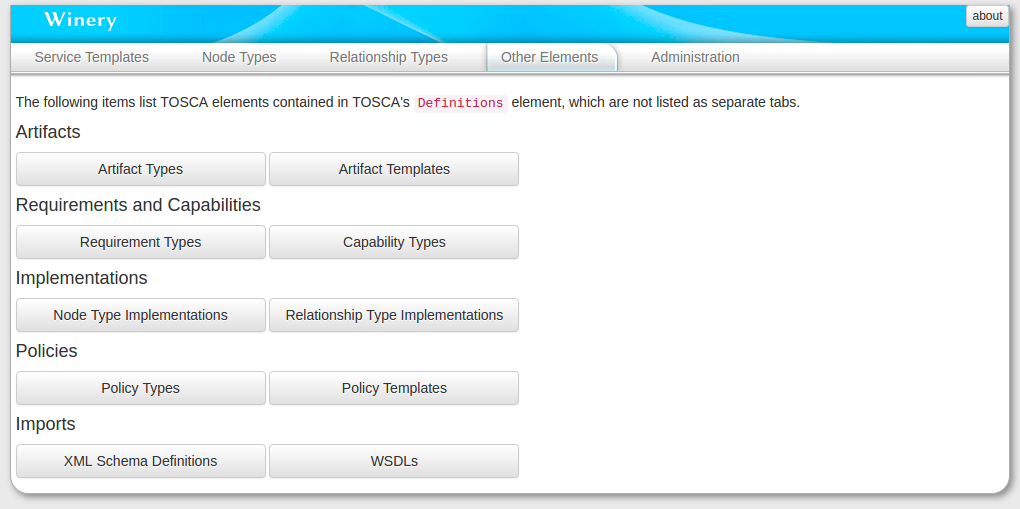
\includegraphics[width=0.7\textwidth]{Screenshot_winery_gui.png}
%	\caption{Visual interface for $Winery$.}
%	\label{fig:winery_gui}
%\end{figure}
\begin{figure}[ht]   
\centering
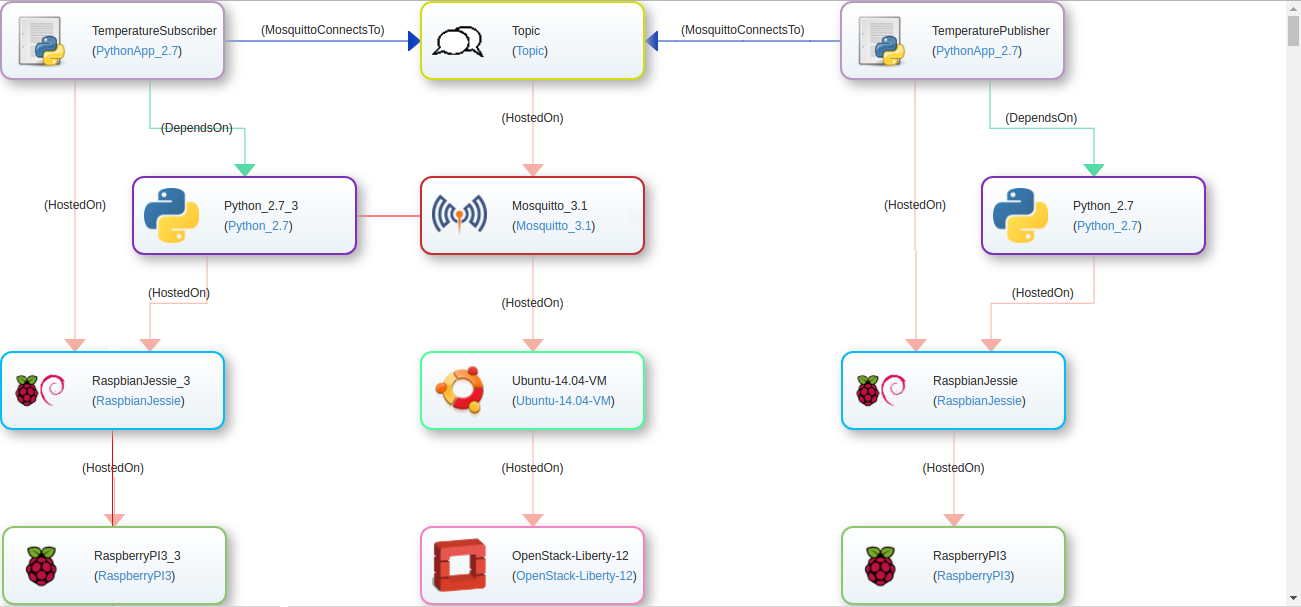
\includegraphics[width=0.7\textwidth]{Screenshot_winery_source.png}
\caption{TOSCA topology visualized by $Winery$.}
\label{fig:winery_source}
\end{figure}
\section{Package Management} \label{sec:pm}
Packages and package management processes are described in this section.
An installation of packages from external source represents an external reference and therefore they will be considered in order to identify such references.
%\subsection*{Package managers}
Package is an archive file containing both data for installation of the program component and a set of metadata like name, function, version, producer, and a list of dependencies to other packages.~\cite*{opium}
These packages can present not only a complete program but also a certain component of a large application. % or libraries, a packages which can be used only by other programs.
For a user, a package manager is a set of software tools which automate the process of installing, updating, configuring and removing packages.
But from the operating system side, a package manager is used for managing the database of packages, their dependencies, and versions, to prevent erroneous installation of programs and missing dependencies.
%\subsection*{Packages}
%\subsection*{Dynamic libraries}
This task is especially complex in computer systems relying on dynamic library linking. 
Those systems share executable libraries of machine instructions across  applications. 
In these systems, complex relationships between different packages requiring different versions of libraries result in a challenge colloquially known as "dependency hell"~\cite*{linuxgeek}.
Good package management is vital to these systems.\\
%\subsection*{Repository}
To give users more control over the kinds of programs that they allow to install on their systems, packages are often downloaded only from a number of software repositories.
In Unix systems, a package manager uses official repositories appropriate for the operating system and the architecture  of device where it's operate, but it's possible to use additional repositories, like third-party repositories or repositories for another architecture.\\
%\subsection*{Dependencies} \label{subs:dep}
Package managers distinguish between two types of dependencies: $required$ and $preRequired$. %\\
Dependency $package1$ \textbf{$required$} $package2$ indicates that the $package2$ must be installed for a proper \textbf{operation} of the $package1$. %\\
Dependency $package1$ \textbf{$preRequired$} $package2$ indicates that the $package2$ must be installed for a proper \textbf{installation} of the $package1$. %\\
%An example for obtaining the dependency list for the Python package is shown in Listing~\ref{lst:dep}.
%\begin{lstlisting}[caption={Example of using $apt$-$cache$ to obtain dependency list for package python}\label{lst:dep},captionpos=t] 
%user@user:~$ apt-cache depends python
%python
%PreDepends: python-minimal
%Depends: python2.7
%Depends: libpython-stdlib
%Conflicts: <python-central>
%Breaks: update-manager-core
%Suggests: python-doc
%Suggests: python-tk
%Replaces: python-dev
%\end{lstlisting}
%\subsection*{Dependency tree}
In these examples, the $package2$ is needed for the $package1$, but the $package2$ itself can require additional packages.
A structure describing all necessary packages and dependencies between them for the given root-package is called a dependency tree. 
The dependency type $required$ can lead to cycles in dependency trees which differs them from the normal tree graph structures.
\subsection*{Example Dependencies Handling}
The $apt$-$get$ package manager will be considered to provide an example of a dependencies handling.
This application is part of \gls{apt} program which uses $dpkg$ application to communicate with an operating system.
The system keeps a database of packages and their condition.
These relations are presented in Figure~\ref{fig:packages}.\\
$apt$-$get$ has many functions: install, remove, update, autoremove, download and so on.
We will consider the install, remove and autoremove operations to present the common algorithms of processing.
When a package manager becomes a $package$ installation command, it builds a dependencies tree for the $package$ and checks the possibility to install these depended packages.
For example, it must check the compatibility with previously installed packages. 
If the check was successful, the $apt$-$get$ downloads and installs the packages starting with the bottom of the tree.
The $package$ is marked in the database as manually installed and all the other packages are marked as automatically installed. 
It will be helpful during the autoremove operation when all automatically installed packages will be checked whether they are still needed.
After installation of packages from the dependencies tree, the $package$ will be ready to work.\\
A $package$ can be deleted during the $remove$ $package$ command.
It happens only if there are no other packages depending on the $package$. 
If the deletion is very important, then these packages can also be removed too to keep the consistency of the database. 
The packages necessary for the $package$ itself will be deleted only by the autoremove command.
% !TeX spellcheck = en_US

% We need layers to draw the block diagram
\usetikzlibrary{calc,positioning}
\usetikzlibrary{arrows.meta}

% Define a few styles and constants
\tikzstyle{entry}=[draw, fill=green!20, minimum height=2.5em]
\tikzstyle{ann} = [above, text width=5em]
\tikzstyle{item} = [entry, text width=7em, shading = axis,rectangle, left color=blue!10!white, right color=blue!30!white,shading angle=135, anchor=north,
minimum height=2em, rounded corners, align=center]
%\def\blockdist{2.3}
%\def\edgedist{2.5}

\begin{figure}
	\centering
\begin{tikzpicture}
\node (aptget) [item] {apt-get};
\node (console) [yshift=+5em, xshift=+5em] at ( aptget) [item] {Console};
\node (script) [yshift=+5em, xshift=-5em] at ( aptget) [item] {Script};
\node (apt) [yshift=-3em] at ( aptget) [item] {APT};
\node (dpkg) [yshift=-3em] at (apt) [item] {dpkg};
\node (system) [yshift=-3em] at (dpkg) [item] {System database};

\draw [->,scale=1,line width=2pt] (console.south) -- (aptget);
\draw [->,scale=2,line width=2pt] (script.south) -- (aptget);
\draw [->,scale=2,line width=2pt] (aptget) -- (apt);
\draw [->,scale=2,line width=2pt] (apt) -- (dpkg);
\draw [->,scale=2,line width=2pt] (dpkg) -- (system);
\end{tikzpicture} 
\caption{Package management} 	\label{fig:packages}
\end{figure}
\section{Configuration Management Tools}
To ease the package management, various tools can be used. 
We will consider some of them to determine the form of files which contains external references.
Usually they are presented by commands in an executable file, which checks an environment and installs the necessary packages using a package manager.
Such files are called scripts and are commonly used.
Popular management tools like Bash, Ansible, Chef and CFEngine will be described below.
\subsection*{Bash} \label{lang:bash}
Bash is a Unix command language written as a free software.
It provides enough capabilities to be used as a  management tool.
In addition Bash denotes a command processor that typically runs in a text window, where a user types commands that cause actions.
Bash is examined because it is very popular since it is the default command line processor in Unix systems~\cite*{bashdef}.
Instead of typing commands direct into a command line, a script can be executed directly.~\cite{bash}
These scripts can be used to configure a system, install package, create files, check environment and so on.
Bash is a very popular and ease language, therefore a huge number of problems have solutions in Bash scripts already.
\subsection*{Ansible} \label{lang:ansible}
Ansible is an open-source automation engine that automates software provisioning, configuration management, and application deployment.
As with most configuration management software, Ansible has two types of servers: controlling machines and nodes.
First, there is a single controlling machine which is where orchestration begins.
Nodes are managed by a controlling machine over SSH.
The controlling machine describes the location of nodes through its inventory.
Ansible playbooks express configurations, deployment, and orchestration in Ansible.
The playbook format is YAML. 
Each playbook maps a group of hosts to a set of roles.
Each role is represented by calls to Ansible tasks.~\cite{ansible} 
\subsection*{Chef} \label{lang:shef}
Chef is a configuration management tool, which uses Ruby for writing system configuration files called "recipes".
They describe how Chef manages applications and utilities and how they are to be configured.
These recipes which can be grouped together as a "cookbook" for easier management define a series of resources that should be in a particular state: packages that should be installed, services that should be running, or files that should be written.
Chef can run in client/server mode, or in a standalone configuration named "chef-solo".
In client/server mode, the Chef client sends various attributes about the node to the Chef server. 
In solo mode the local system will be configured.~\cite{chef}
\subsection*{CFEngine}
CFEngine is an open source configuration management system.
Its primary function is to provide automated configuration and maintenance of large-scale computer systems, including the unified management of servers, desktops, consumer and industrial devices, embedded networked devices, mobile smartphones, and tablet computers.~\cite{cfengine}
Configurations are described by "policy" files, which are plain text-files with .cf extension.
These files define the necessary state of files, packages, users, processes, services and so on.~\cite{cfengine2}

% !TeX spellcheck = en_US

\chapter{Requirements}
\label{chap:req}
Since the main purpose of the developed framework is to Resolve References, further the $RR$ can be used as an abbreviation. 
$RR$ should eliminate external dependencies in a TOSCA topology represented by a CSAR file.
$RR$ must be easily extendable to provide the ability to eliminate a large number of dependency types.\\
As a first step, a minimal configuration which handles $Bash$ language with the $apt$-$get$ package manager and $Ansible$ language with the $apt$ package manager will be developed. 
These software handlers of languages and package managers will be called language modules and package manager modules.
As an example, the $Bash$ and $apt$-$get$ modules will remove package installation commands from bash-scripts ($apt$-$get$ $install$ \textbf{$package$}).
Then both the \textbf{$package$} itself and all the depended packages from his dependencies tree will be downloaded.
It is also necessary to update the topology of the TOSCA, by adding new nodes and dependencies.
To do so, common definitions will be added, like Relationship Types and Artifact Types.
 % for downloaded packages and dependencies from nodes previously containing an external reference to the node displaying the downloaded packages. 
Then new nodes will be defined by Node Types, Node Type Implementations, Artifacts Templates, and instantiated by Node Templates. 
Relations between nodes will be instantiated by Relationship Templates.
These Templates must be added to the right Service templates, where the nodes containing external references are instantiated.
%Dependencies between downloaded packages, representing dependency tree should be added too.
To find the Service Templates and Node Types corresponding to a certain artifact, it can be useful to apply preprocessing to the entire TOSCA topology. \\
%References chain can be build:\\
%$script$ $\rightarrow$ $Artifact$ $Implementation$ $\rightarrow$ $Node$ $Type$ $Implementation$ $\rightarrow$ $Node$ $Type$ $\rightarrow$ $Node$ $Template$ $\rightarrow$ $Service$ $Template$\\
After implementing the minimal configuration, it should be easy to add more language modules and package manager modules, like $Aptitude$ for Bash or completely new language like $Chef$.
In order to proof the correctness of the corresponding TOSCA topology, Winery described in section \ref{tool:winery} will be used.
\section*{Stages of the processing}
Here an example is provided, representing how the framework should work.
\begin{itemize}  
	\item Begin  \\
%	To start the work $RR$ needs input CSAR name, output CSAR name, and architecture of target hardware. 
%	This will be done using user input.
	An input CSAR will be extracted.
	\item Preprocessing\\
	During preprocessing stage, RR needs to analyze internal references.
	In additional, common Tosca definitions for artifacts and relations between packages will be added.
	\item Processing with language modules\\
	Each file from the input CSAR will be processed by Language modules.
	\item Processing with packet manager modules\\
    If the file belongs to an Language, it will be processed by the packet manager module belonging to the Language to find and resolve external references.
    Package name from this reference will be moved forward.
	\item Package handling\\
	Using the package name the package will be downloaded and TOSCA definitions created. These actions will be recursively repeated for all dependent packages, creating the dependency tree in the TOSCA topology.
	\item Topology handling\\
	Using information about internal references and dependencies the TOSCA Topology will be updated by creating new Node and Reference Templates. 
	\item End\\
	Meta-file should be updated and all data packed back to the CSAR.
\end{itemize}
These steps will be represented by the modules described in section \ref{sec:arch} and implemented in chapter \ref{chap:imp}.

\section*{Result}
As a result of the work, an output CSAR will be received. 
This CSAR must have the same functionality as the input CSAR, but all external references to additional packages must be resolved.
The output CSAR must be able to be deployed properly without downloading these packages over the Internet. 
In additional, the topology for the packages must be mirrored from the package manager's database to the TOSCA topology.
% !TeX spellcheck = en_US

\chapter{Concept and Architecture}\label{chap:conarch}
In this chapter, the concept and the architecture of the framework, which can satisfy the requirements will be described and substantiated.
Solutions to some additional problems will be presented. 
\section{Concept}
In this section, the main concept of this work will be described.
The general structure of the framework is represented in the block diagram \ref{fig:gen}. 
In the section~\ref{subs:analyse}, it will be found out how to determine during the preprocessing stage which Node Templates uses the given artifact.
Then a functionality of language modules and package manager modules is described.
In the section~\ref{subs:repres}, it will be explained how to create a new node for a TOSCA topology. 
After that, a problem of the determining the architecture of the final platform will be explained and a solution described.
In additional, it will be described, how the results can be validated.
% !TeX spellcheck = en_US

\begin{figure}
	\centering
\begin{tikzpicture}
\node[draw] (in) at (0,1.5) {Input CSAR};
\node[draw] (pp) at (0,+0.5) {Preprocessing};
\node[draw] (lm) at (0,-0.5) {Language modules};
\node[draw] (pmm) at (-3,-2) {Package manager modules};
\node[draw] (dtm) at (+3,-2) {Download tool modules};
\node[draw] (ph) at (-1.5,-3) {Package handler};
\node[draw] (th) at (0,-4) {Topology handler};
\node[draw] (out) at (0,-5) {Output CSAR};
\draw [->] (in) -- (pp);
\draw [->] (pp) -- (lm);
\draw [->] (lm) -- (pmm);
\draw [->] (lm) -- (dtm);
\draw [->] (pmm) -- (ph);
\draw [->] (dtm) -- (th);
\draw [->] (ph) -- (th);
\draw [->] (th) -- (out);
\end{tikzpicture} 
\caption{The general description of the software's work flow} 	\label{fig:gen}
\end{figure}


\subsection{Analysis existing TOSCA-Topology}\label{subs:analyse}
To properly update the \gls{tosca} topology, it is necessary to add references from the nodes where external references were to newly created nodes, which resolve the external references. 
According to the TOSCA standard, only references between Node Templates in the same Service Template can be created.  
That means that each Node Template, which uses artifacts with external references must be found.
Furthermore, Service Template where these Node Templates are instantiated must be found to create there a Node Template for the new nodes and reference them to the Node Templates with external references.
The Pointers to Artifacts are contained by Artifact Templates, which are used by Node Type Implementations.
By composing all the information a simple references chain can be built:\\
$Artifact$ $\rightarrow$ $Artifact$~$Template$ $\rightarrow$ $Node$~$Type$~$Implementation$ $\rightarrow$ $Node$~$Type$ $\rightarrow$ $Node$~$Template$ $\rightarrow$ $Service$~$Template$\\
Now consider the references in more detail. 
\begin{itemize}
	\item $Artifact$ $\rightarrow$ $Artifact$ $Template$\\
	An Artifact can be referenced by several Artifact Templates. (Despite the fact that this is a bad practice.)
	\item  $Artifact$ $Template$ $\rightarrow$ $Node$ $Type$ $Implementation$ \\
	The same way an Artifact Template can be used by several Node Type Implementations.
	\item $Node$ $Type$ $Implementation$ $\rightarrow$ $Node$ $Type$ \\
	A Node Type Implementation can describe an implementation of only one Node Type.
	\item  $Node$ $Type$ $\rightarrow$ $Node$ $Template$\\
	Each Node Type can have any number of Node Templates.
	\item  $Node$ $Template$ $\rightarrow$ $Service$ $Template$\\
	But each Node Template is instantiated only once.
\end{itemize}
Thus structure can be described by a tree with an Artifact as the root, and Service Templates as leaves (The example is on figure \ref{fig:script_serv}) and will be called the internal dependencies tree.
% !TeX spellcheck = en_US
\usetikzlibrary{calc,arrows.meta,positioning}
\tikzset{
    every node/.style={font=\sffamily\small},
    main node/.style={shape=rectangle, rounded corners,
    	draw, align=center,
    	top color=white, bottom color=blue!20}
}

\begin{figure}
	\centering
\begin{tikzpicture}[sibling distance=14em,->,>={Stealth[round,sep]},shorten >=1pt,auto,node distance=25mm]
    \node[main node] (1) {Script}
    child { node[main node](3) {Artifact Implementation 1} 
    	child { node[main node] (6) {Node Type Implementation 1} 
    			child { node[main node] (8) {Node Type 1} 
    				child { node[main node]  (11) {Node Template 1} 
    					child { node[main node] (13) {Service Template 1}}  
    				}
    				child { node[main node]  (12) {Node Template N} 
    					child { node[main node] (14) {Service Template N}}
    				}
    			}
    	}
    	child { node[main node] (7) {Node Type Implementation N} 
    		child { node[main node] (9) {Node Type N} 
    			child { node  (10) {\ldots} }
    		}
    	}
    }
    child { node[main node] (4) {Artifact Implementation N}  
    child { node (5) [below =of 4]{\ldots}}
	};

    \node at ($(3)!.5!(4)$) {\ldots};
    \node at ($(6)!.5!(7)$) {\ldots};
    \node at ($(11)!.5!(12)$) {\ldots};
    
\end{tikzpicture} 
\caption{Example tree describing how to find Service Templates and Node Templates for a given script} 	\label{fig:script_serv}
\end{figure}
%Of course it is possible to move in opposite direction, starting from a Node and moving toward scripts, but this method brings additional complexity. 
An additional problem is in the reference between a Node Type and a Node Type Implementation.
Node Type can have several implementations, but which one will be used will be determined only during the deployment. 
The chosen solution to this problem is to use each Node Type Implementation in hope, that they will not conflict.\\
%The method presented above can uniquely determine Node Templates and Service Template for a given script.
%Of course it is not guaranteed that found Node Type Implementation will be used during deployment, but we can't do anything with this. 
The following steps can be executed during the preprocessing, to build the internal dependencies tree.
\begin{itemize}
	\item Find all Artifact Templates to build references from Artifacts to Artifact Templates.
	\item Find all Node Type Implementations. Because they contain references both to the Node Type and to the Artifact Templates, then the dependency from Artifact to Node Types can be built.
	\item Find all Service Templates and in them contained Node Templates. Each Node Template contains a reference to Node Type, what is useful for building a dependency from Artifact to Node Template.
\end{itemize} 
In this way, the required internal dependencies tree can be built (with references $Artifact$ $\rightarrow$ $Node$~$Template$ and $Artifact$ $\rightarrow$ $Service$~$Template$).

\subsection{Modules and extensibility}
Unfortunately, it is impossible to identify all types of external references, even when only one language and one package manager are used (an example in the listing \ref{alg:unreadable}).
\begin{Listing} 
	\caption{Unreadable bash script}
	\label{alg:unreadable}
\begin{lstlisting}
#!/bin/bash
set  line = abcdefgijklmnoprst
set  word1 = ${line:0:1}${line:14:1}${line:17:1} 
set  word2 = ${line:6:1}${line:4:1}${line:17:1}
$word1-$word2 install package
\end{lstlisting}
\end{Listing}
Since this work is aimed at creating of the easily expanded and supplemented tool, initially only basic usage of package managers will be considered.\\
The framework should handle different languages, each of them can support various package managers.
A language module should filter files not belonging to the language, and accepted files will be transmitted to corresponding package manager modules.
This principle can be illustrated by a figure \ref{fig:lang_pm}.
% !TeX spellcheck = en_US

% We need layers to draw the block diagram
\usetikzlibrary{calc,positioning}

% Define a few styles and constants
\tikzstyle{entry}=[draw, fill=green!20, minimum height=2.5em]
\tikzstyle{ann} = [above, text width=5em]
\tikzstyle{framework} = [entry, text width=35em, fill=red!20, 
minimum height=18em, rounded corners]
\tikzstyle{lang} = [entry, text width=9em, fill=blue!20, 
minimum height=15em, rounded corners]
\def\blockdist{2.3}
\def\edgedist{2.5}

\begin{figure}
	\centering
\begin{tikzpicture}
\node (rr) [framework] {};
\node [xshift=+5mm, yshift=-2mm, below right] at (rr.north west) {\large References resolver Framework };


\node (lang1) at ([xshift=-52mm,yshift=-4mm]rr) [lang] {};
\node [xshift=+3mm, yshift=-2mm, below right] at (lang1.north west) {\large Language 1 };
\node (lang2) at ([xshift=-7mm,yshift=-4mm]rr) [lang] {};
\node [xshift=+3mm, yshift=-2mm, below right] at (lang2.north west) {\large Language 2 };
\node (langn) at ([xshift=+52mm,yshift=-4mm]rr) [lang] {};
\node [xshift=+3mm, yshift=-2mm, below right] at (langn.north west) {\large Language N };
\node at ($(lang2)!.5!(langn)$) {\ldots};

\node (l1pm1) at ([yshift=+15mm]lang1) [entry] {Package manager 1};
\node (l1pm2) at ([yshift=0mm]lang1) [entry] {Package manager 2};
\node (l1pmn) at ([yshift=-22mm]lang1) [entry] {Package manager K};
\node at ($(l1pm2)!.5!(l1pmn)$) {\vdots};

\node (l2pm1) at ([yshift=+15mm]lang2) [entry] {Package manager 1};
\node (l2pm2) at ([yshift=0mm]lang2) [entry] {Package manager 2};
\node (l2pmn) at ([yshift=-22mm]lang2) [entry] {Package manager L};
\node at ($(l2pm2)!.5!(l2pmn)$) {\vdots};

\node (lnpm1) at ([yshift=+15mm]langn) [entry] {Package manager 1};
\node (lnpm2) at ([yshift=0mm]langn) [entry] {Package manager 2};
\node (lnpmn) at ([yshift=-22mm]langn) [entry] {Package manager M};
\node at ($(lnpm2)!.5!(lnpmn)$) {\vdots};


\end{tikzpicture} 
\caption{Example scheme representing several languages and package managers} 	\label{fig:lang_pm}
\end{figure}
A package manager module resolves an external reference and transmits the package name to a package handler, described in section \ref{subs:archph}.\\
The framework will contain a list of all supported language modules, and each language module will contain a list of supported package managers modules.
Ease of adding new modules to the framework will proof the correctness of the architecture.\\
At the beginning, the most popular combination will be implemented: the $bash$ language with the $apt-get$ package manager.
This simple and powerful tool allows to install, delete or update the set of packages in one line.
A line-by-line parser should be developed, which analyses scripts and finds the installation commands.
After the modules for this combination will be implemented, new language and package manager modules should be added.

\subsection{Representing downloaded packages in TOSCA-Topology} \label{subs:repres}
A package node denotes to the defined and instantiated element of \gls{tosca} topology, the purpose of which is to install the package.
The adding of new package nodes to TOSCA topology can be divided into several steps.
\begin{itemize}
	\item Add definitions for common elements, like Artifact Types or Relationship Types. 
		This can be done once at the preprocessing stage.
	\item The package node main definition will be represented by a Node Type. 
		%There will be described that this node must be installed.
	\item Artifacts (The downloaded data and the installation script) will be referenced by Artifact Templates.
	\item Node Type Implementation will combine the artifacts.
	\item Node Template will instantiate the package node in the corresponding Service Templates.
		To determine corresponding Service Template the preprocessing described in the section \nameref{subs:analyse} will be used.
	\item Reference Template will provide topology information, allowing the observer (a user or a runtime environment) to determine, for which nodes the package must be installed.
		References will be created from the Node Template needing the package to Node Template of created package nodes.
\end{itemize}
After an execution of those steps, a definition of a package node will be finished and this node can be used.
\subsection{Determining architecture of a final platform}
An another problem appears during choosing the architecture of the device where packages will be installed.
Unfortunately, it is impossible to analyze the structure of any CSAR and give an unambiguous answer to the question, on which architecture which node will be deployed.
There are many pitfalls here.\\
A single Service Template can use several physical devices with different architectures.
One Implementation Artifacts can be referred by different Node Types and Node Templates, instantiated on different platforms.
This way one simple Implementation Artifact with a bash script containing "$apt$-$get$ $install$ $python$" command can be deployed on different devices within one Service Template (for example with the arm, amd64 and i386 architectures) and will result in the loading and installation of three different packages. 
For an end user, the ability to use such a simple command is a huge advantage, but for the framework, it can greatly complicate analysis.
The following methods of architecture selection were designed.
\begin{itemize}
	\item $Deployment$ $environment$ $analysis$\\
	The script can analyze the system where it was started (for example using the "$uname$~$-a$" command) and depending on the result, it will install the package corresponding to the system's architecture.
	\item $Unified$ $architecture$\\
	The architecture will be defined by the user for a whole CSAR.
	\item $Artifact$ $specific$ $architecture$\\
	The architecture will be defined separately for each artifact.
\end{itemize}
\subsubsection*{Analysis of methods}
The $deployment$ $environment$ $analysis$, which at first sight seems to be the most reliable solution, brings many additional problems.
Packages for different platforms can differ not only by architecture but also by the version and the list of dependencies.
As a consequence, a chaos can be produced by mirroring these different packages with different versions to the \gls{tosca}-topology.
The only robust solution seems to be to create for each installed package a set of archives (one archive for one architecture), containing the entire dependency tree for the given package.
But this approach contradicts one of the main ideas of this work: the dependencies trees should be mapped to the topology.\\
The $artifact$ $specific$ $architecture$ method carries an additional complexity to the user of the framework.
It will obligate a user to analyze each artifact and decide on which architecture it will be executed. 
This can be complicated by the fact that the same artifact can be executed on different architectures.\\
The method of the $unified$ $architecture$ was chosen, as the simplest and easiest to implement.
If it will be necessary, this method can be easily expanded to the $artifact$ $specific$ $architectures$ method (By removing the user input at start, and choosing an architecture for each artifact separately.) or to $deployment$ $environment$ $analysis$ (By downloading packages for all available architectures and adding the architecture determining algorithm to the installation scripts.).

%\subsection{Extensibility}
%The framework should handle different languages, each of them can support various package managers.
%An language module should filter files not belonging to the language, accepted files will be processed 
%This principle can be illustrated by a figure \ref{fig:lang_pm}.
%% !TeX spellcheck = en_US

% We need layers to draw the block diagram
\usetikzlibrary{calc,positioning}

% Define a few styles and constants
\tikzstyle{entry}=[draw, fill=green!20, minimum height=2.5em]
\tikzstyle{ann} = [above, text width=5em]
\tikzstyle{framework} = [entry, text width=35em, fill=red!20, 
minimum height=18em, rounded corners]
\tikzstyle{lang} = [entry, text width=9em, fill=blue!20, 
minimum height=15em, rounded corners]
\def\blockdist{2.3}
\def\edgedist{2.5}

\begin{figure}
	\centering
\begin{tikzpicture}
\node (rr) [framework] {};
\node [xshift=+5mm, yshift=-2mm, below right] at (rr.north west) {\large References resolver Framework };


\node (lang1) at ([xshift=-52mm,yshift=-4mm]rr) [lang] {};
\node [xshift=+3mm, yshift=-2mm, below right] at (lang1.north west) {\large Language 1 };
\node (lang2) at ([xshift=-7mm,yshift=-4mm]rr) [lang] {};
\node [xshift=+3mm, yshift=-2mm, below right] at (lang2.north west) {\large Language 2 };
\node (langn) at ([xshift=+52mm,yshift=-4mm]rr) [lang] {};
\node [xshift=+3mm, yshift=-2mm, below right] at (langn.north west) {\large Language N };
\node at ($(lang2)!.5!(langn)$) {\ldots};

\node (l1pm1) at ([yshift=+15mm]lang1) [entry] {Package manager 1};
\node (l1pm2) at ([yshift=0mm]lang1) [entry] {Package manager 2};
\node (l1pmn) at ([yshift=-22mm]lang1) [entry] {Package manager K};
\node at ($(l1pm2)!.5!(l1pmn)$) {\vdots};

\node (l2pm1) at ([yshift=+15mm]lang2) [entry] {Package manager 1};
\node (l2pm2) at ([yshift=0mm]lang2) [entry] {Package manager 2};
\node (l2pmn) at ([yshift=-22mm]lang2) [entry] {Package manager L};
\node at ($(l2pm2)!.5!(l2pmn)$) {\vdots};

\node (lnpm1) at ([yshift=+15mm]langn) [entry] {Package manager 1};
\node (lnpm2) at ([yshift=0mm]langn) [entry] {Package manager 2};
\node (lnpmn) at ([yshift=-22mm]langn) [entry] {Package manager M};
\node at ($(lnpm2)!.5!(lnpmn)$) {\vdots};


\end{tikzpicture} 
\caption{Example scheme representing several languages and package managers} 	\label{fig:lang_pm}
\end{figure}

\subsection{Result's checking}
Checking the output of the framework is an important stage in the development of the program.
It is necessary to verify both the overall validity of the output \gls{csar} and the possibility to deploy generated package nodes.
To test for overall correctness it is possible to use $winery$ tool from OpenTOSCA.
This tool for creating and editing CSAR archives is also great for visualizing the results.
Checking the deployment of the generated package nodes can be done manually by entering commands starting the implementation artifact's execution.

\section{Architecture}\label{sec:arch}
This section will present the architecture of the framework and the detailed description of its elements.
The main elements are a $CSAR$ $handler$, a $references$ $resolver$, $language$ $modules$, $package$ $manager$ $modules$, a $package$ $handler$, and a $topology$ $handler$.

\subsection{CSAR handler} \label{subs:casr_h}
The CSAR handler provides an access to a \gls{csar} and maintains it's consistency. 
It describes the processes of the adding of new files (to handle the metadata), archiving/unarchiving, and the choosing of a final platform architecture.

\subsection{References resolver} \label{subs:RR}
This is the main element, the execution of which can be divided into the three stages: $preprocessing$, $processing$, $finishing$. \\
During the $preprocessing$ stage, the CSAR will be unarchived, common files added, and internal dependencies trees generated.
Figure \ref{fig:preproc} illustrates those steps.
During the $processing$, all $language$ $modules$ will be activated, which are described in more details in the next section. \\
To finish the work all results will be packed to the output CSAR during the $finishing$ stage.
% !TeX spellcheck = en_US

\usetikzlibrary{calc,arrows.meta,positioning,arrows}
\tikzset{
    every node/.style={font=\sffamily\small},
    main node/.style={shape=rectangle, rounded corners,
    	draw, align=center,
    	top color=white, bottom color=blue!20}
}

\tikzstyle{entry}=[draw, fill=green!20, minimum height=2.2em, text width=7em]
\tikzstyle{myentry}=[draw, fill=Dandelion!20, minimum height=2.5em, text width=7em]
\tikzstyle{ann} = [above, text width=5em]
\tikzstyle{frame} = [entry, text width=9em, fill=red!20, 
minimum height=17em, rounded corners]
\tikzstyle{csar_content} = [entry, text width=8em, fill=blue!20, 
minimum height=14em, rounded corners]
\def\blockdist{2.3}
\def\edgedist{2.5}
\begin{figure}
	\centering
\begin{tikzpicture}[sibling distance=9em,->,>={Stealth[round,sep]},shorten >=1pt,auto,node distance=25mm]


\node (csar_frame) [frame] {};
\node [xshift=+5mm, yshift=-2mm, below right] at (csar_frame.north west) {\large CSAR};

\node (csar_content) at ( [yshift=-3mm]csar_frame) [csar_content] {};
\node [xshift=+5mm, yshift=-2mm, below right] at (csar_content.north west) {\large content};

\node (l2pm1) at ([yshift=+15mm]csar_content) [entry] {Definitions\\};
\node (l2pm2) at ([yshift=0mm]csar_content) [entry] {TOSCA-Metadata\\};
\node (l2pmn) at ([yshift=-22mm]csar_content) [entry] {Artifacts\\};
\node at ($(l2pm2)!.5!(l2pmn)$) {\vdots};
    
\node [right of=csar_frame, xshift=30mm](dc_frame) [csar_content] {};
\node [xshift=+1mm, yshift=-2mm, below right] at (dc_frame.north west) {\large Decompressed};
\draw [->] (csar_frame) -- (dc_frame);
\node (2pm1) at ([yshift=+15mm]dc_frame) [entry] {Definitions\\};
\node (2pm2) at ([yshift=0mm]dc_frame) [entry] {TOSCA-Metadata\\};
\node (2pmn) at ([yshift=-22mm]dc_frame) [entry] {Artifacts\\};
\node at ($(2pm2)!.5!(2pmn)$) {\vdots};

\node [right of=dc_frame, xshift=30mm](my_frame) [frame] {};
\node [xshift=+5mm, yshift=-2mm, below right] at (my_frame.north west) {\large With my files};
\draw [->] (dc_frame) -- (my_frame);
\node (3pmd) at ([yshift=+20mm]my_frame) [myentry] {My definitions\\};
\node (3pm1) at ([yshift=+6mm]my_frame) [entry] {Definitions\\};
\node (3pm2) at ([yshift=-8mm]my_frame) [entry] {TOSCA-Metadata\\};
\node (3pmn) at ([yshift=-28mm]my_frame) [entry] {Artifacts\\};
\node at ($(3pm2)!.5!(3pmn)$) {\vdots};


\node[below=of dc_frame,main node, node distance=10mm, xshift=-4mm, yshift=+7mm] (11) {Script 2}
child { node[main node, yshift=-10mm]  (n21) {Node Template 1} 
		child { node[main node] (s31) {Service Template 1}}  
}
child { node[main node, yshift=-10mm]  (n22) {Node Template N} 
	child { node[main node] (s32) {Service Template N}}  
};
\draw [dashed,->] (dc_frame) -- (11);
\node[below left=of dc_frame,main node,xshift=+10mm] (12) {Script 1}
child { node  {\ldots} 
};
\draw [dashed,->] (dc_frame) -- (12);
\node[below right=of dc_frame,main node, xshift=-10mm] (13) {Script K}
child { node  {\ldots} 
};
\draw [dashed,->] (dc_frame) -- (13);
\node at ($(11)!.5!(13)$) {\ldots};
\node at ($(n21)!.5!(n22)$) {\ldots};

\end{tikzpicture} 
\caption{Preprocessing: decompression, adding files and generating dependencies} 	\label{fig:preproc}
\end{figure}

\subsection{Language modules} \label{subs:archlm}
Each $language$ $module$ describes a handling of one language and chooses files written in the language.
It also contains a list of supported package manager modules.
Each language module must provide the capability to generate a TOSCA node for a given package and this node must use the same language to install the package.
That means, that a script and definitions for Artifact Templates, a Node Type, and a Node Type Implementation should be created by a language module.\\
As already mentioned above, during $processing$ stage a $language$ $module$ analyzes all files one by one and checks their belonging to the language. 
Any files not belonging to the described language are filtered out.
The remaining files are transferred to the $language$ $module$'s $package$ $manager$ $modules$.
For example, a $bash$ module will pass only files with $".sh"$ extension, which start with the $"\#!/bin/bash"$ line.
An $ansible$ module should have an additional functionality to unpack zip archives, where ansible playbooks can be stored.
Since ansible playbooks don't contain specific header or marker, the single sigh of ansible files is the "$.yml$" extension. 

\subsection{Package manager modules} \label{subs:archpmm}
A $package$ $managers$ $module$ finds external references, resolves them and transmits the package name to the $package$ $handler$, described in the next section.
Figure \ref{fig:lang_ph} illustrates data flow between language modules, package manager modules, and the package handler.\\
To resolve an external reference a package manager module will parse a given file. 
In the case of the apt-get module for bash, the module will read a file line-by-line searching for the strings starting with "apt-get install".
Such strings must be commented out and those ends should be divided to separate package names, which will be transferred to the package handler. 
% !TeX spellcheck = en_US
\usetikzlibrary{calc,arrows.meta,positioning}
\tikzset{
    every node/.style={font=\sffamily\small},
    main node/.style={shape=rectangle, rounded corners,
    	draw, align=center,
    	top color=white, bottom color=blue!20},
    data node/.style={shape=rectangle,
    draw, align=center,
    top color=white, bottom color=red!20}
}

\begin{figure}
	\centering
\begin{tikzpicture}[->,>={Stealth[round,sep]},shorten >=1pt,auto,level 1/.style={sibling distance=10em,node distance=25mm},
level 2/.style={sibling distance=8em,node distance=30mm},
level 3/.style={sibling distance=12em,node distance=30mm},
level 4/.style={sibling distance=6em,node distance=25mm},
level 5/.style={sibling distance=8em,node distance=25mm},
level 6/.style={sibling distance=8em,node distance=25mm}]
    \node[data node] (1)  {All files from original CSAR}
    child { node[main node](2) {Language 1} 
    	child { node[data node](21) {Files accepted by\\ Language 1} 
    		child { node {\ldots}}}}
	child { node[main node] (3) {Language 2}
		child { node[data node](31) {Files accepted by\\ Language 2} 
			child { node[main node, yshift=-13mm](32) {Package manager 1\\for Language 2} 
				child { node[data node](36) {Updated\\ files}}
				child { node[data node](37) {Package\\ names}}}
			child { node[main node, yshift=-13mm, xshift=-3mm](33) {Package manager 2\\for Language 2}
				child { node[data node](34) {Updated\\ files}}
				child { node[data node](35) {Package\\ names}}}
			child { node[main node, yshift=-13mm, xshift=+3mm](34) {Package manager K\\for Language 2}
				child { node[data node](38) {Updated\\ files}}
				child { node[data node](39) {Package\\ names}}}
			}
		}
    child { node[main node] (4) {Language N}
    	child { node[data node](41) {Files accepted by\\ Language N} 
    		child { node {\ldots}}}}
	;

	\node [main node,below, yshift=-20mm] at (35) (ph) {Package handler};
    \node at ($(3)!.5!(4)$) {\ldots};
    \node at ($(33)!.5!(34)$) {\ldots};
    \draw [->] (35) --(ph);
    \draw [->] (37) --(ph);
    \draw [->] (39) --(ph);
    
\end{tikzpicture} 
\caption{Data flow scheme between language modules, package manager modules and package handler.} 	\label{fig:lang_ph}
\end{figure}

\subsection{Package Handler} \label{subs:archph}
The $package$ $handler$ becomes a package name, downloads an installation data for an architecture specified by the CSAR handler, transfers the package name to the $topology$ $handler$ and recursively repeats the actions for all depended packages. 
To download an installation data the command "apt-get download \textbf{package}" can be used. 
The architecture can be specified by a ":$architecture$" suffix, for example, a "package:$arm$" mean the package of the $arm$ architecture.
The list of dependencies will be obtained using the "apt-cache depends \textbf{package}" command. 
The output of such command should be parsed in order to extract names of depended packages.
Of course, in a case of a fault during a download of a package, a user interface should be provided, to find a solution.
That can be: retry the download, ignore the package, rename the package, or even break the framework's execution.

\subsection{Topology Handler} \label{subs:archtop}
This element should handle the TOSCA topology and has two main tasks: analyze the TOSCA topology during the preprocessing stage to create internal dependencies tries and use those tries to create TOSCA definitions for Node Templates and Relationship Templates in right places for packages provided by the package handler.
The analyze of the TOSCA topology was described in the section \ref{subs:analyse} and the defining of Node Templates and Relationship Templates in the section \ref{subs:repres}.
%$Topology$ $handler$ adds a package to the topology. 
%This includes adding new files and updating existing files. 
%Necessary steps were described in section \ref{subs:repres}.
% !TeX spellcheck = en_US

\chapter{Implementation}\label{chap:imp}
This chapter provides an information about the implementation of the framework and its elements, whose behavior was described in chapter \ref{chap:conarch}.
Java language was chosen, because of its simplicity and strength. 
In this language, the elements are represented by classes.
Java uses additional kind of packages which describe third-party modules and make programming easier. 
The used Java packages will be mentioned here and the necessary license will be listed in the "NOTICE.txt" file in the source code's root folder.

\section{Global elements}
This section describes the elements used throughout the whole framework's execution.
A ZIP handler provides a functionality to operate ZIP archives, a CSAR handler keeps an interface to interact with a CSAR and a Utils helps to solve problems common to other elements.

\subsection*{Zip handler}
This is a small element with straight functionality. 
It serves to pack and unpack ZIP archives which are used by the CSAR standard.
It was decided to use the $java$.$utils$.$zip$ package for this task.
The functions of archiving and unarchiving are called $zipIt$ and $unZipIt$ respectively. 

\subsection*{CSAR handler}
This element provides an interface to access the CSAR content and stores information about files associated with it.
The most valuable data are the name of a temporary extraction folder, the list of files from the input CSAR, the meta-file entry, and the architecture of the target platform.
All this data is encapsulated into the CSAR handler.
The set of public functions allowing to operate with this element is available.
\begin{itemize}
	\item $unpack$ and $pack$ functions are used to extract the CSAR into the temporary folder and pack the folder to the output CSAR. 
	These functions use the $ZIP$~$handler$.
	\item $getFiles$ returns the list with files presented by the input CSAR.
	\item $getFolder$ returns the path to the folder where the CSAR was extracted.
	\item $getArchitecture$ returns the chosen architecture of the target platform.
	\item $addFileToMeta$ adds information about the new file to the meta-data.
\end{itemize}
Here is an example usage of the element.
When the CSAR handler extracts the input CSAR to the temporary extraction folder during the $unpack$'s call, it saves the folder's name. 
Then other elements can use the $getFolder$ function to get this name and access the data.

\subsection*{Utils}
This class provides the $createFile$, $getPathLength$, and $correctName$ methods used by many other elements.
The main purpose of these functions is to make the code cleaner. \\
Using the $createFile$ an element can create a file with the given content.
The $getPathLength$ function returns the deep of the given file's path and it is very useful for creating references between files.\\
The OpenTOSCA uses some limitations to names of TOSCA nodes. 
Those names can't contain slashes, dots and so on.
To obtain an acceptable name from a given name the function $correctName$ can be used.

\section{References resolver}
This is the main module which starts by framework startup and is executed into three stages: preprocessing, processing and finishing.

\subsection*{Preprocessing}
At the preprocessing stage, the CSAR is unpacked, common \gls{tosca} definitions are generated and internal dependencies trees are built. 
%
%\subsubsection*{Unpacking}
To unpack the CSAR the function $unpack$ from the CSAR handler is used.\\
%
%\subsubsection*{Generating TOSCA Definitions}
The $javax$.$xml$.$bind$ package was chosen for creating the common TOSCA definition. 
This Java package allows to generate a description - Java class describing an XML document. 
Those documents contain the following definitions.
\begin{itemize}
	\item $DependsOn$ and $PreDependsOn$ describe Relationship Types %(Described in the section \nameref{subs:reltype})
	  between packages.% (described in the section \nameref{subs:dep}). 
	\item $Package$ $Artifact$ defines a deployment Artifact Type for a package installation data.
	\item $Script$ $Artifact$ specify an implementation Artifact Type for a script installing a package.
	\item $Ansible$ $Playbook$ represent a deployment Artifact Type for a package installation via an ansible playbook.
\end{itemize}
An example description of the $Script$ $Artifact$ can be found in listing~\ref{lst:scripttype}.
Each description is represented by a separate Java class.\\
%
%\subsubsection*{Build internal dependencies trees}\label{subs:imp_findintref}
%Internal dependencies are mainly used by the \nameref{subs:archtop}.
%Therefore, these two modules were combined within the one Java class named $Topology$~$Handler$.
To build internal dependencies trees the topology handler described in section \ref{sec:imptophan} is used. 

\subsection*{Processing}
During this stage, all language modules listed in the framework are started.
For the references resolver element that is only two strings of code, but they start the main functionality of the framework.
%Since the language modules are stored in $language$ variable, this simple stage can be presented by the listing~\ref{lst:start_lang}.
%\begin{Listing}
%\caption{The processing stage}
%\label{lst:start_lang}
%\begin{lstlisting}
%for (Language l : languages)
%	l.proceed(cr);
%\end{lstlisting}
%\end{Listing}


\subsection*{Finishing}
To finish the work the changed data should be packed back into a \gls{csar}.
The function $pack$ from the CSAR handler is used. 

\section{Language modules} 
This section will describe the language modules. %implementation of %TODO
%For this purpose serve \nameref{subs:archlm} and \nameref{subs:archpmm}.
Since the framework is initially oriented to easy extensibility, an abstract model for the modules will be defined, so that new modules can be added by implementing this model.
The implementation of the bash and ansible modules will be provided at the end of the section.

\subsection*{Language model}
To specify the common functionality and behavior of different language modules, the language model is used. 
In Java, this model is described by an abstract class. 
The abstract class $Language$ is presented in listing~\ref{lst:langabst}.
The common variables for all language modules are the name of the language, the list with package manager modules, and the extensions of files.
And here are the common functions presented: 
\begin{itemize}
	\item $getName$ returns the name of this language.
	\item $getExtensions$ returns the list of extensions for this language.
	\item $proceed$ checks all original files.  
	Files written in the language should be transferred to every supported package manager module.
	\item $getNodeName$ uses a package name to generate the name for a Node Type, which will install the package using this language.
	\item $createTOSCA\_Node$ creates the definitions for a TOSCA node. 
	Since the created TOSCA nodes must install packages using the same language as the original node, all languages must provide the method for creating such definitions.
\end{itemize}
New language modules must be inherited from the language model and then can be added to the framework.

\subsection*{Bash module implementation}
The processing of the popular language was implemented. 
The bash module should accept only files written on the bash language.
To chose such files some signs inherent to all bash scripts can be used. 
These signs can be the file extensions (".sh" or ".bash") and the first line ("\#!/bin/bash"). 
Each file which contains those signs will be passed to supported package managers modules, in our case to the $apt$-$get$ module described later. \\
The bash module must provide a capability for the given package to create a definition of a TOSCA node which uses the bash language to install the package.
Such a bash TOSCA node is defined by the Package Type, the  Implementation, the  Artifact, and the Script Artifact.
The Package Type is a Node Type with an "$install$" operation and a name from the $getNodeName$ function.
The Package Implementation is a Node Type Implementation which refers the Package Artifact and the Script Artifact to implement the Package Type's "$install$" operation.
The Package Artifact and the Script Artifact are Artifact Templates referencing the installation data and a bash installation script respectively.
The installation script contains the bash header and an installation command, like "$dpkg$ -$i$ \textbf{installation\_data}".
The topology handler will instantiate the package node later by defining a Node Template.
Those definitions and the installation script are created by the $createTOSCA\_Node$ function.
%To avoid creating of the same nodes, the names of created nodes are stored in the $created\_packages$ list.
%Then the node name is generated using $getNodeName$ and TOSCA definitions for this name are created.

\subsection*{Ansible implementation}
To test the extensibility of the framework, the ansible language was added.
Since ansible playbooks are often packed into archives, it may be necessary to unpack them first and then to analyze the content.
Thus, the files are either immediately transferred to the package manager modules, or they are unzipped first.
Listing~\ref{lst:ansible_proceed} represents those operations.
As a sign of the ansible language, the ".$yml$" extension is used, since its playbooks don't contain any specific header.\\
Creating an ansible \gls{tosca} node for a package is a complicated operation. 
As the first step, the original files should be analyzed to determine the configuration (the set of options like a user name or a proxy server).
If the implemented analyzer is unable to find all necessary options, a user interface will be provided to fulfill any missing parameters.
Having the configuration a playbook and a configuration file will be created in a temporary folder.
After the installation data has been added to the folder, it can be packed to a zip archive.
This archive is an implementation artifact, which the Artifact Template should be created for.
A Node Type with an "$install$" operation % and a name built from the name of the package
should be defined.
And finally, a Node Type Implementation linking the operation and the Artifact Templates should be defined.
A Node Template will be added later by the topology handler.

\section{Package handler modules}
In this section, package handler modules will be specified.
Like languages, an abstract model will be defined to make the extensibility easier.
The apt-get module for bash and an apt module for ansible will be implemented.
\subsection*{Package handler model}
The model is described by an abstract class.
Its description contains only one function $proceed$ (in  listing~\ref{lst:pmabst}), that finds and eliminates external references, as well as passes the found package names to the package handler.
\subsection*{Apt-get for bash}
The apt-get package manager module is a simple line-by-line file parser which searches for the lines starting with the "$apt$-$get$ $install$" string, comments them out and passes this command's arguments to the package handler's public function $getPackage$. 
%The code can be found in the listing~\ref{lst:bash_apt_parse}.
\subsection*{Apt for ansible}
Since the package installation written in the $ansible$ language with the $apt$ package manager can be described in many different ways, then the processing will be a complicated task too.
It's worth mentioning that the processing uses a simple state machine and regular expression from the $java$.$util$.$regex$ package.

\section{Package Handler}
Package handler provides an interface for interaction with the package manager of the operating system.
It allows to download packages and to determine the type of dependencies between them.

\subsection*{Package downloading}
The download operation is performed using one recursive function $getPacket$. % defined in the listing \ref{lst:getpack}.
%\begin{Listing}
%\caption{The $getPackage$ definition}
%\label{lst:getpack}
%\begin{lstlisting}
%/**
%* Download package and check its dependency
%* 
%* @param language,  language name
%* @param packet, package name
%* @param listed, list with already included packages
%* @param source, name of package or file depending on the package
%* @param sourcefile, name of original file contained external reference.
%* @throws JAXBException
%* @throws IOException
%*/
%public void getPacket(Language language, String packet, List<String> listed, String source, String sourcefile)
%\end{lstlisting}
%\end{Listing}
The Arguments of the function will be defined shortly.
\begin{itemize}
	\item $language$ is a pointer to the language module which has accepted the original artifact.
	\item $packet$ is a name of the package.
	\item $listed$ holds a list with already downloaded packages.
	 It is not necessary to download them again, but new dependencies will be created.
	\item $source$ defines the parent element of the package. 
	It will be the original artifact file for the root package, and the depending package for other packages.
	\item $sourcefile$ is a name of the original artifact.
	%This name will be used by the $language$ to generate package node and by topology handler to create the dependency. 
\end{itemize}
This function downloads packages, calls the language's function $createTOSCA\_Node$ to create the TOSCA node for the package and the topology handler's functions $addDependencyToPacket$ or $addDependencyToArtifact$ to update the topology. Then this function calls itself recursively for all depended packages.
After those operations, a dependencies three for the $packet$ will be built.\\
The command $apt$-$get$ $download$ \emph{package} is used for downloading. 
If the process fails, a user input is provided to solve the problem. 

\subsection*{Dependencies}
To determine the dependency type the $getDependensies$ function was developed.
It becomes a \emph{package} as an argument and uses the command $apt$-$cache$ $depends$ \emph{package} to build a list with dependencies for the \emph{package}. 
The $apt$-$cache$ command is a part of the $apt$-$get$ package manager and uses a packages database to print the dependencies.
The output is parsed to find strings like "Depends: \emph{dependent\_package}".
These dependent packages are combined to a list and returned back.
%An example output was presented in the section \ref{subs:dep}.

\section{Topology handling}\label{sec:imptophan}
The topology handler serves to update the TOSCA topology.
It builds the internal dependencies trees during the preprocessing stage.
Later the trees are used to find the right places for definitions of Node Templates and Dependency Templates.

\subsection*{Building internal dependencies trees}
At the preprocessing stage, this element analyzes all original definitions and constructs internal dependencies trees. %, as was described in the section~\ref{subs:analyse}.
To read those definitions from the XML files the package $org$.$w3c$.$dom$ was taken.\\
As the first step, all definitions of Artifact Templates are analyzed and pairs consist of an Artifact Template's ID and an artifact itself are built.
Then each Node Type Implementation will be read and Node Types and Artifact Template's IDs found. 
Now each artifact has a set with Node Types where it is used.
After the analysis of Service Templates, analog sets of Node Templates for each artifact will be created. 
In addition, for each Node Template one should keep a Service Templates, where this Node Template was defined.	

\subsection*{Updating Service Templates}
To update Service Templates two functions are provided.
\begin{itemize}
	\item $addDependencyToPacket(sourcePacket, targetPacket, dependencyType)$ generates a dependency between two package nodes.
	\item $addDependencyToArtifact(sourceArtifact, targetPacket)$ generates a dependency between the original node and a package node.
\end{itemize} 
Both functions find all Node Templates which instantiate the given $sourcePacket$ or $sourceArtifact$.
Besides, they find Service Templates where the Node Templates are defined.
The search is done with the help of the internal dependencies trees.
For each found Node Template a package node for the $targetPacket$ package should be instantiated by creating a new Node Template.
Then the dependency between the found Node Template and the new Node Template is created by defining a Relationship Template.
The Relationship Template references both Node Templates. 
The type of dependency is the value of the $dependencyType$ for the $addDependencyToPacket$ function and the $preDependsOn$ for the $addDependencyToArtifact$.\\
To update the existing TOSCA definition the $org$.$w3c$.$dom$ and $org$.$xml$.$sax$ packages are used. 
The definition of a new Node Template for the given $topology$ and $package$ is presented in listing \ref{lst:newnodetemp}.
\begin{Listing}
	\caption{Creating of a new Node Template}
	\label{lst:newnodetemp}
	\begin{lstlisting}  
	Element template = document.createElement("tosca_ns:NodeTemplate");
	template.setAttribute("xmlns:RRnt", RR_NodeType.Definitions.NodeType.targetNamespace);
	template.setAttribute("id", getID(package));
	template.setAttribute("name", package);
	template.setAttribute("type", "RRnt:" + RR_NodeType.getTypeName(package));
	topology.appendChild(template);
	\end{lstlisting}
\end{Listing}

% !TeX spellcheck = en_US

\chapter{Example Integration of new Module}\label{chap:add}
This chapter shows the extensibility of the framework by adding a new $aptitude$ package manager module for the Bash language. %\\
Section~\ref{sec:aptitude} provides common information about $aptitude$. %\\
In section~\ref{sec:aptitude_imp} the module is developed and integrated into the Bash language module.

\section{Aptitude Package Manager}\label{sec:aptitude}
This section describes the $aptitude$ package manager.
Like to $apt$-$get$, $aptitude$ is a command line program, where a package can be installed using the $aptitude$ $install$ \emph{package} command. 
In additional, it can be started in a pseudo-graphical mode to provide a visual interface shown in Figure~\ref{fig:aptitude_gui}).
An another advantage compared to $apt$-$get$ is the capability to search for packages by a part of the name (or by any other attributes) using the $aptitude$ $search$ $text$ command.
\begin{figure}[ht]   
	\centering
	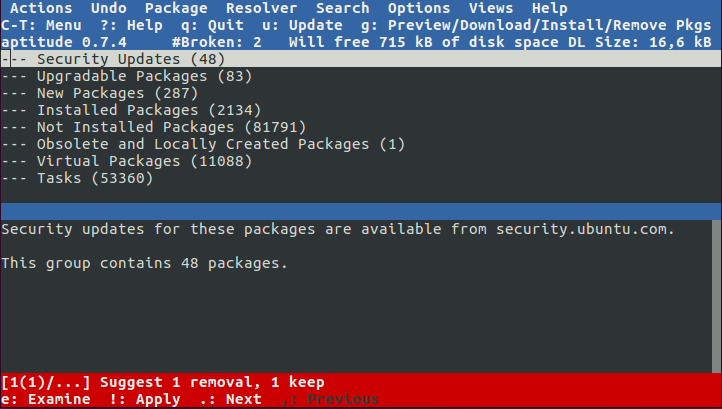
\includegraphics[width=0.7\textwidth]{Screenshot_aptitude.png}
	\caption{The command line visual interface for the $aptitude$ package manager.}
	\label{fig:aptitude_gui}
\end{figure}

\section{Development of Aptitude Module}\label{sec:aptitude_imp}
The implementation of the $aptitude$ module will be described here.
At first, the $aptitude$ class will be inherited from the abstract class $PackageManager$. 
This is presented in listing~\ref{lst:aptit_inher}. %\\
After that, the $aptitude$ class can be used as a regular package manager module, but it lacking functionality.
It is necessary to add the common code, like the constructor and the manager's name.
After these operations, the $aptitude$ module can be presented in listing~\ref{lst:aptit_common}. %\\
\begin{Listing} 
	\caption{The $aptitude$ inherited from the $PackageManager$ abstract class}
	\label{lst:aptit_inher}
\begin{lstlisting}
public final class PM_aptitude extends PackageManager {
	@Override
	public List<String> proceed(String filename, String source)
		throws FileNotFoundException, IOException, JAXBException {
		// TODO Auto-generated method stub
	}
}
\end{lstlisting}
\end{Listing} 
\begin{Listing} 
\caption{The $aptitude$ module with some common elements}
\label{lst:aptit_common}
\begin{lstlisting}
public final class PM_aptitude extends PackageManager {

	// name of the package manager
	static public final String Name = "aptitude";
	
	/**
	* Constructor
	*/
	public PM_aptitude(Language language, CSAR_handler ch) {
		this.language = language;
		this.ch = ch;
	}
	
	@Override
	public List<String> proceed(String filename, String source)
		throws FileNotFoundException, IOException, JAXBException {
		// TODO Auto-generated method stub
	}
}
\end{lstlisting}
\end{Listing} 
Since the package manager will read files from an input CSAR, the CSAR handler is stored by the constructor to the $ch$ variable for a further use.
In addition, a pointer to the language (to Bash in this case) is stored too, to be propagated later to the package handler.\\
Now consider the $proceed$ function.
A line-by-line file analyzer is needed.
It must modify the data and in the case of changes, the $isChanged$ variable should be set to $true$.
The $isChanged$ variable indicates that the file must be rewritten with a new content from the $newFile$ variable.
In the $output$ variable a set of packages from the package handler will be stored and returned back to the Bash module.
Described behavior is implemented in listing~\ref{lst:aptit_proceed}.\\
An $aptitude$ line parser will be implemented.
It must read a line from the $line$ variable and store it or it's modified version into the $newFile$ variable.
If the data was changed, then the $isChanged$ variable must be set to $true$.
Any $aptitude$ package installation calls should be detected, commented out and its arguments (package names) should be propagated one by one to the package handler's function $getPackage$. 
The result of the $getPackage$ function will be added to the $output$ variable.\\
During the parsing which is defined in the listing \ref{lst:aptit_parse}, the line is divided into words. 
Each found package name is transmitted to the packet handler as an argument of its public function $getPackage$.
In additional, this function must take the language and the source artifact's name as the arguments.
\begin{Listing} 
\caption{The aptitude $proceed$ function}
\label{lst:aptit_proceed}
\begin{lstlisting}
@Override
public void proceed(String filename, String source)
	throws FileNotFoundException, IOException, JAXBException {
	if (ch == null)
		throw new NullPointerException();
	List<String> output = new LinkedList<String>();
	System.out.println(Name + " proceed " + filename);
	BufferedReader br = new BufferedReader(new FileReader(filename));
	boolean isChanged = false;
	String line = null;
	String newFile = "";
	while ((line = br.readLine()) != null) {
		// TODO parsing will be done here
	}
	br.close();
	if (isChanged)
		Utils.createFile(filename,newFile);
	return output;
}	 
\end{lstlisting}
\end{Listing} 
\begin{Listing} 
\caption{The aptitude line parser}
\label{lst:aptit_parse}
\begin{lstlisting}
String[] words = line.replaceAll("[;&]", "").split("\\s+");
// skip spaces at the beginning of string
int i = 0;
if (words[i].equals(""))
	i = 1;
// looking for aptitude 
if (words.length >= 1 + i && words[i].equals("aptitude")) {
	// aptitude found
	if (words.length >= 3 + i && words[1 + i].equals("install")) {
		System.out.println("aptitude found:" + line);
		isChanged = true;
		for (int packet = 2 + i; packet < words.length; packet++) {
			System.out.println("package: " + words[packet]);
			output.addAll(ch.getPackage(language, words[packet], source));
		}
	}
	newFile += "#//References resolver//" + line + '\n';
} 
else
	newFile += line + '\n';
\end{lstlisting}
\end{Listing} 
%\subsection*{Integration Aptitude into the Bash Module}\label{sec:aptitude_int}
\\
Now the $aptitude$ module can be added to the Bash module.
The only thing to do is to add the $aptitude$ to the Bash's list of package manager modules (the list is stored in the \emph{packageManagers} variable).
This is done by the Bash's constructor with the command: \emph{"packageManagers.add(new PM\_aptitude(this, ch));"}. %\\
After these operation the new module is ready to identify and resolve external references which use the $aptitude$ package manager to install packages.
% !TeX spellcheck = en_US

\chapter{Check}\label{chap:check}
In this chapter, the developed framework will be tested.
The resulting CSAR will be added to \nameref{subs:wine} and displayed by the program.
\if 0 
%TODO
надо прописать какой именно архив использовался и какие в нём зависимости
потом установить как то хз как
\fi
\section{Check by Winery}
 \nameref{subs:wine} was installed to test the correctness of output CSAR. 
 This is an environment for development TOSCA systems and will be useful for checking results. \\
 The source CSAR is displayed on figure 
 %TODO
 This CSAR has a purely simple structure.
 THen the output CSAR was added to winery. 
 Due to significant increase in size, this can be a fairly lengthy procedure.
 There where 10 nodes in source CSAR, then after processing bz the framework, there are already more then 100 of nodes.
 During the addition, a CSAR's syntax is tested.
 In case of errors, messages will be displayed.
 Then Service Template will be displayed.
 Again, due to high number of nodes, preprocessing can take a long time. But at the time, the correctness of the links will be checked.
 If something was defined not properly, the nodes or links between them will not be displayed.
 After removing of external references and integrating python's dependency tree, the CSAR has acquired the following form (figure ).
 %TODO
 It's pretty beloved.
 To verify the TOSCA's structure some nodes was moved manually. 
 By checking several nodes with $apt$-$cache$ $depends$ command, the correctness of dependencies can be verified.
 By opening the content of the new nodes, it can be verified, that the are scripts and packages for installation.

\section{Check installation}
Also is is necessary to check whether it is possible to install new packages using the generated installation scripts.
First bash scripts will be tested, then ansible playbooks.
\subsection{Check bash scripts}
\if 0
Проверка сгенерированных баш скриптов это просто. 
Баш является стандартной средой командной строки в линукс, поэтому нужно просто выполнить эти скрипты и проверить корректность установки.
\fi
\subsection{Check ansible playbooks}

\if 0
\fi
% !TeX spellcheck = en_US

\chapter{Summary}\label{chap:zusfas}
%!!!Entwurf!!!\\
%The main points of this work will be presented and highlighted.\\  
External references can negatively affect the performance of cloud applications.
Unfortunately, many TOSCA applications access external sources to install various packages during a deployment.
If we have a high level of an information security or a limited access to the Internet, these external dependencies lead to a lot of problems which can be solved by encapsulation.
The purpose of this work was to develop a software for the elimination of such dependencies.\\
The software was developed in the Java language, which ensures its portability, ease of maintenance and extensibility.
To enable the ability to handle new types of external dependencies, the software was implemented in the form of a modular framework with separate modules for languages and package managers.
This allows a user to add their new handlers for package managers and languages easily.
In the first version, the framework handled only $Bash$ scripts  which use the $apt$-$get$ package manager.
To check the simplicity of the extensibility, the processing of $Bash$ scripts with the $aptitude$ package manager and  $Ansible$ playbooks with the $apt$ package manager was added.\\
The framework handles a CSAR as follows.
The structure of the CSAR is analyzed to determine the internal dependencies between artifacts and Node Templates.
Then each language module selects artifacts written in the language.
All such artifacts are transferred to the package managers of the language for processing.
They find external dependencies, remove them and pass the names of the required packages to the package handler.
It loads each package along with all its dependencies and sends information about them to the topology handler, which creates TOSCA nodes for these packages and defines TOSCA dependencies from the original nodes to the new ones.
Later, a runtime environment could analyze these dependencies and install the necessary packages.\\
In order to show the extensibility of the framework, the addition of the $aptitude$ package manager module into the $Bash$ module was described in the detail.
It  was shown how to create a module which can be added into the framework, how to implement its basic functions, pass data to the packet handler, and connect the module to $Bash$ language. \\
In the end, the results of the framework were validated.
The output SCARs were visualized and analyzed with the help of Winery.
Generated artifacts were tested and executed.\\
As a result, the framework was obtained that eliminates external dependencies in a CSAR.
It handles $Bash$ language with $aptitude$ and $apt$-$get$ package managers and $Ansible$ language with $apt$ package managers.
the Framework can be easily expanded to handle additional types of external references. 

\if 0
В этой главе будут приведены и обощены основные моменты данной работы.

Внешние зависимости могут негативно влиять на работу облачных приложениях.
К сожалению очень многие тоска приложения обращаются к внешним источникам для установки различных пакетов на этапе развёртки.
Если дело касается информационной безопастности или ограниченного доступа в интернет, то инкапсуляция приложения может решить множество проблем.
Целью данной работы было разработать софт для комплексного устранения таких зависимостей.

Софт разработан на языке ява, что обеспечивает его портируемость, простоту обслуживания и расширения.
Что бы дать возможность добавлять обработку новых типов внешних зависимостей, софт был выполнен в виде модульного фреймворка, с отдельными модулями для языков и менеджеров пакетов.
Это позволяет пользователю легко добавлять свои обработчики менеджеров пакетов и языков.
Изначально фреймворк обрабатывал только баш скрипты использующие менеджер пакетов апт-гет, но в ходе работы былы добавлены менеджер пакетов аптитуде для баш и Энсибл игровые книги с апт, для демонстрации простоту расширяемости фреймворка. 

Фреймворк обрабатывает ЦСАР следующим образом. 
Анализируется структура ЦСАР для определения внутренних зависимостей между артифактами и шаблонами ячеек.
Далее каждый модуль языков отфильтровывает артифакты, для написания которых использовался этот язык.
Все такие артифакты передаются на обработку модулям менеджеров пакетов этих языков. 
Находят внешние зависимости, устраняют их и передают имена необходимых пакетов обработчику пакетов.
Он загружает данный пакет вместе со всеми его зависимостями и предоставляет информацию о них обработчику топологии.
Обработчик топологии создаёт ячейки тоска данных пакетов и зависимости от изначальных ячеек к новым, так что бы в дальнейшем, среда выполнения могла проанализировать эти зависимости и установить необходимые пакеты самостоятельно.

Для того что бы показать расширяемость фреймворка процесс добавления моделя менеджера пакетов аптитудэ для баш был описан подробно. 
Было показано как создаётся модуль, который можно добавить во фреймворк, как имплементировать его основные функции, передавать данные обработчику пакетов и подключить модуль к языку баш.

в завершении были проверены результаты работы фреймворка.
Выходные ЦСАР были визуализированы и проанализированы с помощью вайнери.
Сгенерированные артефакты были протестированы и исполнены.

В результате был получен фреймворк, устраняющий внешние зависимости в ЦСАР.
Он обрабатывает такие то языки и может быть легко дополнен новыми модулями.

\fi
%
%% !TeX spellcheck = de_DE
%Die Angabe des schlauen Spruchs auf diesem Wege funtioniert nur,
%wenn keine Änderung des Kapitels mittels den in preambel/chapterheads.tex
%vorgeschlagenen Möglichkeiten durchgeführt wurde.
\setchapterpreamble[u]{%
\dictum[Albert Einstein]{Probleme kann man niemals mit derselben Denkweise lösen, durch die sie entstanden sind.}
}
\chapter{LaTeX-Tipps}
\label{chap:latextipps}

Pro Satz eine neue Zeile.
Das ist wichtig, um sauber versionieren zu können.
In LaTeX werden Absätze durch eine Leerzeile getrennt.

Folglich werden neue Abstäze insbesondere \emph{nicht} durch Doppelbackslashes erzeugt.
Der letzte Satz kam in einem neuen Absatz.

\section{File-Encoding und Unterstützung von Umlauten}
\label{sec:firstsectioninlatexhints}
Die Vorlage wurde 2010 auf UTF-8 umgestellt.
Alle neueren Editoren sollten damit keine Schwierigkeiten haben.

\section{Zitate}
Referenzen werden mittels \texttt{\textbackslash cite[key]} gesetzt.
Beispiel: \cite{WSPA} oder mit Autorenangabe: \citet{WSPA}.

Der folgende Satz demonstriert \begin{inparaenum}[1.]
\item die Großschreibung von Autorennamen am Satzanfang,
\item die richtige Zitation unter Verwendung von Autorennamen und der Referenz,
\item dass die Autorennamen ein Hyperlink auf das Literaturverzeichnis sind sowie
\item dass in dem Literaturverzeichnis der Namenspräfix \enquote{van der} von \enquote{Wil M.\,P.\ van der Aalst} steht.
\end{inparaenum}
\Citet{RVvdA2016} präsentieren eine Studie über die Effektivität von Workflow-Management-Systemen.

Der folgende Satz demonstriert, dass man mittels \texttt{label} in einem Bibliopgrahie"=Eintrag den Textteil des generierten Labels überschreiben kann, aber das Jahr und die Eindeutigkeit noch von biber generiert wird.
Die Apache ODE Engine \cite{ApacheODE} ist eine Workflow-Maschine, die BPEL-Prozesse zuverlässig ausführt.

Wörter am besten mittels \texttt{\textbackslash enquote\{...\}} \enquote{einschließen}, dann werden die richtigen Anführungszeichen verwendet.

Beim Erstellen der Bibtex-Datei wird empfohlen darauf zu achten, dass die DOI aufgeführt wird.

\section{Mathematische Formeln}
\label{sec:mf}
Mathematische Formeln kann man $so$ setzen. \texttt{symbols-a4.pdf} (zu finden auf \url{http://www.ctan.org/tex-archive/info/symbols/comprehensive/symbols-a4.pdf}) enthält eine Liste der unter LaTeX direkt verfügbaren Symbole.
Z.\,B.\ $\mathbb{N}$ für die Menge der natürlichen Zahlen.
Für eine vollständige Dokumentation für mathematischen Formelsatz sollte die Dokumentation zu \texttt{amsmath}, \url{ftp://ftp.ams.org/pub/tex/doc/amsmath/} gelesen werden.

Folgende Gleichung erhält keine Nummer, da \texttt{\textbackslash equation*} verwendet wurde.
\begin{equation*}
x = y
\end{equation*}

Die Gleichung~\ref{eq:test} erhält eine Nummer:
\begin{equation}
\label{eq:test}
x = y
\end{equation}

Eine ausführliche Anleitung zum Mathematikmodus von LaTeX findet sich in \url{http://www.ctan.org/tex-archive/help/Catalogue/entries/voss-mathmode.html}.

\section{Quellcode}
\Cref{lst:ListingANDlstlisting} zeigt, wie man Programmlistings einbindet.
Mittels \texttt{\textbackslash lstinputlisting} kann man den Inhalt direkt aus Dateien lesen.

%Listing-Umgebung wurde durch \newfloat{Listing} definiert
\begin{Listing}
\begin{lstlisting}
<listing name="second sample">
  <content>not interesting</content>
</listing>
\end{lstlisting}
\caption{lstlisting in einer Listings-Umgebung, damit das Listing durch Balken abgetrennt ist}
\label{lst:ListingANDlstlisting}
\end{Listing}

Quellcode im \lstinline|<listing />| ist auch möglich.

\section{Abbildungen}

Die \cref{fig:chor1} und \ref{fig:chor2} sind für das Verständnis dieses Dokuments wichtig.
Im Anhang zeigt \vref{fig:AnhangsChor} erneut die komplette Choreographie.

%Die Parameter in eckigen Klammern sind optionale Parameter - z.B. [htb!]
%htb! bedeutet: "Liebes LaTeX, bitte platziere diese Abbildung zuerst hier ("_h_ere"). Falls das nicht funktioniert, dann bitte oben auf der Seite ("_t_op"). Und falls das nicht geht, bitte unten auf der Seite ("_b_ottom"). Und bitte, bitte bevorzuge hier und oben, auch wenn's net so optimal aussieht ("!")
%Diese sollten nach Möglichkeit NICHT verwendet werden. LaTeX's Algorithmus für das Platzieren der Gleitumgebung ist schon sehr gut!
\begin{figure}
  \centering
  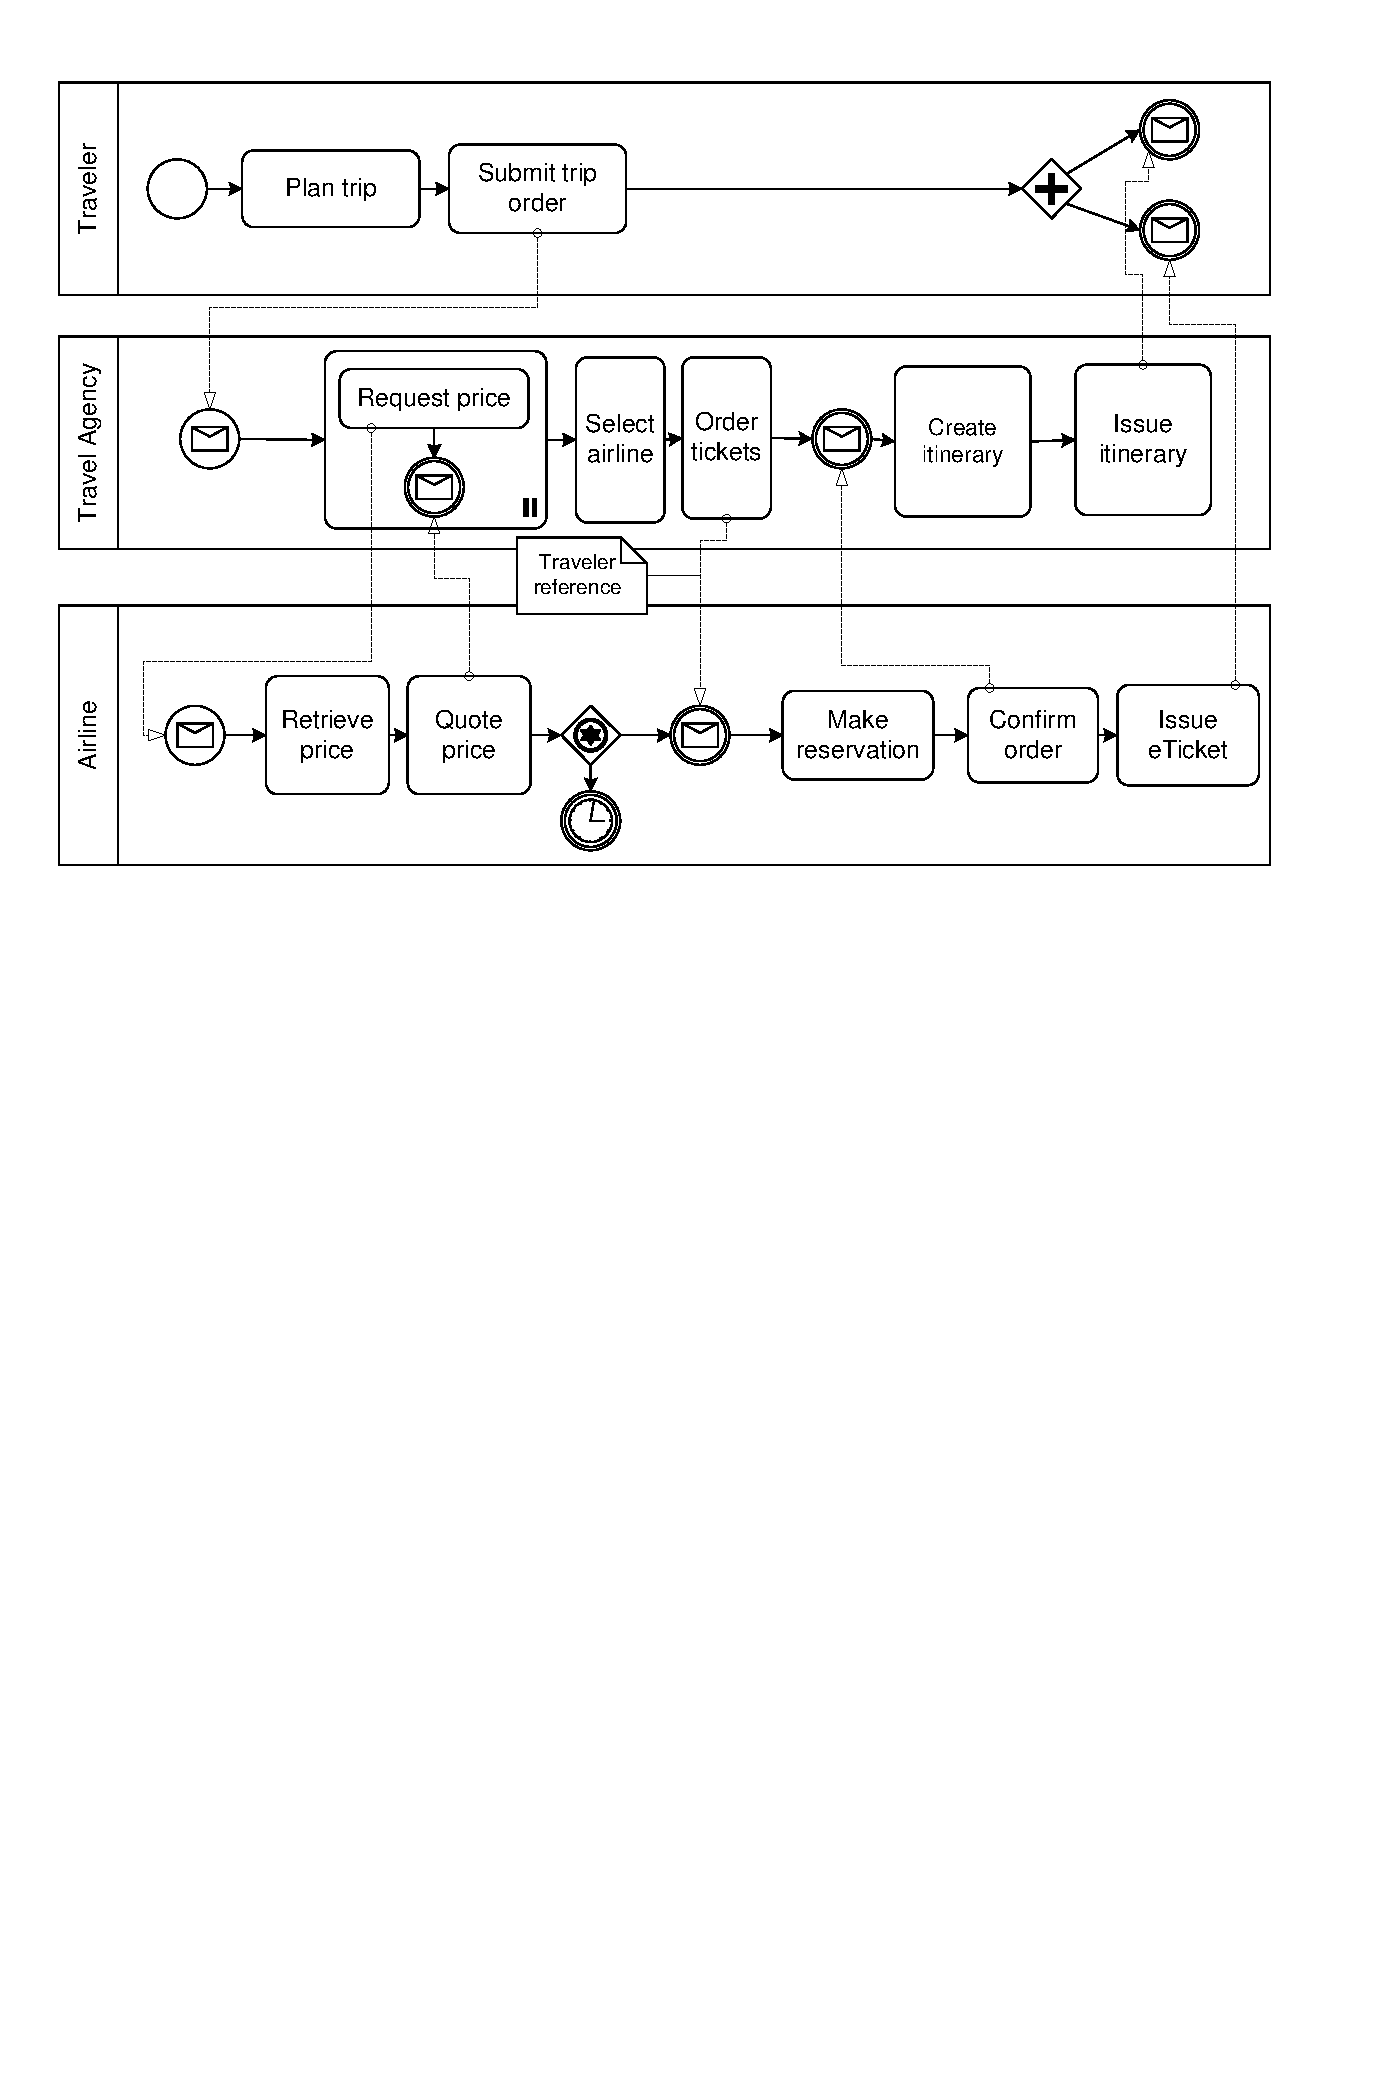
\includegraphics[width=\textwidth]{choreography.pdf}
  \caption{Beispiel-Choreographie}
  \label{fig:chor1}
\end{figure}

\begin{figure}
  \centering
  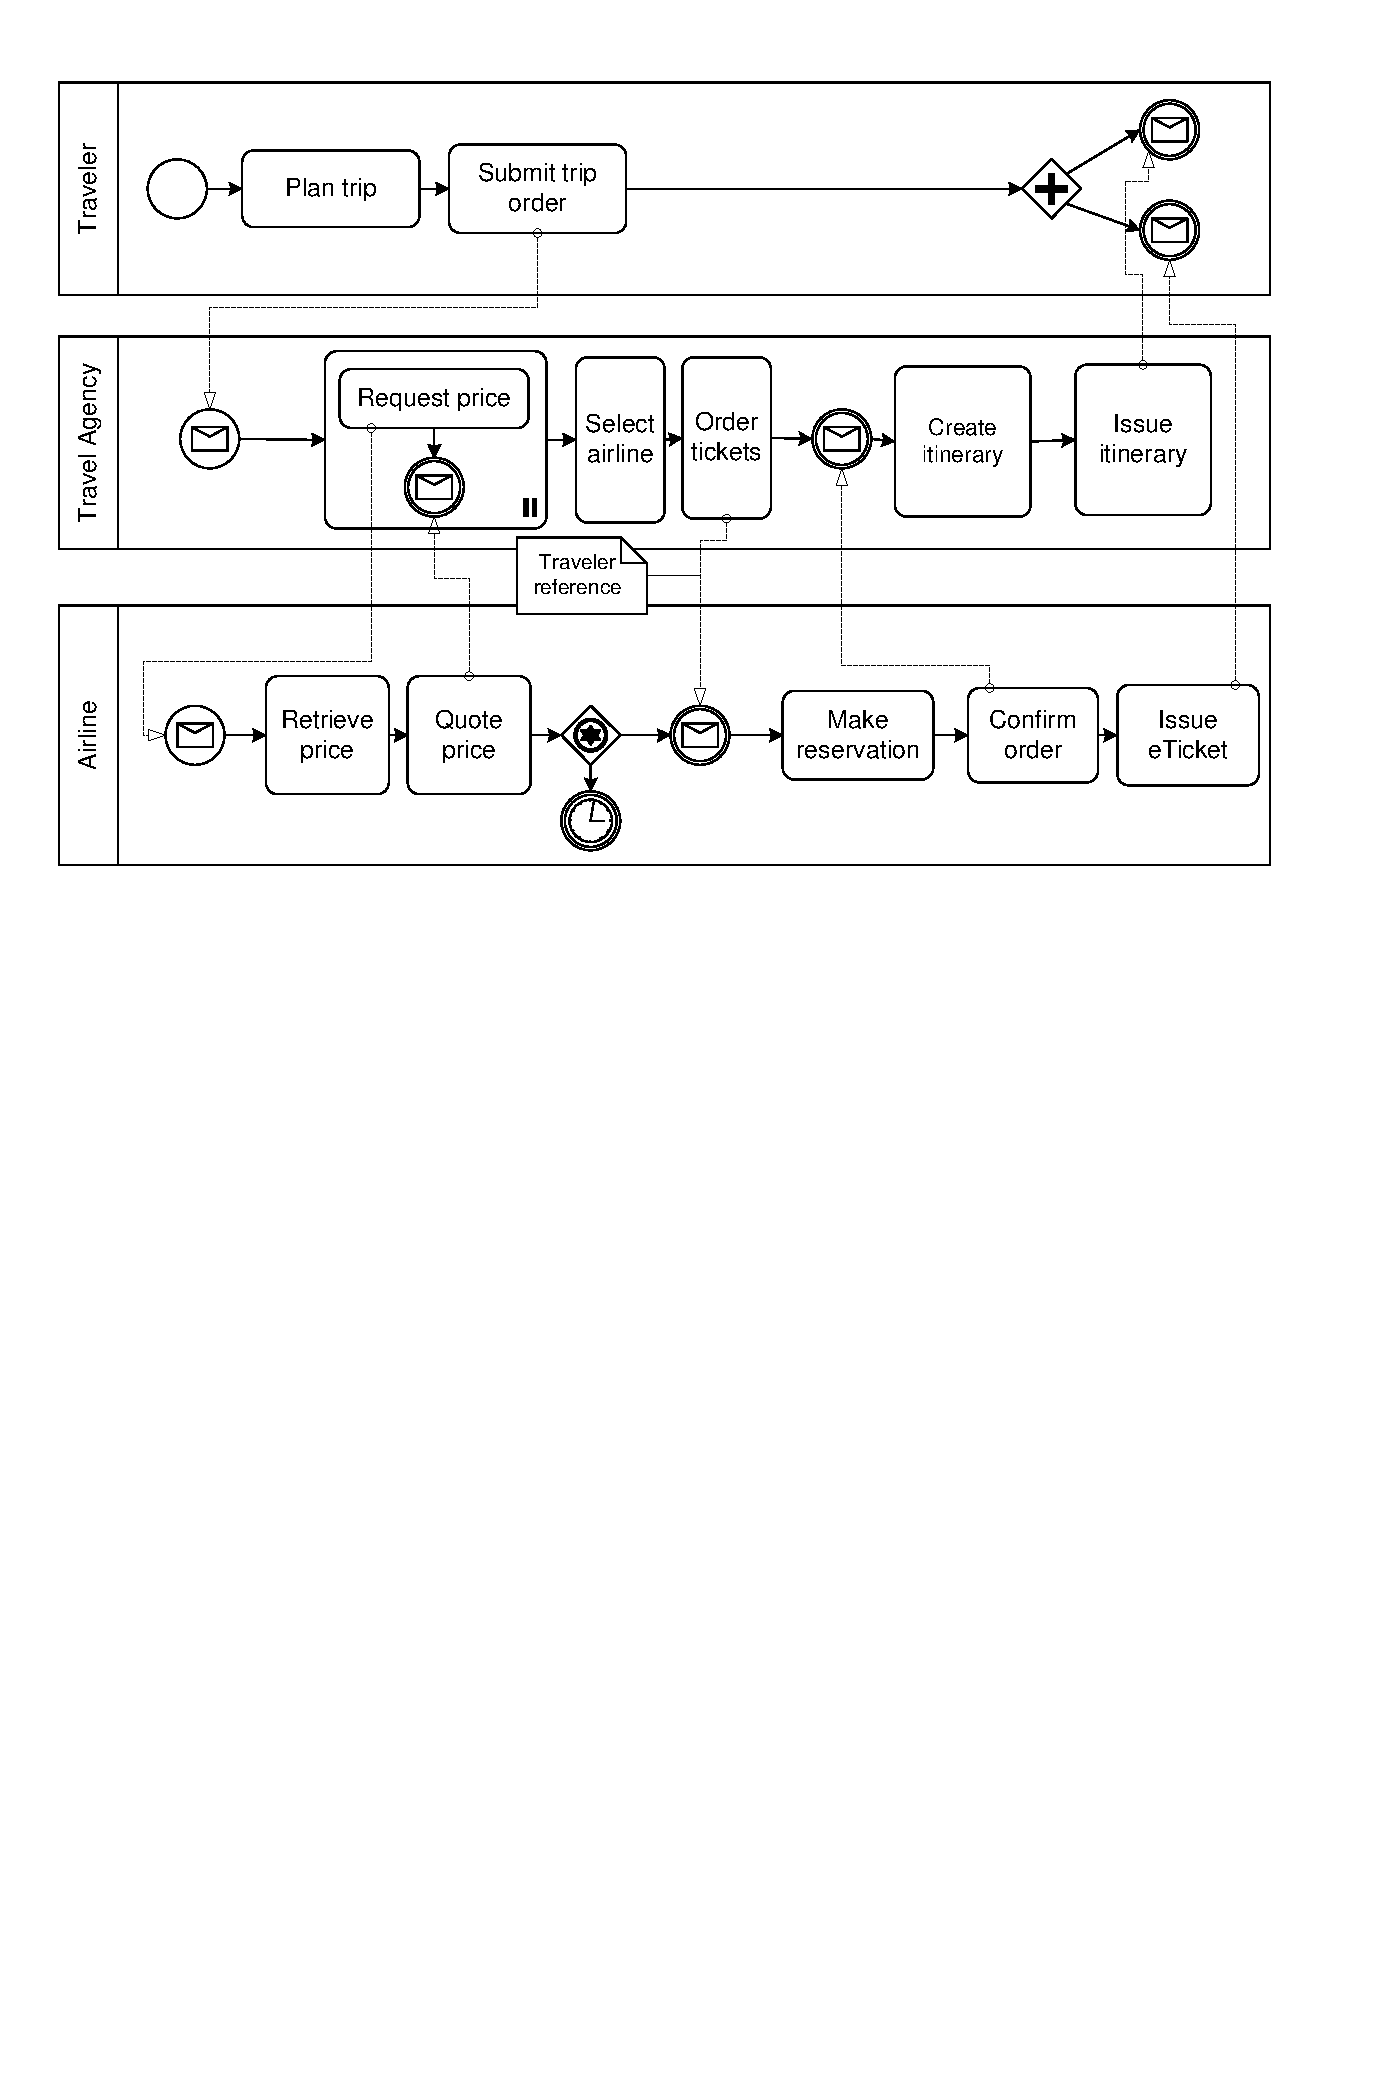
\includegraphics[width=.8\textwidth]{choreography.pdf}
  \caption[Beispiel-Choreographie]{Die Beispiel-Choreographie. Nun etwas kleiner, damit \texttt{\textbackslash textwidth} demonstriert wird. Und auch die Verwendung von alternativen Bildunterschriften für das Verzeichnis der Abbildungen. Letzteres ist allerdings nur Bedingt zu empfehlen, denn wer liest schon so viel Text unter einem Bild? Oder ist es einfach nur Stilsache?}
  \label{fig:chor2}
\end{figure}


\begin{figure}
  \centering
    \subfloat[]{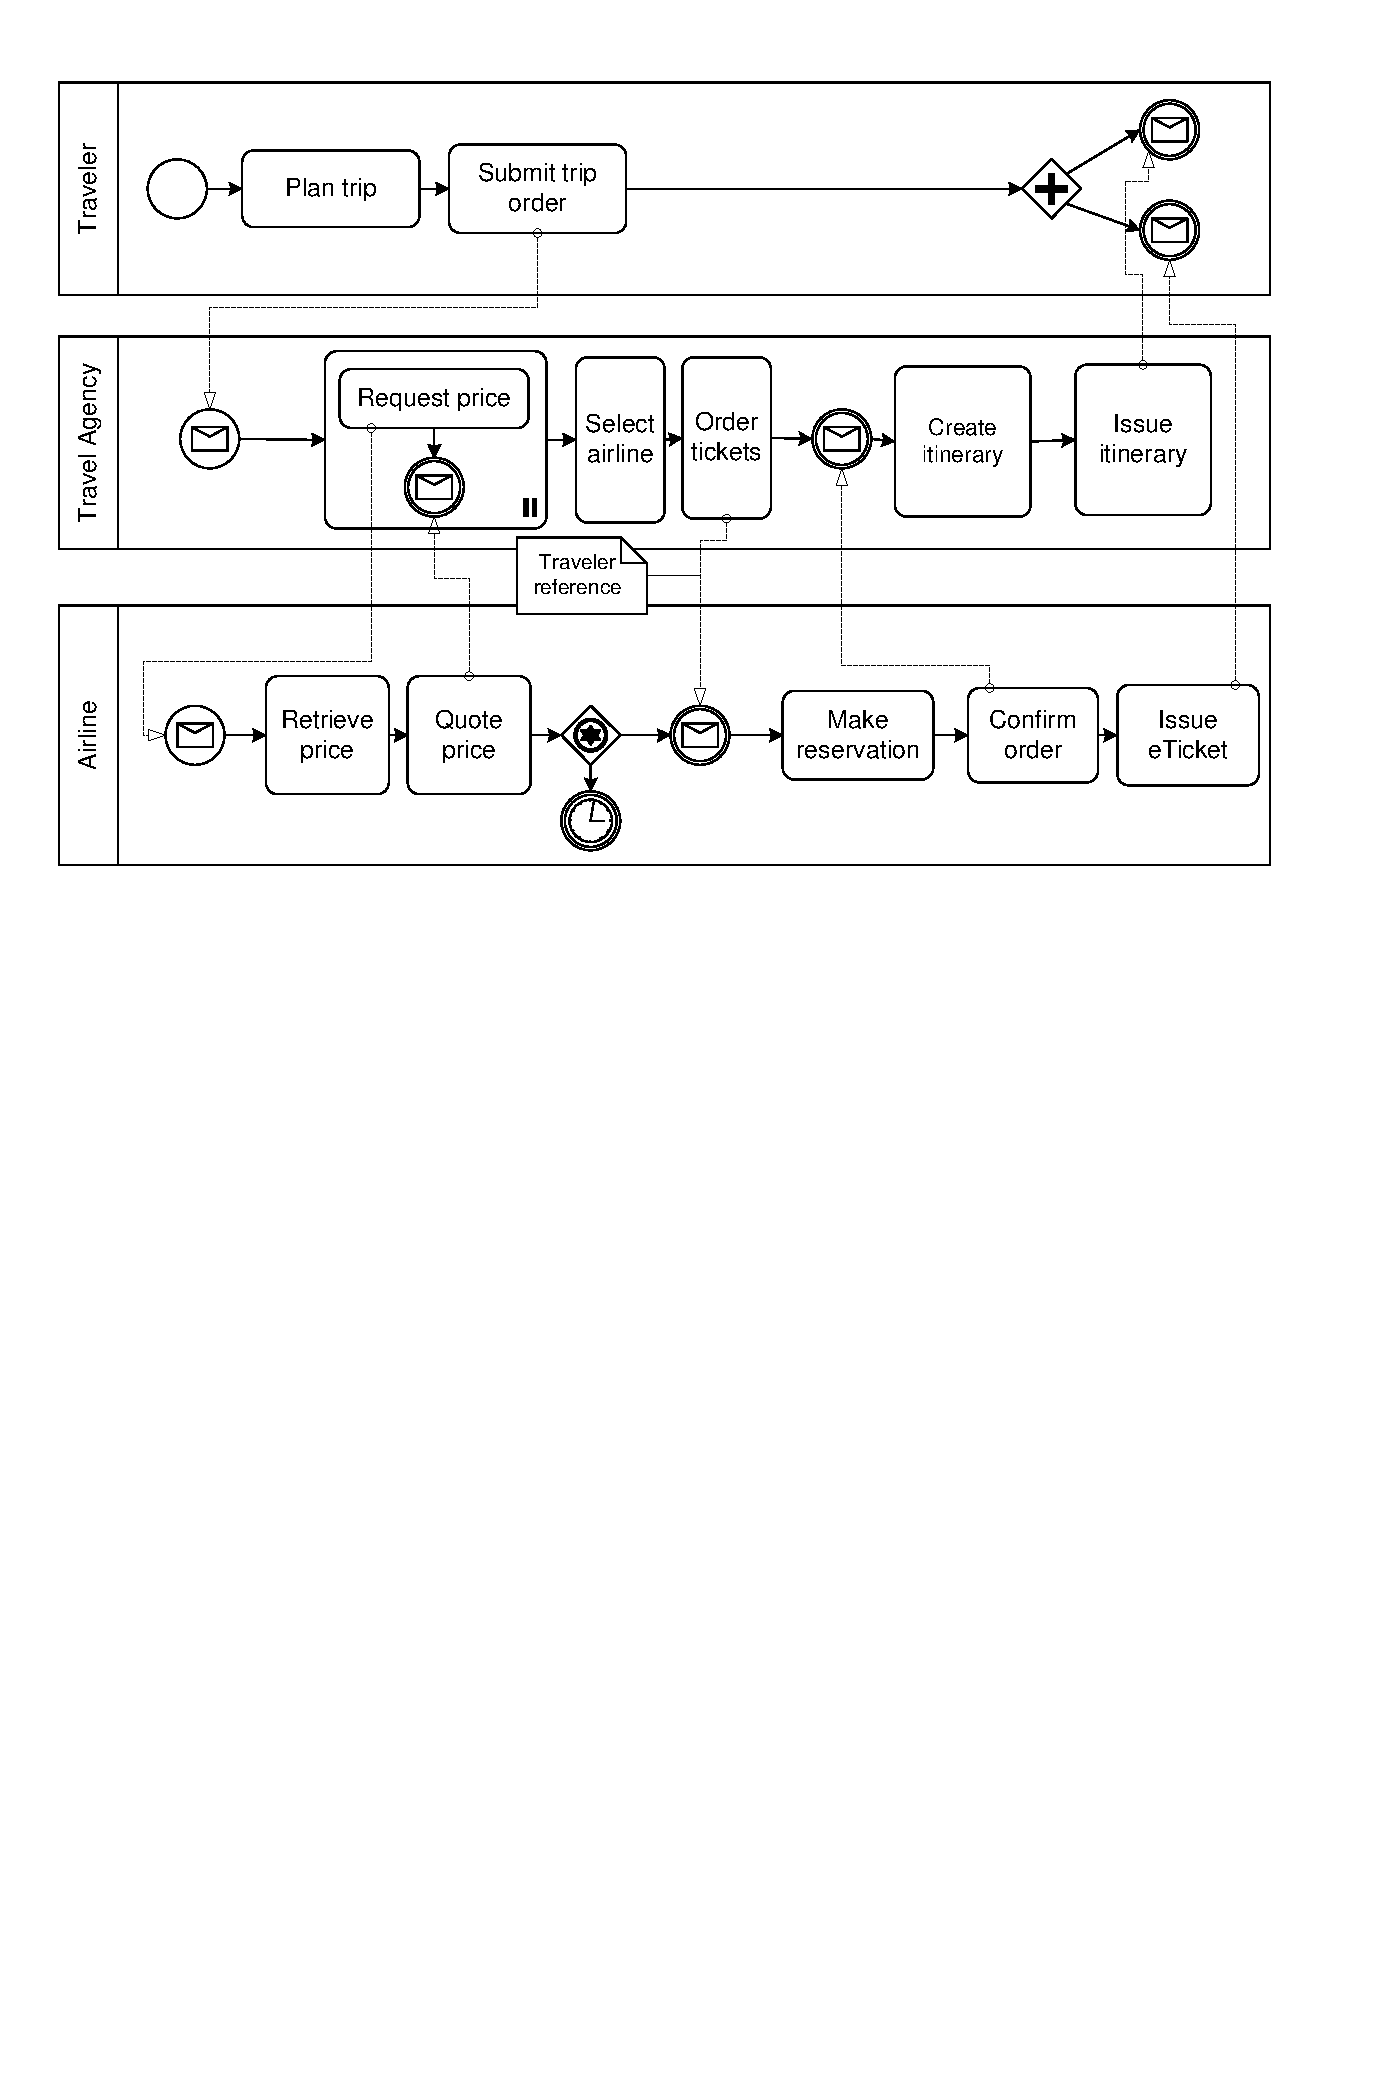
\includegraphics[width=0.3\textwidth]{choreography.pdf} \label{fig:subfigA}}
    \subfloat[]{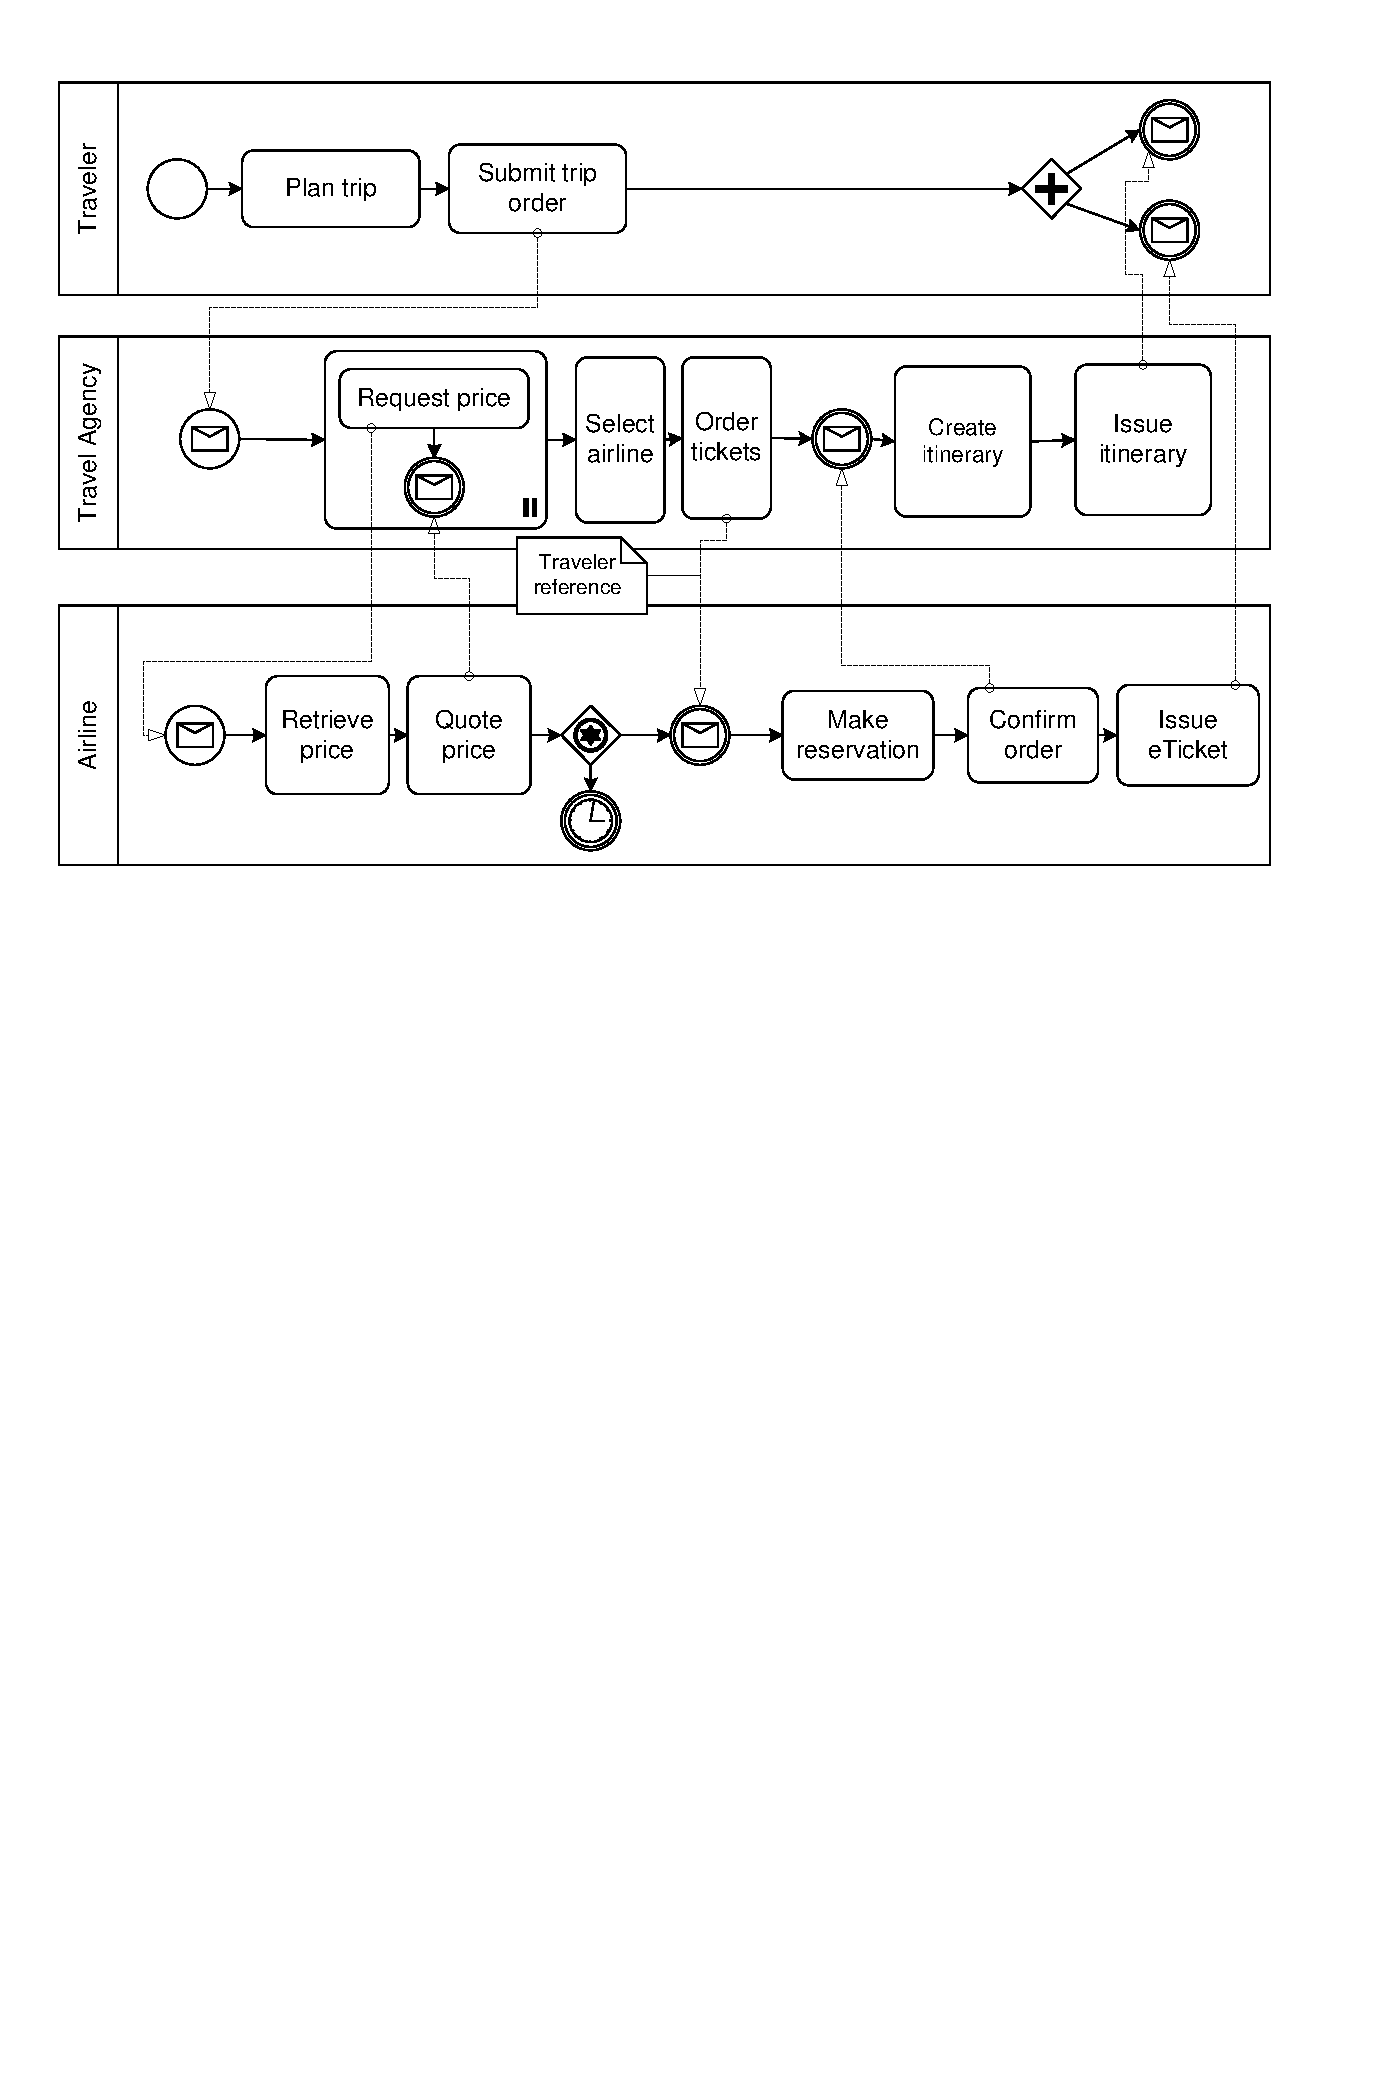
\includegraphics[width=0.3\textwidth]{choreography.pdf} \label{fig:subfigB}}
		\subfloat[Subcaption if needed]{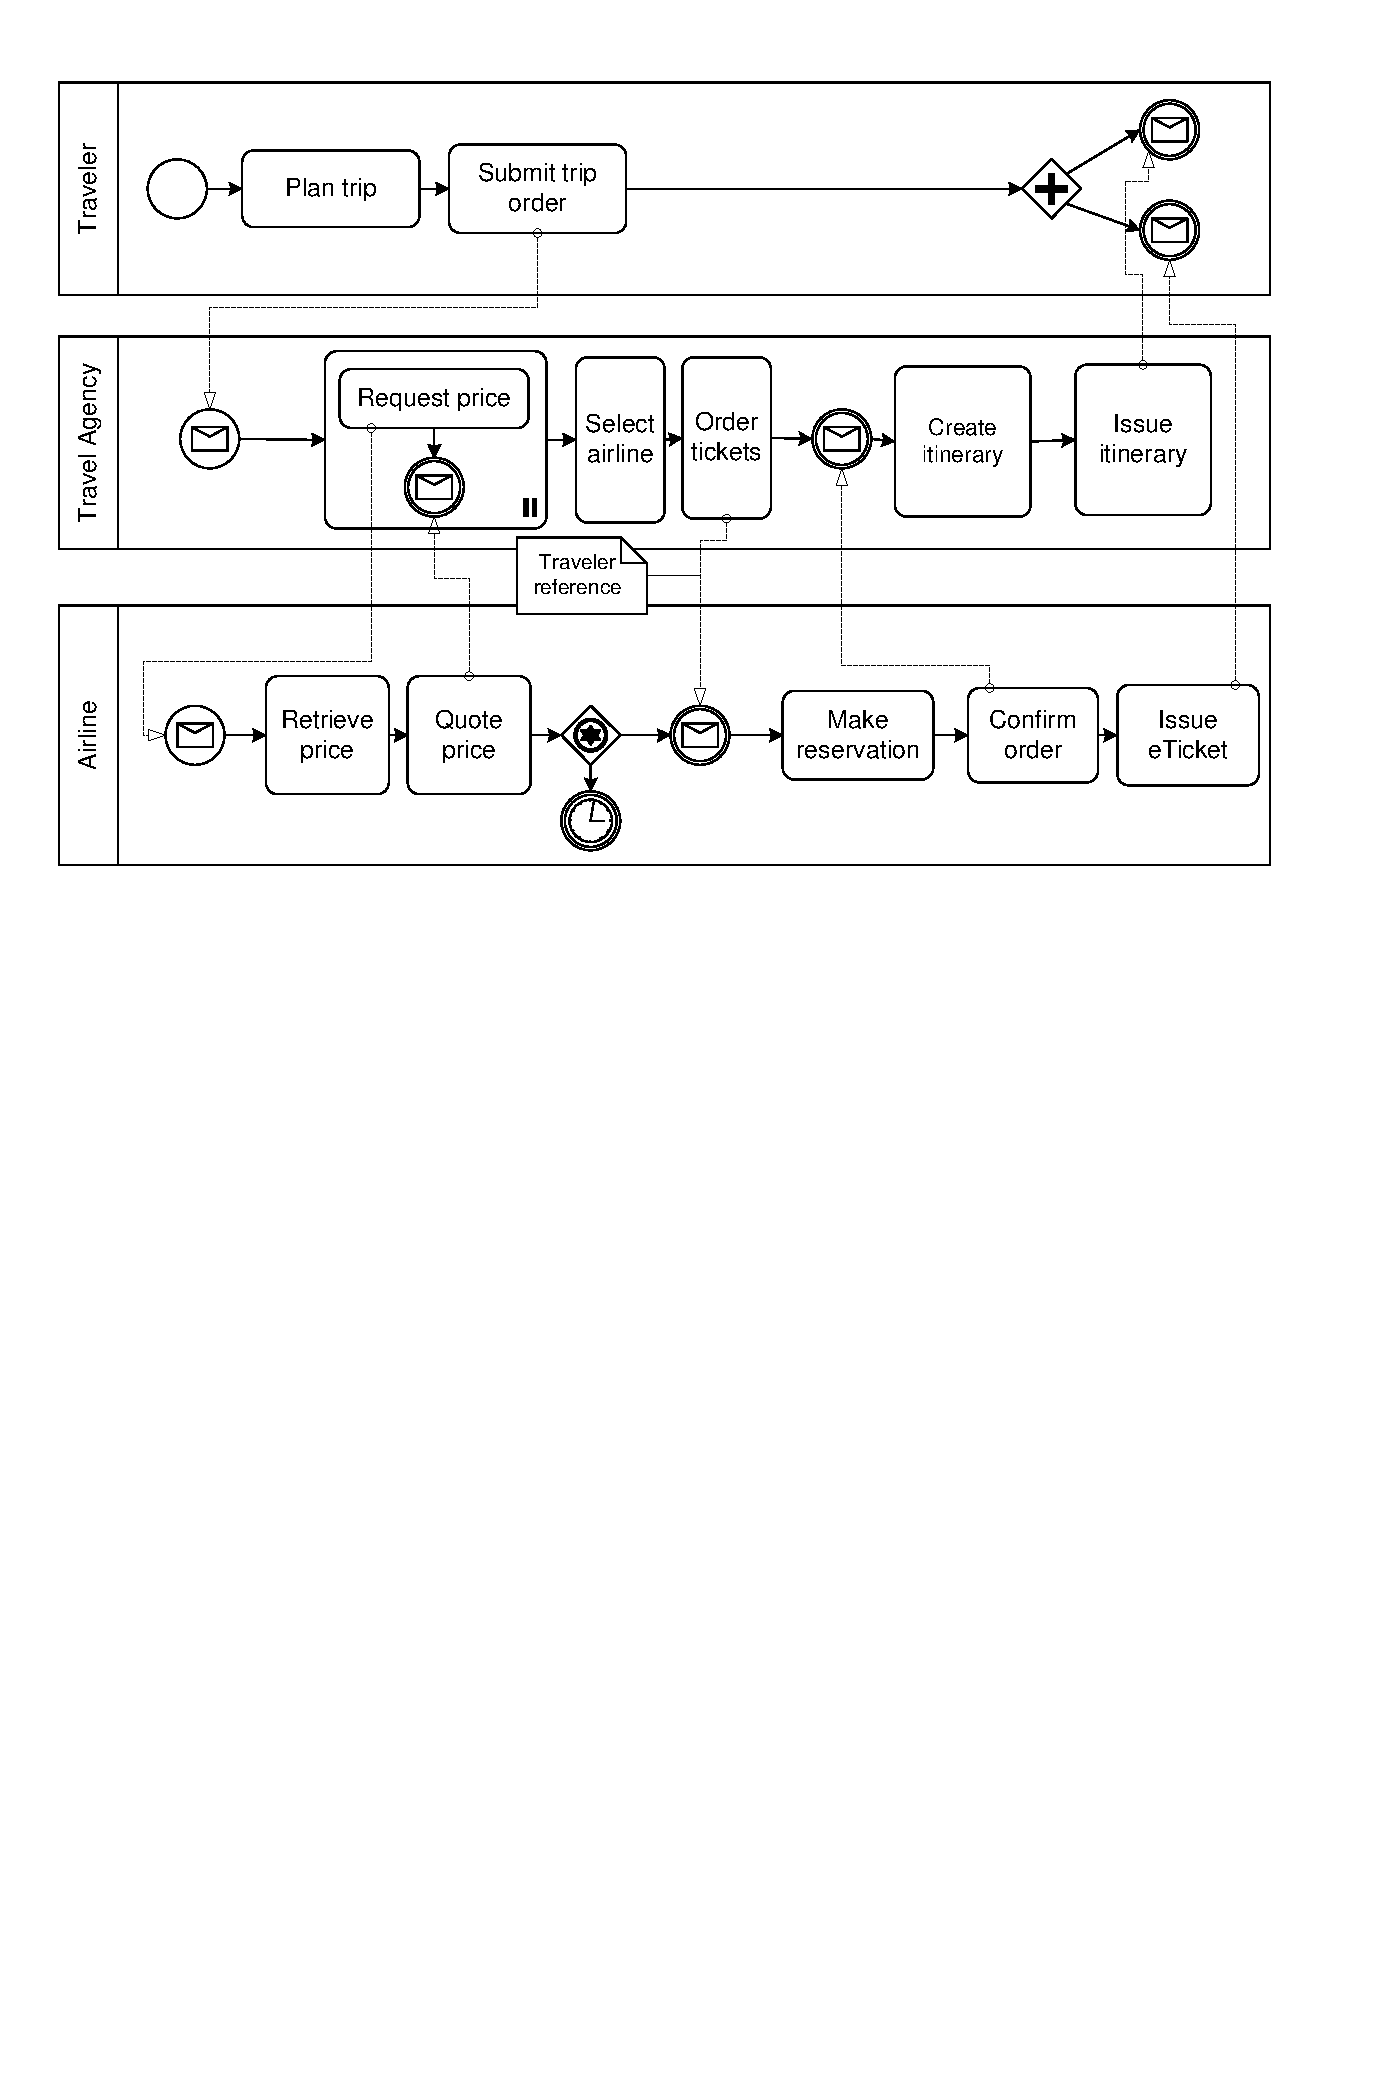
\includegraphics[width=0.3\textwidth]{choreography.pdf} \label{fig:subfigC}}
	\caption{Beispiel um 3 Abbildung nebeneinader zu stellen nur jedes einzeln referenzieren zu können. Abbildung~\ref{fig:subfigB}
 ist die mittlere Abbildung.}
\label{fig:subfig_example}
\end{figure}

Es ist möglich, SVGs direkt beim Kompilieren in PDF umzuwandeln.
Dies ist im Quellcode zu latex-tipps.tex beschrieben, allerdings auskommentiert.

\iffalse % <-- Das hier wegnehmen, falls inkscape im Pfad ist
Das SVG in \cref{fig:directSVG} ist direkt eingebunden, während der Text im SVG in \cref{fig:latexSVG} mittels pdflatex gesetzt ist.
Falls man die Graphiken sehen möchte, muss inkscape im PATH sein und im Tex-Quelltext \texttt{\textbackslash{}iffalse} und \texttt{\textbackslash{}iftrue} auskommentiert sein.

\begin{figure}
\centering

\includegraphics{svgexample.svg}
\caption{SVG direkt eingebunden}
\label{fig:directSVG}
\end{figure}

\begin{figure}
\centering
\def\svgwidth{.4\textwidth}
\includesvg{svgexample}
\caption{Text im SVG mittels \LaTeX{} gesetzt}
\label{fig:latexSVG}
\end{figure}
\fi % <-- Das hier wegnehmen, falls inkscape im Pfad ist

\section{Tabellen}

\cref{tab:Ergebnisse} zeigt Ergebnisse und die \cref{tab:Ergebnisse} zeigt wie numerische Daten in einer Tabelle representiert werden können.
\begin{table}
  \centering
  \begin{tabular}{ccc}
  \toprule
  \multicolumn{2}{c}{\textbf{zusammengefasst}} & \textbf{Titel} \\ \midrule
  Tabelle & wie & in \\
  \url{tabsatz.pdf}& empfohlen & gesetzt\\

  \multirow{2}{*}{Beispiel} & \multicolumn{2}{c}{ein schönes Beispiel}\\
   & \multicolumn{2}{c}{für die Verwendung von \enquote{multirow}}\\
  \bottomrule
  \end{tabular}
  \caption[Beispieltabelle]{Beispieltabelle -- siehe \url{http://www.ctan.org/tex-archive/info/german/tabsatz/}}
  \label{tab:Ergebnisse}
\end{table}

\begin{table}
	\centering
	\begin{tabular}{l *{8}{d{3.2}}}
		\toprule
						
			   & \multicolumn{2}{c}{\textbf{Parameter 1}} & \multicolumn{2}{c}{\textbf{Parameter 2}} & \multicolumn{2}{c}{\textbf{Parameter 3}} & \multicolumn{2}{c}{\textbf{Parameter 4}} \\
			\cmidrule(r){2-3}\cmidrule(lr){4-5}\cmidrule(lr){6-7}\cmidrule(l){8-9}
			
			\textbf{Bedingungen} & \multicolumn{1}{c}{\textbf{M}} & \multicolumn{1}{c}{\textbf{SD}} & \multicolumn{1}{c}{\textbf{M}} & \multicolumn{1}{c}{\textbf{SD}} & \multicolumn{1}{c}{\textbf{M}} & \multicolumn{1}{c}{\textbf{SD}} & \multicolumn{1}{c}{\textbf{M}} & \multicolumn{1}{c}{\textbf{SD}}\\
			\midrule
			
			W & 1.1 & 5.55 & 6.66 & .01 &  &  &  & \\
			X & 22.22 & 0.0 & 77.5 & .1 &  &  &  & \\
			Y & 333.3 & .1 & 11.11 & .05 &  &  &  & \\
			Z & 4444.44 & 77.77 & 14.06 & .3 &  &  &  & \\
		\bottomrule 
	\end{tabular}
	
	\caption{Beispieltabelle f\"{u}r 4 Bedingungen (W-Z) mit jeweils 4 Parameters mit (M und SD). Hinweiß: immer die selbe anzahl an Nachkommastellen angeben.}
	\label{tab:Werte}
\end{table}

\section{Pseudocode}
\Cref{alg:sample} zeigt einen Beispielalgorithmus.
\begin{Algorithmus} %Die Umgebung nur benutzen, wenn man den Algorithmus ähnlich wie Graphiken von TeX platzieren lassen möchte
\caption{Sample algorithm}
\label{alg:sample}
\begin{algorithmic}
\Procedure{Sample}{$a$,$v_e$}
\State $\mathsf{parentHandled} \gets (a = \mathsf{process}) \lor \mathsf{visited}(a'), (a',c,a) \in \mathsf{HR}$
\State \Comment $(a',c'a) \in \mathsf{HR}$ denotes that $a'$ is the parent of $a$
\If{$\mathsf{parentHandled}\,\land(\mathcal{L}_\mathit{in}(a)=\emptyset\,\lor\,\forall l \in \mathcal{L}_\mathit{in}(a): \mathsf{visited}(l))$}
\State $\mathsf{visited}(a) \gets \text{true}$
\State $\mathsf{writes}_\circ(a,v_e) \gets
\begin{cases}
\mathsf{joinLinks}(a,v_e) & \abs{\mathcal{L}_\mathit{in}(a)} > 0\\
\mathsf{writes}_\circ(p,v_e)
& \exists p: (p,c,a) \in \mathsf{HR}\\
(\emptyset, \emptyset, \emptyset, false) & \text{otherwise}
\end{cases}
$
\If{$a\in\mathcal{A}_\mathit{basic}$}
  \State \Call{HandleBasicActivity}{$a$,$v_e$}
\ElsIf{$a\in\mathcal{A}_\mathit{flow}$}
  \State \Call{HandleFlow}{$a$,$v_e$}
\ElsIf{$a = \mathsf{process}$} \Comment Directly handle the contained activity
  \State \Call{HandleActivity}{$a'$,$v_e$}, $(a,\bot,a') \in \mathsf{HR}$
  \State $\mathsf{writes}_\bullet(a) \gets \mathsf{writes}_\bullet(a')$
\EndIf
\ForAll{$l \in \mathcal{L}_\mathit{out}(a)$}
  \State \Call{HandleLink}{$l$,$v_e$}
\EndFor
\EndIf
\EndProcedure
\end{algorithmic}
\end{Algorithmus}

\clearpage
Und wer einen Algorithmus schreiben möchte, der über mehrere Seiten geht, der kann das nur mit folgendem \textbf{üblen} Hack tun:

{
\begin{minipage}{\textwidth}
\hrule height .8pt width\textwidth
\vskip.3em%\vskip\abovecaptionskip\relax
\stepcounter{Algorithmus}
\addcontentsline{alg}{Algorithmus}{\protect\numberline{\theAlgorithmus}{\ignorespaces Description \relax}}
\noindent\textbf{Algorithmus \theAlgorithmus} Description
%\stepcounter{algorithm}
%\addcontentsline{alg}{Algorithmus}{\thealgorithm{}\hskip0em Description}
%\textbf{Algorithmus \thealgorithm} Description
\vskip.3em%\vskip\belowcaptionskip\relax
\hrule height .5pt width\textwidth
\end{minipage}
%without the following line, the text is nerer at the rule
\vskip-.3em
%
code goes here\\
test2\\
%
\vskip-.7em
\hrule height .5pt width\textwidth
}


\section{Abkürzungen}

Beim ersten Durchlauf betrug die \gls{fr} 5.
Beim zweiten Durchlauf war die \gls{fr} 3.~Die Pluralform sieht man hier:\ \glspl{er}.
Um zu demonstrieren, wie das Abkürzungsverzeichnis bei längeren Beschreibungstexten aussieht, muss hier noch \glspl{rdbms} erwähnt werden.

Mit \verb+\gls{...}+ können Abkürzungen eingebaut werden, beim ersten Aufrufen wird die lange Form eingesetzt.
Beim wiederholten Verwenden von \verb+\gls{...}+ wird automatisch die kurz Form angezeigt.
Außerdem wird die Abkürzung automatisch in die Abkürzungsliste eingefügt.
Mit \verb+\glspl{...}+ wird die Pluralform verwendet.
Möchte man, dass bei der ersten Verwendung direkt die Kurzform erscheint, so kann man mit \verb+\glsunset{...}+ eine Abkürzung als bereits verwendet markieren.
Das Gegenteil erreicht man mit \verb+\glsreset{...}+.

Definiert werden Abkürzungen in der Datei \textit{content\\ausarbeitung.tex} mithilfe von \verb+\newacronym{...}{...}{...}+.

Mehr Infos unter: \url{http://tug.ctan.org/macros/latex/contrib/glossaries/glossariesbegin.pdf}

\section{Verweise}
Für weit entfernte Abschnitte ist \enquote{varioref} zu empfehlen:
\enquote{Siehe \vref{sec:mf}}.
Das Kommando \texttt{\textbackslash{}vref} funktioniert ähnlich wie \texttt{\textbackslash{}cref} mit dem Unterschied, dass zusätzlich ein Verweis auf die Seite hinzugefügt wird.
\texttt{vref}: \enquote{\vref{sec:firstsectioninlatexhints}}, \texttt{cref}: \enquote{\cref{sec:firstsectioninlatexhints}}, \texttt{ref}: \enquote{\ref{sec:firstsectioninlatexhints}}.

Falls \enquote{varioref} Schwierigkeiten macht, dann kann man stattdessen \enquote{cref} verwenden.
Dies erzeugt auch das Wort \enquote{Abschnitt} automatisch: \cref{sec:mf}.
Das geht auch für Abbildungen usw.
Im Englischen bitte \verb1\Cref{...}1 (mit großem \enquote{C} am Anfang) verwenden.


%Mit MiKTeX Installation ab dem 2012-01-16 nicht mehr nötig
%Falls ein Abschnitt länger als eine Seite wird und man mittels \texttt{\textbackslash{}vref} auf eine konkrete Stelle in der Section
%verweisen möchte, dann sollte man \texttt{\textbackslash{}phantomsection} verwenden und dann wird
%auch bei \texttt{vref} die richtige Seite angeben.

%%The link location will be placed on the line below.
%%Tipp von http://en.wikibooks.org/wiki/LaTeX/Labels_and_Cross-referencing#The_hyperref_package_and_.5Cphantomsection
%\phantomsection
%\label{alabel}
%Das Beispiel für \texttt{\textbackslash{}phantomsection} bitte im \LaTeX{}-Quellcode anschauen.

%Hier das Beispiel: Siehe Abschnitt \vref{hack1} und Abschnitt \vref{hack2}.

\section{Definitionen}
\begin{definition}[Title]
\label{def:def1}
Definition Text
\end{definition}

\Cref{def:def1} zeigt \ldots

\section{Fußnoten}
Fußnoten können mit dem Befehl \verb+\footnote{...}+ gesetzt werden\footnote{\label{fussnote}Diese Fußnote ist ein Beispiel.}. Mehrfache Verwendung von Fußnoten ist möglich indem man zu erst ein Label in der Fußnote setzt \verb+\footnote{\label{...}...}+ und anschließend mittels \verb+\cref{...}+ die Fußnote erneut verwendet\cref{fussnote}.

\section{Verschiedenes}
\label{sec:diff}
\ifdeutsch
Ziffern (123\,654\,789) werden schön gesetzt.
Entweder in einer Linie oder als Minuskel-Ziffern.
Letzteres erreicht man durch den Parameter \texttt{osf} bei dem Paket \texttt{libertine} bzw.\ \texttt{mathpazo} in \texttt{fonts.tex}.
\fi

\textsc{Kapitälchen} werden schön gesperrt...

\begin{compactenum}[I.]
\item Man kann auch die Nummerierung dank paralist kompakt halten
\item und auf eine andere Nummerierung umstellen
\end{compactenum}

\section{Weitere Illustrationen}
\Cref{fig:AnhangsChor,fig:AnhangsChor2} zeigen zwei Choreographien, die den Sachverhalt weiter erläutern sollen.
Die zweite Abbildung ist um 90 Grad gedreht, um das Paket \texttt{pdflscape} zu demonstrieren.

\begin{figure}
  \centering
  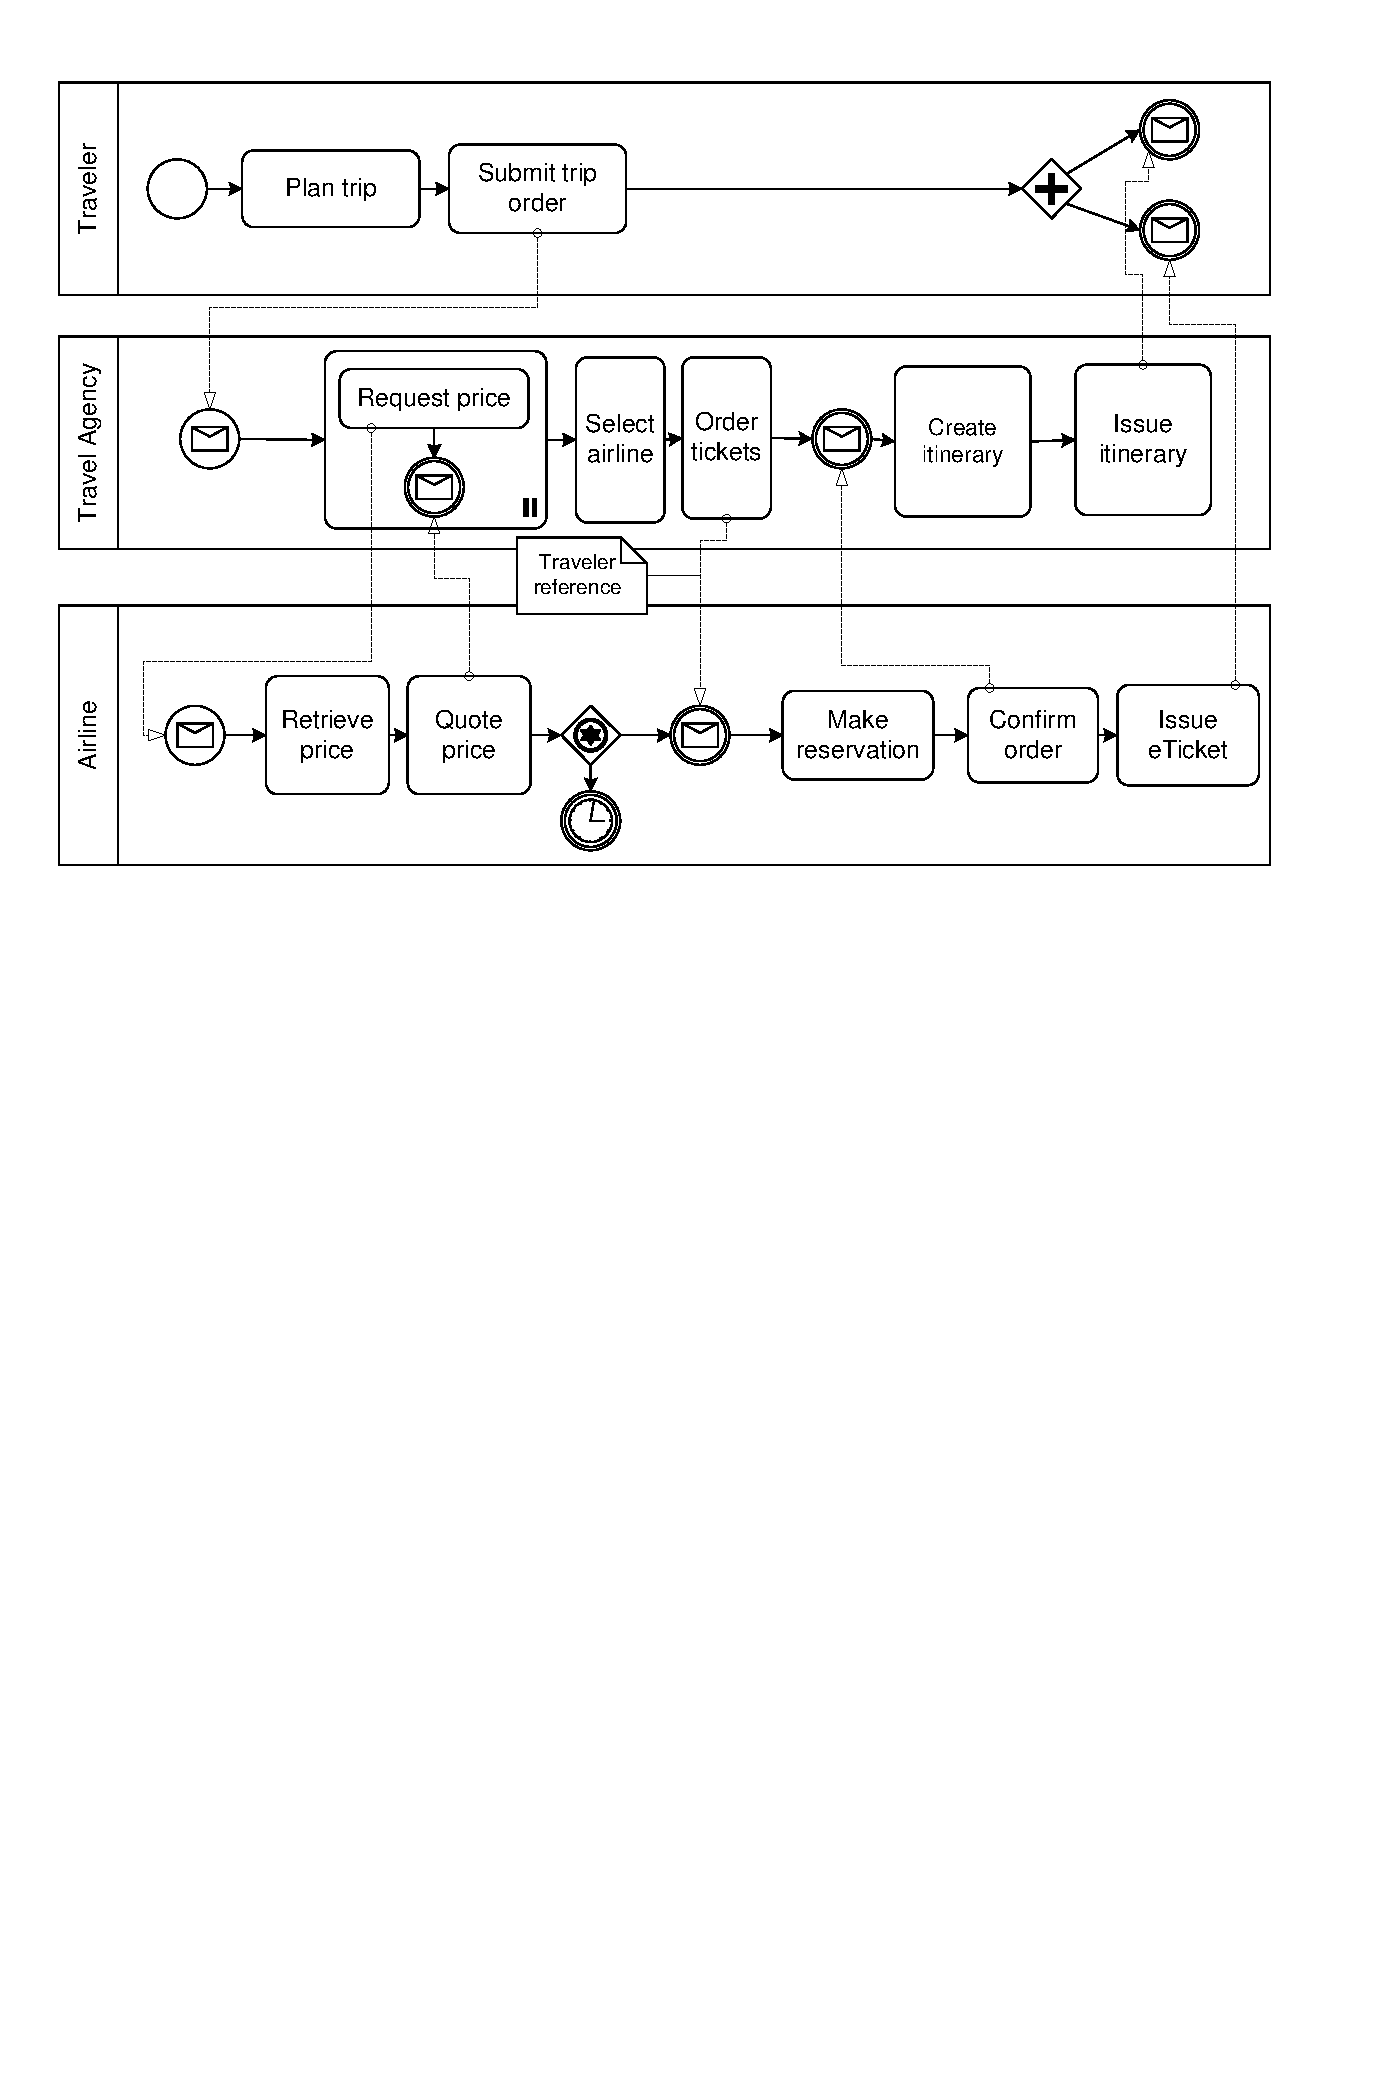
\includegraphics[width=\textwidth]{choreography.pdf}
  \caption{Beispiel-Choreographie I}
  \label{fig:AnhangsChor}
\end{figure}

\begin{landscape}
  \begin{figure}
    \centering
    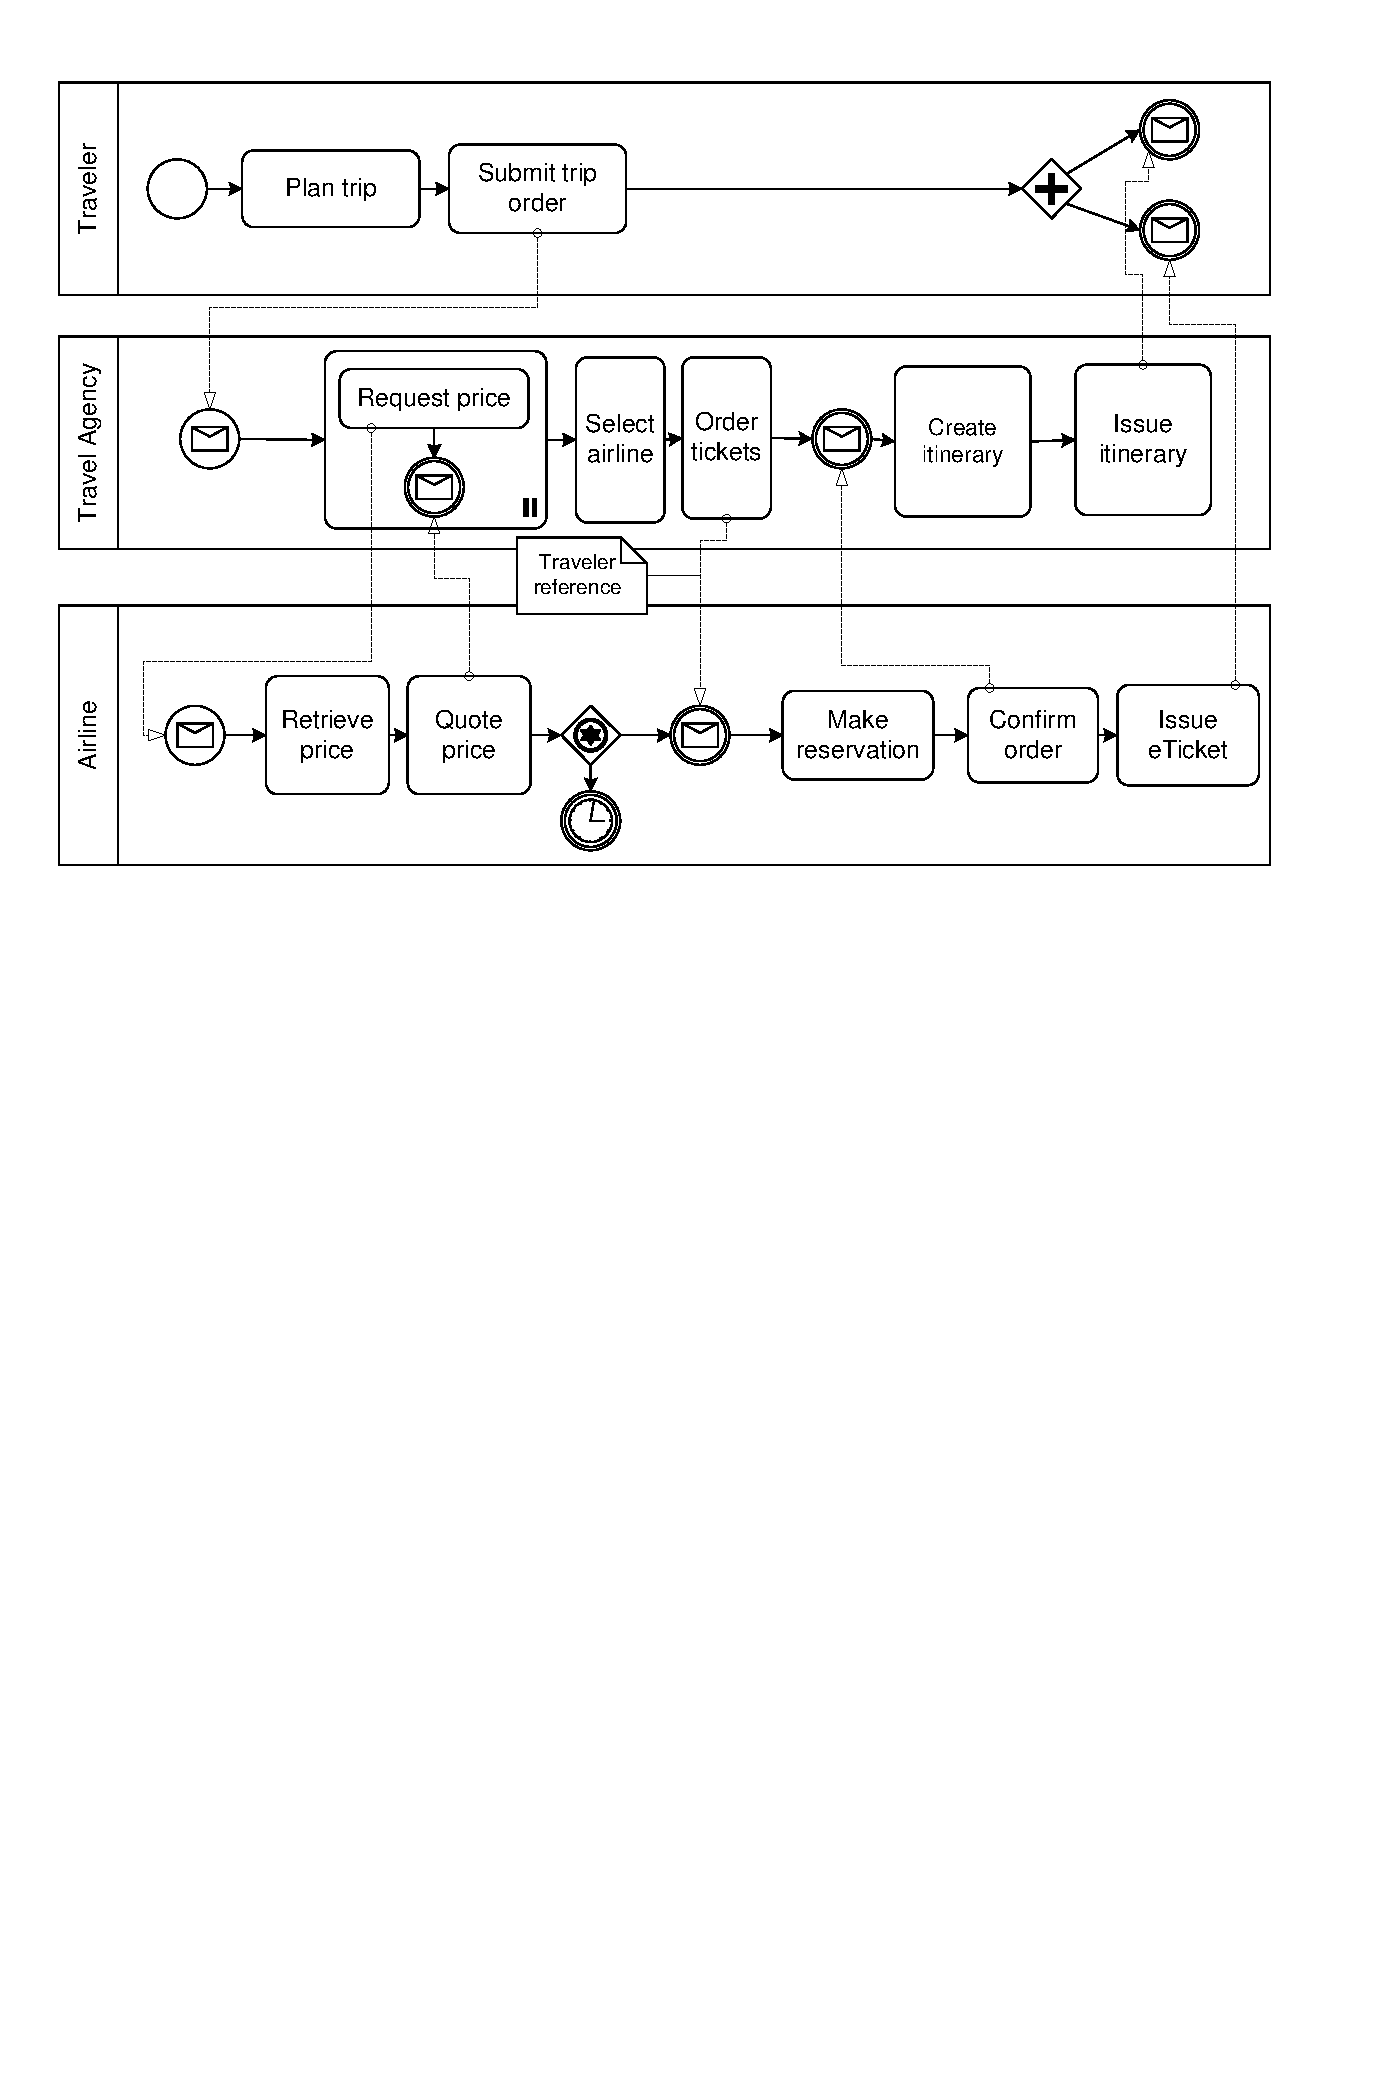
\includegraphics[width=\textwidth]{choreography.pdf}
    \caption{Beispiel-Choreographie II}
    \label{fig:AnhangsChor2}
  \end{figure}
\end{landscape}


\iffalse

\clearpage

FIXME - This does not work with MiKTeX as of 2016-12-30

TODO- demonstrate rotating package

%hint by http://tex.stackexchange.com/a/3265/9075
%other option is to use changepage according to http://tex.stackexchange.com/a/2639/9075. This, however, has issues with landscape
\thispagestyle{empty}

\savegeometry{koma}

%If you only have height problems, this is not needed at all
\addtolength{\textwidth}{2cm}
\addtolength{\evensidemargin}{-1cm}

\begin{landscape}
  %sidewaysfigure
  \begin{figure}
    \centering
    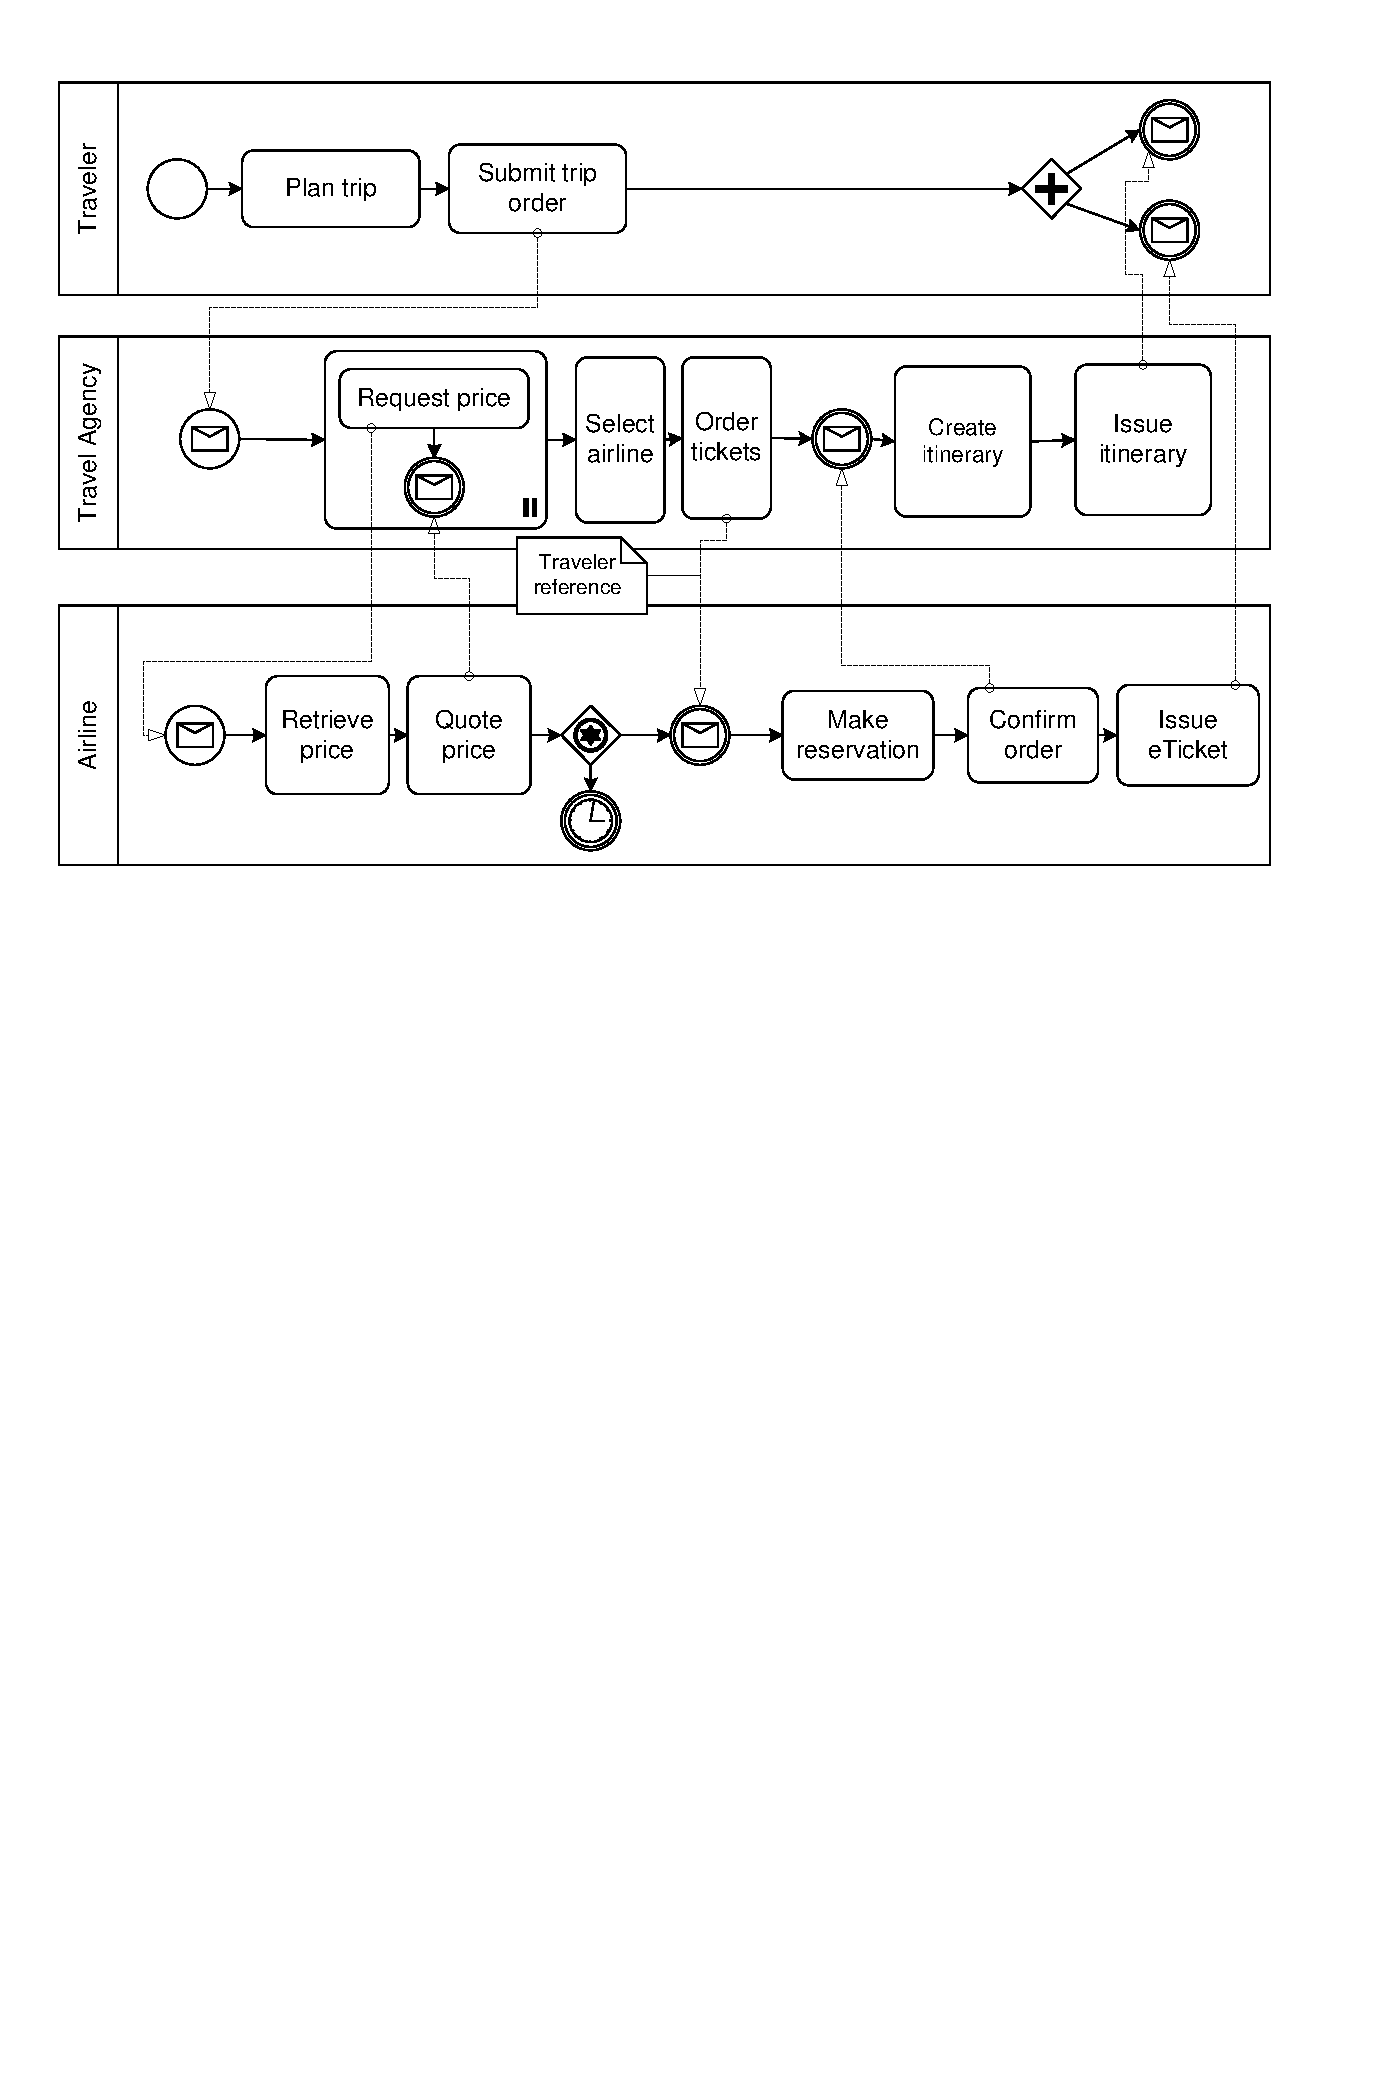
\includegraphics[width=0.9\paperheight]{choreography.pdf}
    \caption{Beispiel-Choreographie, auf einer weißen Seite gezeigt wird und über die definierten Seitenränder herausragt}
  \end{figure}
\end{landscape}

%the original layout is restored.
%%\restoregeometry cannot be used as we use \addtolength
\loadgeometry{koma}

\fi


\IfFileExists{pgfplots.sty}{
\section{Plots with pgfplots}
Pgfplot ist ein Paket um Graphen zu plotten ohne den Umweg über gnuplot oder matplotlib zu gehen.
\begin{figure}[h]
\begin{center}
\begin{tikzpicture}
  \begin{axis}[xlabel=$x$,
               ylabel=$\sin(x)$]
    \addplot {sin(deg(x))};  % Sinus-Funktion zeichnen
  \end{axis}
\end{tikzpicture}
\end{center}
\caption{$\sin(x)$ mit pgfplots.}
\end{figure}
}{}

\IfFileExists{tikz.sty}{
\section{Figures with tikz}
TikZ ist ein Paket um Zeichnungen mittels Programmierung zu erstellen.
Dieses Paket eignet sich um Gitter zu erstellen oder andere regelmäßige Strukturen zu erstellen.
\begin{figure}[ht]
\begin{center}
\begin{tikzpicture}
  \draw(0,0) rectangle (4,4);
  \foreach \x in {0.5,1,1.5,2,2.5,3,3.5}
    \foreach \y in {0.5,1,1.5,2,2.5,3,3.5}
      \draw(\x,\y) circle (1pt);
\end{tikzpicture}
\end{center}
\caption{Eine tikz-Graphik.}\label{fig:tikz_example}
\end{figure}
}{}

\section{Schlusswort}
Verbesserungsvorschläge für diese Vorlage sind immer willkommen.
Bitte bei GitHub ein Ticket eintragen (\url{https://github.com/latextemplates/uni-stuttgart-computer-science-template/issues}).

%% !TeX spellcheck = en_US
\allowdisplaybreaks
\chapter*{Listings}\label{chap:listing}
%TODO correct listings
\begin{Listing} 
	\caption{Generate Script Artifact Type}
	\label{lst:scripttype}
\begin{lstlisting}
public class RR_ScriptArtifactType {

@XmlRootElement(name = "tosca:Definitions")
@XmlAccessorType(XmlAccessType.PUBLIC_MEMBER)
public static class Definitions {

@XmlElement(name = "tosca:ArtifactType", required = true)
public ArtifactType artifactType;

@XmlAttribute(name = "xmlns:tosca", required = true)
public static final String tosca="http://docs.oasis-open.org/tosca/ns/2011/12";
@XmlAttribute(name = "xmlns:winery", required = true)
public static final String winery="http://www.opentosca.org/winery/extensions/tosca/2013/02/12";
@XmlAttribute(name = "xmlns:ns0", required = true)
public static final String ns0="http://www.eclipse.org/winery/model/selfservice";
@XmlAttribute(name = "id", required = true)
public static final String id="winery-defs-for_tbt-RR_ScriptArtifact";
@XmlAttribute(name = "targetNamespace", required = true)
public static final String targetNamespace="http://docs.oasis-open.org/tosca/ns/2011/12/ToscaBaseTypes"; 

public Definitions() {
artifactType = new ArtifactType();
}

public static class ArtifactType {
@XmlAttribute(name = "name", required = true)
public static final String name = "RR_ScriptArtifact";
@XmlAttribute(name = "targetNamespace", required = true)
public static final String targetNamespace="http://docs.oasis-open.org/tosca/ns/2011/12/ToscaBaseTypes"; 
ArtifactType() {}
}
}


}
\end{lstlisting}
\end{Listing}

\begin{Listing} 
	\caption{Generate definition for Script Artifact Type}
	\label{lst:scripttype_create}
	\begin{lstlisting}
// output filename
public static final String filename = "RR_ScriptArtifact.tosca";

/**
* Create ScriptType xml description
* 
* @param cr
* @throws JAXBException
* @throws IOException
*/
public static void init(Control_references cr) throws JAXBException,
IOException {
	File dir = new File(cr.getFolder() + Control_references.Definitions);
	dir.mkdirs();
	File temp = new File(cr.getFolder() + Control_references.Definitions + filename);
	if (temp.exists())
	temp.delete();
	temp.createNewFile();
	OutputStream output = new FileOutputStream(cr.getFolder()
	+ Control_references.Definitions + filename);
	
	JAXBContext jc = JAXBContext.newInstance(Definitions.class);
	
	Definitions shema = new Definitions();
	
	Marshaller marshaller = jc.createMarshaller();
	marshaller.setProperty(Marshaller.JAXB_FORMATTED_OUTPUT, true);
	marshaller.marshal(shema, output);
	cr.metaFile.addFileToMeta(Control_references.Definitions + filename, "application/vnd.oasis.tosca.definitions");
}
\end{lstlisting}
\end{Listing}
\begin{Listing}
\caption{Abstract language model}
\label{lst:langabst}
\begin{lstlisting}
public abstract class Language {
	
	// List of package managers supported by language
	protected List<PacketManager> packetManagers;
	
	// Extensions for this language
	protected List<String> extensions;
	
	// Language Name
	protected String Name;
	
	// To access package topology
	protected Control_references cr;
	
	// List with already created packages
	protected List <String> created_packages;
	
	/**
	* get Language name
	* 
	* @return
	*/
	public String getName() {
		return Name;
	}
	
	/**
	* Get supported extensions
	* 
	* @return list with extensions
	*/
	public List<String> getExtensions() {
		return extensions;
	}
	
	/**
	* Proceed file, transfer it to package managers
	* 
	* @param cr
	*            CSAR manager
	* @throws FileNotFoundException
	* @throws IOException
	* @throws JAXBException
	*/
	public void proceed(Control_references cr) throws FileNotFoundException,
	IOException, JAXBException {
		if (cr == null)
		throw new NullPointerException();
		for (String f : cr.getFiles())
		for (String suf : extensions)
		if (f.toLowerCase().endsWith(suf.toLowerCase()))
		for (PacketManager pm : packetManagers)
		pm.proceed(cr.getFolder() + f, f);
	}
	
	/**	Generate node name for specific packages
	* @param packet
	* @param source
	* @return
	*/
	public abstract String getNodeName(String packet, String source);
	
	
	/**	Generate Node for TOSCA Topology
	* @param packet
	* @param source
	* @return
	* @throws IOException
	* @throws JAXBException
	*/
	public abstract String createTOSCA_Node(String packet, String source) throws IOException, JAXBException;
}
\end{lstlisting}
\end{Listing}

\begin{Listing}
\caption{Abstract package manager model}
\label{lst:pmabst}
\begin{lstlisting}
public abstract class PacketManager {

// Name of manager
static public String Name;

protected Language language;

protected Control_references cr;

/**
* Proceed given file with different source (like archive)
* 
* @param filename
* @param cr
* @param source
* @throws FileNotFoundException
* @throws IOException
* @throws JAXBException
*/
public abstract void proceed(String filename, String source) throws FileNotFoundException, IOException,
JAXBException;
}
\end{lstlisting}
\end{Listing}

\begin{Listing}
\caption{Create TOSCA node for bash language}
\label{lst:create_bash}
\begin{lstlisting}
	public String createTOSCA_Node(String packet, String source) throws IOException, JAXBException{
if(created_packages.contains(packet+"+"+source))
return packet;
created_packages.add(packet+"+"+source);
packet = getNodeName(packet, source);
RR_NodeType.createNodeType(cr, packet);
RR_ScriptArtifactTemplate.createScriptArtifact(cr, packet);
RR_PackageArtifactTemplate.createPackageArtifact(cr, packet);
RR_TypeImplementation.createNT_Impl(cr, packet);
return packet;
}
\end{lstlisting}
\end{Listing}

%\begin{Listing}
%\begin{lstlisting}[caption={Create TOSCA node for bash language}\label{lst:create_bash},captionpos=t] 
%\end{lstlisting}
%\end{Listing}

\begin{Listing}
\caption{File parsing for Bash + apt-get }
\label{lst:bash_apt_parse}
\begin{lstlisting}
public void proceed(String filename, String source)
throws IOException, JAXBException {
String prefix = "";
for (int i = 0; i < Utils.getPathLength(filename) - 1; i++)
prefix = prefix + "../";
if (cr == null)
throw new NullPointerException();
System.out.println(Name + " proceed " + filename);
BufferedReader br = new BufferedReader(new FileReader(filename));
boolean isChanged = false;
String line = null;
String newFile = "";
while ((line = br.readLine()) != null) {
// split string to words
String[] words = line.replaceAll("[;&]", "").split("\\s+");
// skip space at the beginning of string
int i = 0;
if (words[i].equals(""))
i = 1;
// look for apt-get
if (words.length >= 1 + i && words[i].equals("apt-get")) {
// apt-get found
if (words.length >= 3 + i && words[1 + i].equals("install")) {
// replace "apt-get install" by "dpkg -i"
System.out.println("apt-get found:" + line);
isChanged = true;
for (int packet = 2 + i; packet < words.length; packet++) {
System.out.println("packet: " + words[packet]);
//							cr.AddDependenciesScript(source, words[packet]);
cr.getPacket(language, words[packet], source);
}
}
newFile += "#//References resolver//" + line + '\n';
} else
newFile += line + '\n';
}
br.close();
if (isChanged) {
// references found, need to replace file
// delete old
File file = new File(filename);
file.delete();

// create new file
FileWriter wScript = new FileWriter(file);
wScript.write(newFile, 0, newFile.length());
wScript.close();
}
}
\end{lstlisting}
\end{Listing}

\begin{Listing}
\caption{Ansible proceeding}
\label{lst:ansible_proceed}
\begin{lstlisting}
	public void proceed(Control_references cr) throws FileNotFoundException,
IOException, JAXBException {
	if (cr == null)
	throw new NullPointerException();
	for (String f : cr.getFiles())
	for (String suf : extensions)
	if (f.toLowerCase().endsWith(suf.toLowerCase())) {
		if (suf.equals(".zip")) {
			proceedZIP(f);
		} else
		proceed(f, f);
	}
}

/**
* proceed given file
* 
* @param filename
* @param cr
* @param source
*            of file, example - archive
* @throws FileNotFoundException
* @throws IOException
* @throws JAXBException
*/
public void proceed(String filename, String source)
throws FileNotFoundException, IOException, JAXBException {
	for (PacketManager pm : packetManagers)
	pm.proceed(filename, source);
}

/**
* Handle ZIP package
* 
* @param zipfile
* @throws FileNotFoundException
* @throws IOException
* @throws JAXBException
*/
private void proceedZIP(String zipfile) throws FileNotFoundException,
IOException, JAXBException {
	boolean isChanged = false;
	// String filename = new File(f).getName();
	String folder = new File(cr.getFolder() + zipfile).getParent()
	+ File.separator + "temp_RR_ansible_folder" + File.separator;
	List<String> files = zip.unZipIt(cr.getFolder() + zipfile, folder);
	for (String file : files)
	if (file.toLowerCase().endsWith("yml"))
	proceed(folder + file, zipfile);
	if (isChanged) {
		new File(cr.getFolder() + zipfile).delete();
		zip.zipIt(cr.getFolder() + zipfile, folder);
	}
	zip.delete(new File(folder));
	
}
\end{lstlisting}
\end{Listing}
%
%\renewcommand{\appendixtocname}{Anhang}
%\renewcommand{\appendixname}{Anhang}
%\renewcommand{\appendixpagename}{Anhang}
\appendix

\clearpage

%\printindex

\printbibliography

\ifdeutsch
Alle URLs wurden zuletzt am 17.\,03.\,2008 geprüft.
\else
All links were last followed on July 30, 2017.
\fi

\pagestyle{empty}
\renewcommand*{\chapterpagestyle}{empty}
\Versicherung
\end{document}
